%%%%%%%%%%%%%%%%%%%%%%%%%%%%%%%%%%%%%%%%%%%%%%%%%%%%%%%%%%%%%%%%%%%%%%%%%%%%%%%
%%  PLANTILLA PROYECTO DE GRADO
%%  Universidad de los Andes
%%  Departamento de Ingenieria de Sistemas y Computacion
%%
%%  Version LaTeX de "Plantilla_Proyecto_de_Grado.docx"
%%  Compilar con:  latexmk -xelatex main.tex     (recomendado)
%%             o:  latexmk -pdf main.tex         (pdfLaTeX)
%%%%%%%%%%%%%%%%%%%%%%%%%%%%%%%%%%%%%%%%%%%%%%%%%%%%%%%%%%%%%%%%%%%%%%%%%%%%%%%

\documentclass{plantilla-uniandes}

\usepackage{multirow}
\usepackage{tabularx}
\usepackage{booktabs}
\usepackage{array}

\newcolumntype{Y}{>{\raggedright\arraybackslash}X}
\newcolumntype{R}[1]{>{\raggedleft\arraybackslash}p{#1}}
\newcolumntype{L}[1]{>{\raggedright\arraybackslash}p{#1}}

% Diagramas
\usepackage{tikz}
\usetikzlibrary{arrows.meta,positioning,fit}

% Listados de codigo
\usepackage{listings}
\usepackage{xcolor}
\lstdefinelanguage{Rust}{
  morekeywords={as,break,const,continue,crate,else,enum,fn,for,if,impl,in,let,loop,match,mod,mut,pub,ref,return,self,Self,static,struct,trait,type,use,where,while,u8,u16,u32,u64,u128,usize,bool},
  sensitive=true,
  morecomment=[l]{//},
  morecomment=[s]{/*}{*/},
  morestring=[b]",
}
\lstset{
  basicstyle=\ttfamily\small,
  keywordstyle=\bfseries,
  commentstyle=\itshape\color{black!60},
  frame=single,
  columns=fullflexible,
  keepspaces=true,
  breaklines=true,
  aboveskip=1ex,
  belowskip=1ex,
}
\renewcommand{\lstlistingname}{Listado}

% Margen extra para que las palabras largas en monoespaciado no se salgan de la caja
\setlength{\emergencystretch}{1.5em}

%%-----------------------------------------------------------------------------
%% DATOS DEL TRABAJO  <-- edite unicamente estos valores
%%-----------------------------------------------------------------------------
\newcommand{\datoTitulo}{\textbf{\textbf{Evaluación de QPP-RNG como fuente de entropía para criptografía ligera en dispositivos IoT críticos} }}
\newcommand{\datoTituloLargo}{Evaluación de QPP-RNG como fuente de entropía para criptografía ligera en dispositivos IoT críticos}
\newcommand{\datoAutor}{Adrián Esteban Velásquez Solano \\ Juan Sebastián Sánchez}
\newcommand{\datoGrado}{Ingeniero de Sistemas y Computación}
\newcommand{\datoDirectorUno}{Ph.D. Carlos Andrés Lozano Garzón}
\newcommand{\datoGrupo}{COMIT}
\newcommand{\datoCiudad}{Bogotá D.C., Colombia}
\newcommand{\datoAnio}{2026}

% Titulo que aparece en el encabezado de las paginas pares
\settituloTesis{\datoTituloLargo}

\hypersetup{
  pdftitle={\datoTituloLargo},
  pdfauthor={\datoAutor},
  pdflang={es}
}

\begin{document}

\setlength{\parindent}{0pt}

\frontmatter   % numeracion en romanos MAYUSCULAS (I, II, III...)

%%=============================================================================
%% CUBIERTA
%% La cubierta y la portada no se numeran, pero si se cuentan como paginas.
%%=============================================================================
\begin{paginaPreliminar}
  \vspace*{2\baselineskip}
  \tituloPortada{\datoTitulo}

  \vspace{6\baselineskip}
  \textoPortada{\datoAutor}

  \vspace{6\baselineskip}
  Universidad de los Andes\\
  Departamento de Ingeniería de Sistemas y Computación\\
  Ingeniería de Sistemas y Computación\\
  \datoCiudad\\
  \datoAnio
\end{paginaPreliminar}

%%=============================================================================
%% PORTADA
%%=============================================================================
\begin{paginaPreliminar}
  \vspace*{2\baselineskip}
  \tituloPortada{\datoTituloLargo}

  \vspace{4\baselineskip}
  \textoPortada{\datoAutor}

  \vspace{3\baselineskip}
  Tesis presentada como requisito parcial para optar al título de:\\[0.5\baselineskip]
  \textbf{\datoGrado}

  \vspace{3\baselineskip}
  Director:\\
  \datoDirectorUno\\
 

  \vspace{3\baselineskip}
  Grupo de Investigación:\\
  \datoGrupo

  \vspace{3\baselineskip}
  Universidad de los Andes\\
  Departamento de Ingeniería de Sistemas y Computación\\
  Ingeniería de Sistemas y Computación\\
  \datoCiudad\\
  \datoAnio
\end{paginaPreliminar}

%%=============================================================================
%% DEDICATORIA O LEMA  (opcional)
%%=============================================================================
\cleardoublepage
\thispagestyle{empty}
{\raggedleft
  \emph{(Dedicatoria o lema)}\par
  \vspace{6\baselineskip}
  \begin{minipage}{0.62\textwidth}
    \itshape\justifying
    Su uso es opcional y cada autor podrá determinar la distribución del texto
    en la página, se sugiere esta presentación. En ella el autor del trabajo
    dedica su trabajo en forma especial a personas y/o entidades.

    Por ejemplo:

    A mis padres

    o

    La preocupación por el hombre y su destino siempre debe ser el interés
    primordial de todo esfuerzo técnico. Nunca olvides esto entre tus diagramas
    y ecuaciones.

    Albert Einstein
  \end{minipage}\par
}
\clearpage

%%=============================================================================
%% AGRADECIMIENTOS  (opcional)
%%=============================================================================
\cleardoublepage
\tituloPreliminarSinTDC{Agradecimientos}

Esta sección es opcional, en ella el autor agradece a las personas o
instituciones que colaboraron en la realización del trabajo. Si se incluye esta
sección, deben aparecer los nombres completos, los cargos y su aporte al
trabajo.

A continuación, se presenta la tabla de contenido la cual se actualiza
automáticamente. En \LaTeX{} basta con volver a compilar el documento (dos
veces) para que la tabla de contenido, la lista de figuras, la lista de tablas
y las referencias cruzadas queden actualizadas.

Esta plantilla reproduce las secciones del documento original: cubierta,
portada, dedicatoria, agradecimientos, resumen, contenido, listas, cuerpo,
anexos y bibliografía. Es importante conservar dicha estructura.

%%=============================================================================
%% RESUMEN
%%=============================================================================
\cleardoublepage
% "Pag." debe quedar como primera linea del archivo .toc, es decir, antes de
% que Resumen escriba su propia entrada.
\addtocontents{toc}{\protect\encabezadoPag}
\tituloResumen{Resumen}

Los dispositivos IoT críticos necesitan claves impredecibles, pero muchos microcontroladores carecen de un generador físico de números aleatorios. QPP-RNG, una propuesta reciente que obtiene entropía del \textit{jitter} de ejecución de una caminata de permutaciones, ha sido evaluado favorablemente con las pruebas del NIST en computadores de propósito general. Este trabajo diseñó, implementó en Rust y evaluó una librería que integra QPP-RNG con Ascon-AEAD128 (NIST SP 800-232), con pruebas sobre un Arduino Mega 2560, un Arduino Nano y un nRF52840. En los tres microcontroladores, la salida de la referencia fue idéntica bit a bit tras cada reinicio y, aun así, superó las pruebas estadísticas. En una Raspberry Pi 4 y un computador con Windows, cada ciclo aportó solo entre 0.375 y 0.407 bits de min-entropía según NIST SP 800-90B, unos 2 bits por byte frente a los 8 contabilizados, un déficit que ninguna prueba de la salida detectó. La variante propuesta toma su entropía de un oscilador físicamente independiente (el perro guardián en AVR, con al menos 1.62 bits por muestra, y el RNG del nRF52840), aplica pruebas de salud continuas y contabiliza la entropía de forma explícita. Su salida difiere tras cada reinicio, supera las pruebas evaluadas y alcanza 7.4 B/s en AVR y 101 B/s en el nRF52840, y la pila completa cabe en 16 KB de Flash. Se concluye que QPP-RNG en su forma original no es viable en microcontroladores sin sistema operativo, y que toda afirmación de entropía debe basarse en evaluar la fuente, no la salida.

\textbf{Palabras clave:} generación de números aleatorios, min-entropía, QPP-RNG, criptografía ligera, Ascon, Internet de las cosas, Rust.

%%=============================================================================
%% ABSTRACT
%%=============================================================================
\cleardoublepage
\tituloResumen{Abstract}

Critical IoT devices need unpredictable keys and nonces, yet many microcontrollers have no physical random number generator. QPP-RNG, a recent proposal that draws entropy from the execution jitter of a permutation walk, has been assessed favourably with NIST tests on general-purpose platforms. This work designed, implemented in Rust and evaluated a library that integrates QPP-RNG with Ascon-AEAD128 (NIST SP 800-232): a faithful implementation of the generator, a microcontroller variant, a SHA-256 conditioner, an evaluation harness and test firmware for an Arduino Mega 2560, an Arduino Nano and an nRF52840. On all three microcontrollers, the reference generator's output was bit-for-bit identical after every reset, and it still passed the statistical tests. On a Raspberry Pi 4 and a Windows desktop, each cycle contributed only 0.375 to 0.407 bits of min-entropy according to NIST SP 800-90B, about 2 bits per byte against the 8 accounted for, a shortfall that no output-level test detected. The proposed variant draws its entropy from a physically independent oscillator (the AVR watchdog, at 1.62 to 2.24 bits per sample, and the nRF52840 hardware RNG, at 7.24 bits per byte), applies continuous health tests and accounts for entropy explicitly. Its output differs after every reset, passes the tests applied and reaches 7.4 B/s on AVR and 101 B/s on the nRF52840; the full stack takes 16 KB of flash on AVR. The original QPP-RNG is therefore not viable on bare-metal microcontrollers, and any entropy claim must rest on an assessment of the source, not of the output.

\textbf{Keywords:} random number generation, min-entropy, QPP-RNG, lightweight cryptography, Ascon, Internet of Things, Rust.

%%=============================================================================
%% CONTENIDO
%%=============================================================================
\cleardoublepage
\tableofcontents

%%=============================================================================
%% LISTA DE FIGURAS
%%=============================================================================
\cleardoublepage
\phantomsection
\markboth{\listfigurename}{\listfigurename}
\addcontentsline{toc}{chapter}{\listfigurename}
\addtocontents{lof}{\protect\encabezadoPag}
\listoffigures

%%=============================================================================
%% LISTA DE TABLAS
%%=============================================================================
\cleardoublepage
\phantomsection
\markboth{\listtablename}{\listtablename}
\addcontentsline{toc}{chapter}{\listtablename}
\addtocontents{lot}{\protect\encabezadoPag}
\listoftables

%%=============================================================================
%% LISTA DE SIMBOLOS Y ABREVIATURAS  (opcional)
%%=============================================================================
%%=============================================================================
%% LISTA DE SIMBOLOS Y ABREVIATURAS
%% Los subtitulos de cada tipo de simbolo van en Arial 14 pt y en negrilla.
%% Las tablas de esta seccion no llevan bordes (igual que en el original).
%%=============================================================================
\cleardoublepage
\tituloPreliminar{Lista de Símbolos y abreviaturas}

\needspace{8\baselineskip}
{\bfseries\fontsize{14}{16}\selectfont Símbolos con letras latinas\par}
\nopagebreak\vspace{0.5ex}
{\small\interlineadoSencillo\setlength{\LTleft}{0pt}\setlength{\LTright}{0pt plus 1fill}
\begin{longtable}{@{}p{1.7cm}p{7.3cm}p{1.9cm}p{3.1cm}@{}}
\textbf{Símbolo} & \textbf{Término} & \textbf{Unidad} & \textbf{Definición}\\[0.6ex]
\endhead
$C_{\text{APT}}$ & Umbral de la prueba de proporción adaptativa & muestras & Sección~\ref{sec:variante_iot}\\[0.6ex]
$C_{\text{RCT}}$ & Umbral de la prueba de conteo de repeticiones & muestras & Sección~\ref{sec:variante_iot}\\[0.6ex]
$H$ & Min-entropía acreditada a una muestra & bits & Sección~\ref{sec:variante_iot}\\[0.6ex]
$H(X)$ & Entropía de Shannon & bits & Sección~\ref{sec:aleatoriedad_entropia}\\[0.6ex]
$H_{\infty}(X)$ & Min-entropía & bits & Sección~\ref{sec:aleatoriedad_entropia}\\[0.6ex]
$k$ & Resolución del temporizador & ticks & Ec.~\eqref{eq:normalizacion}\\[0.6ex]
$m$ & Ciclos por byte (sobremuestreo) & 1 & Sección~\ref{sec:referencia}\\[0.6ex]
$N$ & Número de elementos de la permutación & 1 & Sección~\ref{sec:referencia}\\[0.6ex]
$n_p$ & \textit{Pads} generados hasta volver a la identidad & 1 & Sección~\ref{sec:referencia}\\[0.6ex]
$p_7$ & Probabilidad de que el bit 7 valga 1 & 1 & Ec.~\eqref{eq:sesgo_bit7}\\[0.6ex]
$S_N$ & Grupo simétrico de grado $N$ & -- & Sección~\ref{sec:referencia}\\[0.6ex]
$s$ & Semilla del generador & bits & Sección~\ref{sec:referencia}\\[0.6ex]
$W$ & Ventana de la prueba de proporción adaptativa & muestras & Sección~\ref{sec:variante_iot}\\
\end{longtable}}

\needspace{8\baselineskip}
{\bfseries\fontsize{14}{16}\selectfont Símbolos con letras griegas\par}
\nopagebreak\vspace{0.5ex}
{\small\interlineadoSencillo\setlength{\LTleft}{0pt}\setlength{\LTright}{0pt plus 1fill}
\begin{longtable}{@{}p{1.7cm}p{7.3cm}p{1.9cm}p{3.1cm}@{}}
\textbf{Símbolo} & \textbf{Término} & \textbf{Unidad} & \textbf{Definición}\\[0.6ex]
\endhead
$\alpha$ & Nivel de significancia o tasa de falsos positivos & 1 & Sección~\ref{sec:evaluacion_estadistica}\\[0.6ex]
$\delta$ & Tiempo normalizado de un ciclo & 1 & Ec.~\eqref{eq:normalizacion}\\[0.6ex]
$\Delta t$ & Duración de un ciclo de convergencia & ticks & Sección~\ref{sec:referencia}\\[0.6ex]
$\sigma$ & Desviación estándar & ciclos & Sección~\ref{sec:res_fuentes}\\
\end{longtable}}

\clearpage
{\bfseries\fontsize{14}{16}\selectfont Abreviaturas\par}
\nopagebreak\vspace{0.5ex}
{\small\interlineadoSencillo\setlength{\LTleft}{0pt}\setlength{\LTright}{0pt plus 1fill}
\begin{longtable}{@{}p{3.0cm}p{11.0cm}@{}}
\textbf{Abreviatura} & \textbf{Término}\\[0.6ex]
\endhead
ACVP & \textit{Automated Cryptographic Validation Protocol}\\[0.6ex]
ADC & \textit{Analog-to-Digital Converter}, convertidor analógico-digital\\[0.6ex]
AEAD & \textit{Authenticated Encryption with Associated Data}\\[0.6ex]
AES & \textit{Advanced Encryption Standard}\\[0.6ex]
APT & \textit{Adaptive Proportion Test}, prueba de proporción adaptativa\\[0.6ex]
ARX & \textit{Addition, Rotation, XOR}\\[0.6ex]
AVR & Microcontroladores de 8 bits de Microchip (antes Atmel)\\[0.6ex]
CAVP & \textit{Cryptographic Algorithm Validation Program}\\[0.6ex]
CSPRNG & \textit{Cryptographically Secure Pseudo Random Number Generator}\\[0.6ex]
DRBG & \textit{Deterministic Random Bit Generator}\\[0.6ex]
ENT & Programa de análisis estadístico de secuencias de bytes\\[0.6ex]
HIL & \textit{Hardware-in-the-loop}, pruebas sobre hardware\\[0.6ex]
IID & Independiente e idénticamente distribuido\\[0.6ex]
IoT & \textit{Internet of Things}, Internet de las cosas\\[0.6ex]
KAT & \textit{Known Answer Test}, prueba de respuesta conocida\\[0.6ex]
LFRC & \textit{Low-Frequency RC oscillator}\\[0.6ex]
LRS & \textit{Longest Repeated Substring}, estimador de SP 800-90B\\[0.6ex]
LTO & \textit{Link-Time Optimization}\\[0.6ex]
LWC & \textit{Lightweight Cryptography}, criptografía ligera\\[0.6ex]
MCV & \textit{Most Common Value}, estimador de SP 800-90B\\[0.6ex]
NIST & \textit{National Institute of Standards and Technology}\\[0.6ex]
OTP & \textit{One-Time Pad}\\[0.6ex]
PRNG & \textit{Pseudo Random Number Generator}\\[0.6ex]
QPP & \textit{Quantum Permutation Pad}\\[0.6ex]
QPP-RNG & \textit{Quantum Permutation Pad Random Number Generator}\\[0.6ex]
RCT & \textit{Repetition Count Test}, prueba de conteo de repeticiones\\[0.6ex]
RNG & \textit{Random Number Generator}\\[0.6ex]
RTC & \textit{Real-Time Counter} (nRF52840) o \textit{Real-Time Clock} (ESP32)\\[0.6ex]
SAR & \textit{Successive Approximation Register}, ADC de aproximaciones sucesivas\\[0.6ex]
SHA & \textit{Secure Hash Algorithm}\\[0.6ex]
SP & \textit{Special Publication} del NIST\\[0.6ex]
SPN & \textit{Substitution-Permutation Network}\\[0.6ex]
STS & \textit{Statistical Test Suite} del NIST (SP 800-22)\\[0.6ex]
TRNG & \textit{True Random Number Generator}\\[0.6ex]
UART & \textit{Universal Asynchronous Receiver-Transmitter}\\[0.6ex]
WSL & \textit{Windows Subsystem for Linux}\\
\end{longtable}}

\mainmatter   % numeracion arabiga reiniciando en 1

%%=============================================================================
%% INTRODUCCION
%%=============================================================================
%%=============================================================================
%% INTRODUCCION
%% Titulo sin numerar, Arial 20 pt negrilla, 100 pt antes / 24 pt despues.
%%=============================================================================
\tituloPreliminar{Introducción}

Durante la última década, el Internet de las Cosas (Internet of Things, IoT) ha experimentado un crecimiento acelerado, transformando la forma en que los sistemas físicos interactúan con infraestructuras digitales mediante sensores, actuadores y dispositivos embebidos interconectados. Actualmente, el IoT constituye uno de los principales pilares de la denominada Industria 4.0 y soporta aplicaciones críticas en sectores como la salud, el transporte inteligente, la manufactura avanzada, la agricultura de precisión, las ciudades inteligentes y la infraestructura energética. La incorporación masiva de dispositivos conectados ha permitido incrementar los niveles de automatización, monitoreo en tiempo real y toma de decisiones basada en datos, favoreciendo procesos más eficientes y una mayor capacidad de respuesta frente a eventos dinámicos. Sin embargo, esta misma expansión ha incrementado significativamente la superficie de ataque disponible para actores maliciosos, convirtiendo la seguridad informática en uno de los principales desafíos tecnológicos de la actualidad.

Las proyecciones internacionales estiman que durante los próximos años existirán decenas de miles de millones de dispositivos IoT desplegados alrededor del mundo, muchos de ellos desempeñando funciones críticas relacionadas con infraestructura esencial, servicios médicos, redes eléctricas, transporte público e instalaciones industriales \cite{Sinha2025StateGlobally}. A diferencia de los sistemas informáticos tradicionales, estos dispositivos suelen operar durante largos periodos de tiempo sin supervisión directa, poseen capacidades limitadas de procesamiento, memoria y almacenamiento, y frecuentemente dependen de baterías o mecanismos de alimentación con restricciones energéticas severas. Estas características hacen que la implementación de mecanismos criptográficos convencionales resulte costosa o incluso inviable desde el punto de vista computacional, generando la necesidad de desarrollar soluciones específicamente diseñadas para ambientes con recursos restringidos \cite{McKay2017ReportCryptography,Thakor2021LightweightOpportunities}. Diversos estudios recientes coinciden en que la seguridad de los sistemas IoT debe abordarse mediante algoritmos capaces de ofrecer altos niveles de protección utilizando una cantidad mínima de memoria, ciclos de procesamiento y consumo energético \cite{Dhanda2020LightweightIoT,Seyhan2022ClassificationTaxonomy}.

Como respuesta a estas limitaciones surgió el área de investigación conocida como \textit{Lightweight Cryptography} (LWC), cuyo propósito consiste en diseñar mecanismos criptográficos capaces de preservar las propiedades fundamentales de confidencialidad, integridad, autenticidad y disponibilidad utilizando recursos considerablemente inferiores a los requeridos por algoritmos tradicionales \cite{McKay2017ReportCryptography}. La criptografía ligera no busca reemplazar completamente los estándares clásicos, sino proporcionar alternativas especialmente adaptadas a plataformas embebidas donde cada kilobyte de memoria, cada ciclo de reloj y cada miliwatt de energía representan recursos escasos. Durante la última década, esta área ha recibido un interés creciente tanto por parte de la comunidad científica como de organismos internacionales de estandarización, impulsando el desarrollo de nuevos algoritmos optimizados para microcontroladores, sensores inalámbricos y sistemas ciberfísicos \cite{Althobaiti2025LightweightStandardization,Radhakrishnan2024EfficiencyDevices}.

La importancia de esta línea de investigación llevó al National Institute of Standards and Technology (NIST) a iniciar en 2018 el proceso internacional de estandarización de algoritmos de criptografía ligera \cite{McKay2017ReportCryptography}. Después de evaluar decenas de propuestas provenientes de universidades, centros de investigación e industria, el proceso concluyó con la selección de ASCON como nuevo estándar para autenticación y cifrado autenticado en dispositivos con restricciones computacionales \cite{NationalInstituteofStandards2023AnnouncingSelection,Turan2025Ascon-BasedFunctions}. La elección de ASCON respondió a su capacidad para ofrecer elevados niveles de seguridad junto con un excelente desempeño tanto en implementaciones software como hardware, convirtiéndose actualmente en el principal referente para el desarrollo de aplicaciones IoT seguras \cite{Dobraunig2021AsconHashing}. No obstante, aun cuando ASCON proporciona mecanismos robustos para proteger la información transmitida, la seguridad global del sistema continúa dependiendo de la calidad del material criptográfico utilizado durante la generación de claves, semillas, vectores de inicialización y números aleatorios \cite{Katz2020IntroductionCryptography}.

La generación de números aleatorios constituye uno de los componentes más críticos dentro de cualquier arquitectura criptográfica moderna. Diversos ataques históricos han demostrado que incluso algoritmos considerados matemáticamente seguros pueden verse completamente comprometidos cuando utilizan fuentes de entropía deficientes o generadores de números pseudoaleatorios con baja calidad estadística \cite{Katz2020IntroductionCryptography,Menezes1996HandbookCryptography}. En consecuencia, la fortaleza de protocolos criptográficos, sistemas de autenticación, firmas digitales y mecanismos de establecimiento de claves depende directamente de la capacidad del sistema para producir secuencias impredecibles, no reproducibles y estadísticamente uniformes. Por esta razón, organismos como el NIST han desarrollado estándares específicos para la evaluación de fuentes de entropía, incluyendo las recomendaciones SP 800-22 para pruebas estadísticas, SP 800-90A para generadores determinísticos y SP 800-90B para estimación de entropía en fuentes físicas y no determinísticas \cite{Rukhin2010AApplications,Barker2015RecommendationGenerators,Turan2018RecommendationGeneration}.

Tradicionalmente, la obtención de entropía en dispositivos IoT ha dependido de generadores de números aleatorios implementados mediante hardware (\textit{True Random Number Generators}, TRNG), los cuales aprovechan fenómenos físicos como ruido térmico, osciladores de anillo, variaciones eléctricas o procesos cuánticos para producir secuencias impredecibles \cite{Seyhan2022ClassificationTaxonomy}. Aunque estos mecanismos ofrecen elevados niveles de seguridad, presentan limitaciones importantes relacionadas con el costo de implementación, la disponibilidad del hardware, la portabilidad entre plataformas y la complejidad de validación. En muchos dispositivos de bajo costo, especialmente aquellos destinados a aplicaciones masivas del Internet de las Cosas, la incorporación de hardware especializado resulta económicamente inviable, motivando la búsqueda de alternativas software capaces de generar niveles adecuados de entropía utilizando únicamente los recursos disponibles en el sistema operativo y la microarquitectura del procesador.

En este contexto surge \textit{Quantum Permutation Pad Random Number Generator} (QPP-RNG), una propuesta reciente desarrollada por Quantropi Inc. basada en la obtención de entropía mediante múltiples fuentes de comportamiento interno del sistema computacional \cite{Kuang2025QPP-RNG:Randomness,Kuang2025IID-BasedJitter}. A diferencia de los enfoques tradicionales, QPP-RNG combina información proveniente del \textit{system jitter}, tiempos de ejecución, acceso a memoria, variaciones microarquitecturales, comportamiento del planificador del sistema operativo y otros eventos no determinísticos para construir una fuente de entropía completamente implementada en software. Los resultados publicados muestran que este mecanismo alcanza niveles de min-entropía cercanos al máximo teórico permitido por byte y supera satisfactoriamente las principales pruebas estadísticas internacionalmente aceptadas, incluyendo NIST SP 800-22, NIST SP 800-90B y ENT, posicionándose como una alternativa prometedora para aplicaciones criptográficas de alta seguridad sin requerir hardware adicional \cite{Vrana2025RawEvaluation,Walker2008ENT:Program}.

Paralelamente, el avance acelerado de la computación cuántica ha introducido nuevos desafíos para la seguridad de los sistemas criptográficos actuales. Algoritmos como el propuesto por Shor demuestran que los principales esquemas de criptografía asimétrica utilizados actualmente, entre ellos RSA y la criptografía de curva elíptica (ECC), podrán ser vulnerables una vez existan computadores cuánticos suficientemente grandes y tolerantes a fallos \cite{Shor1994AlgorithmsFactoring,Ivezic2017ShorsCryptography}. Aunque la criptografía ligera se concentra principalmente en algoritmos simétricos, la transición hacia ecosistemas resistentes a la computación cuántica requiere fortalecer todos los componentes de la arquitectura criptográfica, incluyendo la generación de material aleatorio de alta calidad. Dentro de este escenario, Quantum Permutation Pad (QPP) ha sido propuesto como un marco criptográfico capaz de aprovechar propiedades derivadas de espacios de permutaciones para construir mecanismos resistentes frente a ataques clásicos y cuánticos, ofreciendo además niveles significativamente superiores de entropía respecto a enfoques tradicionales \cite{Kuang2022QuantumCryptography,Kuang2020ShannonSpace}.

A pesar de los resultados obtenidos por QPP y QPP-RNG, actualmente existe una brecha importante entre las propuestas teóricas disponibles en la literatura y su utilización práctica dentro de dispositivos IoT críticos. En particular, no se dispone de implementaciones abiertas, modulares y optimizadas que permitan integrar QPP-RNG como fuente de entropía dentro de arquitecturas modernas de criptografía ligera. Asimismo, existe una limitada evidencia experimental respecto al comportamiento de este mecanismo sobre plataformas embebidas, especialmente en términos de consumo de memoria, utilización del procesador, rendimiento, calidad estadística y facilidad de integración con algoritmos ligeros ampliamente utilizados como ASCON.

En este contexto, la presente investigación propone el diseño, implementación y evaluación de una librería criptográfica ligera desarrollada en el lenguaje de programación Rust, incorporando una adaptación optimizada de QPP-RNG como fuente de entropía para dispositivos IoT críticos. Rust fue seleccionado debido a sus mecanismos de seguridad de memoria, ausencia de \textit{data races}, modelo de propiedad (\textit{ownership}) y creciente adopción dentro del desarrollo de software seguro para infraestructura crítica. La investigación contempla el análisis integral de la calidad estadística de los números aleatorios generados, el estudio del consumo de recursos computacionales, la evaluación del desempeño frente a soluciones de referencia y la validación de la viabilidad práctica de incorporar QPP-RNG dentro de arquitecturas de criptografía ligera orientadas a sistemas embebidos.

Finalmente, esta investigación busca contribuir simultáneamente en tres dimensiones. Desde la perspectiva científica, amplía el conocimiento existente sobre la utilización de nuevas fuentes de entropía software para criptografía ligera y seguridad post-cuántica. Desde el punto de vista tecnológico, desarrolla una librería modular reutilizable que podrá servir como base para futuras investigaciones y aplicaciones industriales. Finalmente, desde una perspectiva práctica, proporciona evidencia experimental acerca de la viabilidad de incorporar mecanismos avanzados de generación de entropía dentro de dispositivos IoT con restricciones severas de memoria, procesamiento y consumo energético, contribuyendo al fortalecimiento de la seguridad de la próxima generación de sistemas inteligentes conectados.

%%=============================================================================
%% CAPITULOS
%%=============================================================================

%%=============================================================================
%% ESTADO DEL ARTE
%%=============================================================================
\chapter{Estado del arte}

La seguridad de los sistemas embebidos y del Internet de las Cosas constituye actualmente una de las principales áreas de investigación dentro de la ciberseguridad moderna. El crecimiento exponencial del número de dispositivos conectados \cite{Sinha2025StateGlobally}, junto con el avance de la computación distribuida, el \textit{edge computing} y las ciudades inteligentes, ha incrementado significativamente la necesidad de desarrollar mecanismos criptográficos capaces de operar bajo severas restricciones de memoria, capacidad de procesamiento y consumo energético.

Durante los últimos años, la comunidad científica ha concentrado sus esfuerzos en tres líneas principales de investigación. La primera corresponde al diseño de algoritmos de criptografía ligera que permitan proteger la información utilizando una cantidad reducida de recursos computacionales. La segunda se enfoca en el desarrollo de mecanismos resistentes frente a la futura amenaza de la computación cuántica. Finalmente, una tercera línea de investigación, menos explorada pero igualmente crítica, estudia la generación de números aleatorios de alta calidad como fundamento de cualquier sistema criptográfico seguro.

El presente capítulo revisa el estado del conocimiento en estas tres áreas, iniciando con una descripción de la evolución del Internet de las Cosas y sus restricciones computacionales, continuando con los principales desafíos de seguridad presentes en estos entornos. Posteriormente, se analiza la evolución de la criptografía ligera y de los mecanismos modernos de generación de entropía, para finalmente estudiar los fundamentos del \textit{Quantum Permutation Pad} (QPP) y \textit{Quantum Permutation Pad Random Number Generator} (QPP-RNG), identificando las brechas existentes en la literatura que motivan la presente investigación.


%%=========== 
%% SECCION 1
%%=========== 

\section{Internet de las cosas: evolución, arquitectura y restricciones}

El concepto de Internet de las Cosas (\textit{Internet of Things}, IoT) hace referencia a la interconexión de objetos físicos capaces de percibir información del entorno mediante sensores, procesarla localmente y transmitirla a través de diferentes tecnologías de comunicación hacia otros dispositivos o plataformas de procesamiento. Aunque el término fue propuesto por Kevin Ashton a finales de la década de los noventa \cite{Dhanda2020LightweightIoT}, solamente durante la última década, la disponibilidad de sensores de bajo costo, redes inalámbricas, servicios en la nube y plataformas de análisis masivo de datos permitieron su adopción a gran escala.

Actualmente el IoT constituye uno de los principales habilitadores tecnológicos de la Industria 4.0. Este permite integrar procesos físicos y digitales mediante arquitecturas distribuidas donde  millones de dispositivos trabajan de la mano para monitorear y controlar procesos en tiempo real. Esta evolución ha favorecido el desarrollo de aplicaciones en múltiples dominios, incluyendo ciudades inteligentes, automatización industrial, agricultura de precisión y sistemas de transporte inteligente, entre otros.
Desde una perspectiva arquitectónica, la mayoría de implementaciones IoT pueden describirse mediante un modelo jerárquico compuesto por cuatro niveles principales.

El primer nivel corresponde a la capa de percepción, integrada por sensores, actuadores y dispositivos embebidos encargados de capturar información del entorno físico. Estos dispositivos representan el punto de conexión entre el mundo físico y el mundo digital. Generalmente poseen capacidades computacionales extremadamente limitadas.

El segundo nivel corresponde a la capa de comunicación, responsable del transporte seguro de la información utilizando tecnologías como Wi-Fi, Bluetooth Low Energy (BLE), Zigbee, Thread, LoRaWAN, NB-IoT, Ethernet industrial y redes celulares de quinta generación (5G). Cada tecnología presenta ventajas particulares en términos de alcance, ancho de banda, latencia y consumo energético, condicionando directamente las soluciones criptográficas que pueden implementarse.

En tercer lugar, la capa de procesamiento incorpora nodos Edge, Fog o servicios Cloud donde se ejecutan procesos de almacenamiento, agregación de datos, análisis estadístico, inteligencia artificial y automatización.

Finalmente, la capa de aplicación implementa la lógica de negocio específica para cada dominio, proporcionando servicios a usuarios finales, operadores industriales o sistemas de apoyo a la toma de decisiones.

Uno de los aspectos que diferencia al Internet de las Cosas de los sistemas informáticos tradicionales radica en las severas restricciones de recursos presentes en la mayoría de dispositivos embebidos. Mientras un computador personal moderno dispone de varios gigabytes de memoria RAM, múltiples núcleos de procesamiento y almacenamiento de estado sólido, gran parte de los microcontroladores utilizados en aplicaciones IoT operan con frecuencias inferiores a los 100 MHz, memorias RAM del orden de pocos kilobytes y capacidades de almacenamiento inferiores a un megabyte.

Estas limitaciones afectan directamente la implementación de mecanismos criptográficos convencionales. Algoritmos ampliamente utilizados como RSA, ECC o incluso implementaciones completas de AES pueden consumir una fracción considerable de la memoria disponible o incrementar significativamente el tiempo de procesamiento requerido para cada operación criptográfica. De igual manera, muchos dispositivos funcionan mediante baterías cuya autonomía debe extenderse durante varios años, haciendo indispensable minimizar el número de operaciones matemáticas ejecutadas y reducir al máximo el consumo energético asociado a los procesos de autenticación y cifrado. Estudios recientes muestran que incluso pequeños incrementos en la complejidad computacional pueden traducirse en reducciones significativas de la vida útil de los dispositivos desplegados en campo \cite{Radhakrishnan2024EfficiencyDevices}.

Las restricciones descritas anteriormente han motivado la aparición del concepto de dispositivos con recursos restringidos (\textit{resource-constrained devices}). Diversos organismos internacionales, incluyendo el Internet Engineering Task Force (IETF) y el National Institute of Standards and Technology (NIST), clasifican estos dispositivos según su capacidad de memoria, procesamiento y energía disponible \cite{McKay2017ReportCryptography}. En particular, los dispositivos pertenecientes a las clases más bajas pueden disponer únicamente de algunos kilobytes de memoria RAM y capacidades de procesamiento limitadas, haciendo prácticamente imposible la ejecución de protocolos criptográficos diseñados originalmente para computadores.

Como consecuencia, el diseño de soluciones de seguridad para IoT requiere optimizar simultáneamente múltiples variables: tiempo de ejecución, utilización de memoria, consumo energético, tamaño del código ejecutable, ancho de banda requerido para transmisión y resistencia frente a ataques criptográficos. Esta combinación de restricciones convierte al Internet de las Cosas en uno de los escenarios más exigentes para el diseño de algoritmos criptográficos modernos.

Otro aspecto diferenciador del IoT consiste en la heterogeneidad de sus componentes y características físicas. En una misma arquitectura pueden coexistir microcontroladores ARM Cortex-M, procesadores RISC-V, ESP32, AVR, FPGA e incluso computadores industriales de altas capacidades. Esta diversidad dificulta el desarrollo de bibliotecas criptográficas portables y obliga a diseñar implementaciones suficientemente flexibles para adaptarse a múltiples arquitecturas sin comprometer la seguridad ni el rendimiento.

Adicionalmente, la naturaleza distribuida de estos sistemas incrementa la complejidad de la gestión de claves criptográficas, la autenticación mutua entre dispositivos y la actualización segura del software. Miles de dispositivos pueden permanecer desplegados durante años en ubicaciones remotas donde las tareas de mantenimiento físico resultan costosas o incluso inviables. Bajo estas condiciones, cualquier vulnerabilidad criptográfica puede permanecer explotable durante largos periodos de tiempo, afectando simultáneamente un gran número de nodos dentro de la infraestructura.

En consecuencia, la comunidad científica coincide en que la seguridad del Internet de las Cosas no puede abordarse simplemente trasladando las soluciones desarrolladas para sistemas tradicionales. Las restricciones computacionales, la heterogeneidad del hardware, la escalabilidad de las implementaciones y la necesidad de minimizar el consumo energético requieren mecanismos específicamente diseñados para estos escenarios. Esta necesidad dio origen a una nueva línea de investigación conocida como Criptografía Ligera (Lightweight Cryptography), cuyo objetivo consiste en proporcionar niveles elevados de seguridad manteniendo simultáneamente un consumo reducido de recursos computacionales \cite{McKay2017ReportCryptography,NationalInstituteofStandards2023AnnouncingSelection}. Dicho paradigma constituye actualmente una de las principales áreas de investigación dentro de la seguridad informática aplicada a sistemas embebidos e infraestructura crítica.


%%=========== 
%% SECCION 2
%%=========== 

\section{Seguridad en dispositivos IoT}

La seguridad constituye uno de los principales retos para la adopción masiva del Internet de las Cosas. A diferencia de los sistemas informáticos convencionales, los dispositivos IoT operan en entornos altamente distribuidos, heterogéneos y en muchos casos, físicamente accesibles para atacantes potenciales. Esta combinación de restricciones computacionales, conectividad permanente y despliegues de gran escala ha incrementado significativamente la superficie de ataque de las infraestructuras digitales modernas, convirtiendo la protección de estos sistemas en una prioridad tanto para la comunidad científica como para organismos gubernamentales y el sector industrial.

La mayoría de los dispositivos IoT son diseñados para desempeñar funciones específicas durante largos periodos de tiempo con una mínima intervención humana. En consecuencia, suelen permanecer conectados de manera continua a redes públicas o privadas, transmitiendo información sensible relacionada con procesos industriales, variables ambientales, datos médicos o infraestructura crítica. Cualquier vulnerabilidad presente en estos dispositivos puede comprometer no solamente la confidencialidad de la información, sino también la integridad de los datos, la disponibilidad de los servicios e incluso la seguridad física de personas e instalaciones.

Diversos estudios coinciden en que el modelo de amenazas presente en IoT difiere considerablemente del observado en arquitecturas tradicionales \cite{Seyhan2022ClassificationTaxonomy}. Mientras los sistemas corporativos suelen estar protegidos mediante múltiples capas de seguridad perimetral, los dispositivos IoT frecuentemente operan en ubicaciones remotas, redes inalámbricas y ambientes físicamente inseguros, donde el atacante puede tener acceso tanto al canal de comunicación como al propio dispositivo. Estas condiciones obligan a considerar escenarios de ataque significativamente más amplios, incluyendo ataques físicos, ataques de software, ataques criptográficos y ataques sobre los mecanismos de generación de números aleatorios.

\subsection{Modelo de amenazas en entornos IoT}

El diseño de mecanismos de seguridad para dispositivos IoT parte del establecimiento de un modelo de amenazas que permita identificar los activos críticos, los posibles atacantes y las capacidades que estos podrían poseer. Generalmente se asume que un atacante puede interceptar, modificar o reproducir el tráfico de red, comprometer dispositivos individuales, acceder físicamente a sensores desplegados en campo e incluso ejecutar ataques coordinados sobre múltiples nodos pertenecientes a una misma infraestructura.

Dentro de este modelo, los activos que requieren protección incluyen las claves criptográficas, credenciales de autenticación, firmware, datos almacenados localmente, información transmitida a través de la red y mecanismos de actualización remota del software. La pérdida de cualquiera de estos activos puede comprometer completamente la seguridad del sistema.

Desde la perspectiva del atacante, los objetivos más comunes consisten en obtener acceso no autorizado a la información, modificar el comportamiento del dispositivo, suplantar su identidad, alterar mediciones provenientes de sensores o utilizar el dispositivo como punto de entrada hacia otros componentes de la infraestructura. Este último escenario ha adquirido especial relevancia debido al incremento de ataques distribuidos donde miles de dispositivos IoT comprometidos son utilizados para ejecutar campañas de denegación de servicio (Distributed Denial of Service, DDoS) \cite{Klimushyn2022Crypto-ResistantDevices}.

\subsection{Ataques físicos}

Una característica particular del Internet de las Cosas consiste en que muchos dispositivos permanecen desplegados en ambientes físicamente accesibles para potenciales atacantes. Sensores ambientales, medidores inteligentes, dispositivos agrícolas y equipos industriales suelen instalarse en lugares donde resulta imposible garantizar protección física permanente.

Esta situación permite la ejecución de ataques que difícilmente serían viables sobre servidores tradicionales. Entre ellos se encuentran la extracción directa de memoria Flash, lectura de buses internos mediante interfaces JTAG o SWD, manipulación de voltajes de alimentación, ataques por inyección de fallos (\textit{fault injection}), análisis mediante canales laterales (\textit{side-channel attacks}) y técnicas de ingeniería inversa sobre el firmware \cite{Klimushyn2022Crypto-ResistantDevices}.

Los ataques de canal lateral representan una amenaza especialmente importante debido a que permiten recuperar información criptográfica analizando variables indirectas como el consumo de energía, emisiones electromagnéticas o tiempos de ejecución. Incluso cuando el algoritmo criptográfico utilizado sea matemáticamente seguro, una implementación deficiente puede filtrar suficiente información para permitir la reconstrucción de claves secretas.

\subsection{Ataques sobre los canales de comunicación}

La comunicación inalámbrica constituye otro de los principales puntos de vulnerabilidad dentro de las arquitecturas IoT. Tecnologías como Wi-Fi, Bluetooth Low Energy, Zigbee, Thread o LoRaWAN utilizan canales compartidos susceptibles a interceptación, interferencia y manipulación por parte de terceros.

Entre los ataques más frecuentes se encuentran la escucha pasiva (\textit{eavesdropping}), los ataques de repetición (\textit{replay attacks}), la modificación de mensajes en tránsito, la suplantación de dispositivos (\textit{spoofing}), los ataques de hombre en la mitad (\textit{Man-in-the-Middle}) y las campañas de denegación de servicio.

La naturaleza distribuida del IoT incrementa además la dificultad para establecer mecanismos robustos de autenticación mutua entre dispositivos. Un atacante capaz de introducir un nodo falso dentro de la red puede manipular el flujo de información, alterar mediciones provenientes de sensores o inyectar comandos maliciosos dirigidos hacia actuadores industriales.

\subsection{Ataques criptográficos}

Los mecanismos criptográficos constituyen la principal línea de defensa frente a los ataques descritos anteriormente. Sin embargo, la seguridad de un sistema criptográfico depende simultáneamente de la robustez matemática del algoritmo, de la correcta implementación del software y de la calidad de las claves utilizadas durante el proceso de cifrado.

Entre los ataques criptográficos más relevantes para dispositivos IoT se encuentran el análisis diferencial, el análisis lineal, los ataques por texto conocido, ataques por texto elegido, ataques sobre protocolos de autenticación y ataques dirigidos contra la gestión de claves.

La llegada de la computación cuántica introduce además nuevas amenazas para los algoritmos asimétricos tradicionales. Algoritmos como RSA y la criptografía basada en curvas elípticas dependen de problemas matemáticos que podrían resolverse eficientemente mediante el algoritmo de Shor una vez existan computadores cuánticos suficientemente grandes \cite{Shor1994AlgorithmsFactoring}. Los algoritmos simétricos, a pesar de no ser vulnerables ante el algoritmo de Shor, ven reducida a la mitad su fortaleza efectiva frente al algoritmo de búsqueda de Grover \cite{Grover1996ASearch}. Aunque los algoritmos simétricos presentan una mayor resistencia frente a este escenario, continúan requiriendo claves de alta calidad y fuentes confiables de entropía para mantener sus propiedades de seguridad \cite{Turan2018RecommendationGeneration}.

\subsection{Gestión de claves criptográficas}

La administración de claves representa uno de los mayores desafíos dentro de las infraestructuras IoT. Los dispositivos deben intercambiar información de manera segura durante largos periodos de tiempo, frecuentemente utilizando redes poco confiables y con capacidad limitada para realizar procesos complejos de autenticación.

Una gestión inadecuada de claves puede comprometer completamente la seguridad del sistema, independientemente de la fortaleza del algoritmo criptográfico utilizado. Entre los problemas más frecuentes se encuentran la reutilización de claves, almacenamiento inseguro, distribución mediante canales no protegidos, ausencia de mecanismos de rotación periódica y utilización de credenciales predeterminadas.

En consecuencia, numerosos trabajos recientes enfatizan que la seguridad de un sistema criptográfico depende tanto del algoritmo de cifrado como de la calidad del material criptográfico empleado durante la generación de claves, nonces, semillas y vectores de inicialización \cite{MITRE2024CWE-327:Algorithm}.

\subsection{La importancia de las fuentes de entropía}

Uno de los componentes menos visibles pero más importantes dentro de cualquier sistema criptográfico corresponde al mecanismo encargado de generar números aleatorios. Claves criptográficas, nonces, semillas para generadores pseudoaleatorios, protocolos de autenticación y numerosos mecanismos de seguridad dependen directamente de la disponibilidad de secuencias impredecibles.

La historia de la criptografía moderna registra múltiples incidentes donde algoritmos matemáticamente seguros fueron comprometidos debido a fuentes deficientes de entropía \cite{Menezes1996HandbookCryptography,Klimushyn2022Crypto-ResistantDevices}. Generadores de números aleatorios con baja variabilidad pueden producir claves repetidas o parcialmente predecibles, facilitando ataques que reducen significativamente el espacio de búsqueda necesario para recuperar información confidencial.

Este problema resulta especialmente crítico en dispositivos IoT, donde las restricciones de hardware limitan la disponibilidad de fenómenos físicos capaces de producir verdadera aleatoriedad. Muchos microcontroladores carecen de generadores físicos de números aleatorios, obligando a obtener entropía a partir del comportamiento interno del sistema operativo o de la microarquitectura del procesador. Como consecuencia, durante los últimos años ha surgido un creciente interés por desarrollar mecanismos capaces de producir niveles adecuados de entropía sin requerir hardware especializado, entre ellos Quantum Permutation Pad Random Number Generator (QPP-RNG) \cite{Kuang2025QPP-RNG:Randomness,Kuang2025IID-BasedJitter}, objeto central de la presente investigación.

\subsection{Discusión}

La revisión realizada evidencia que la seguridad del Internet de las Cosas constituye un problema multidimensional que trasciende la simple selección de un algoritmo criptográfico. Las restricciones computacionales, la exposición física de los dispositivos, la heterogeneidad del hardware y la creciente sofisticación de los ataques obligan a considerar soluciones de seguridad integrales.

En este contexto, la criptografía ligera emerge como una respuesta natural a las limitaciones de los dispositivos embebidos. Sin embargo, incluso los algoritmos ligeros más robustos dependen de la disponibilidad de fuentes de entropía capaces de generar material criptográfico de alta calidad. Esta observación motiva el estudio de nuevas propuestas como QPP-RNG, cuyo objetivo consiste en proporcionar mecanismos de generación de números aleatorios adecuados para plataformas con recursos restringidos, manteniendo simultáneamente elevados niveles de seguridad estadística y eficiencia computacional.

La siguiente sección analiza la evolución de la criptografía ligera, el proceso de estandarización liderado por el National Institute of Standards and Technology (NIST) y las principales propuestas desarrolladas para proteger dispositivos IoT con restricciones severas de memoria, procesamiento y consumo energético.

%%=========== 
%% SECCION 3
%%=========== 

\section{Criptografía ligera y estandarización para dispositivos restringidos}

La criptografía ligera, conocida en la literatura como \textit{Lightweight Cryptography} (LWC), surge como respuesta a la brecha existente entre los requisitos de seguridad de los sistemas modernos y las limitaciones físicas de los dispositivos embebidos. A diferencia de la criptografía tradicional, cuyo diseño suele estar orientado a computadores no especializados, servidores o infraestructuras con alta capacidad de procesamiento, la criptografía ligera busca proporcionar mecanismos de confidencialidad, integridad y autenticación utilizando una cantidad reducida de memoria, ciclos de CPU, ancho de banda y energía \cite{McKay2017ReportCryptography,Althobaiti2025LightweightStandardization,Thakor2021LightweightOpportunities}.

El objetivo de la criptografía ligera no consiste en reducir la seguridad, sino en optimizar la relación entre protección y costo computacional. Esta distinción resulta fundamental, pues un algoritmo ligero no debe entenderse como una versión ``débil'' de un algoritmo tradicional, sino como una solución diseñada específicamente para operar en contextos donde los recursos disponibles son escasos. En consecuencia, el diseño de primitivas criptográficas ligeras exige equilibrar simultáneamente la seguridad y resistencia frente a ataques conocidos, eficiencia en software, eficiencia en hardware, tamaño de código, latencia, consumo energético y facilidad de implementación.

En los entornos IoT, esta necesidad se vuelve especialmente relevante. Un dispositivo embebido puede disponer únicamente de algunos kilobytes de memoria RAM, una frecuencia de reloj reducida y una batería que debe operar durante meses o años sin reemplazo. Bajo estas condiciones, el uso de algoritmos convencionales puede generar sobrecostos significativos. Por ejemplo, esquemas asimétricos tradicionales como RSA requieren operaciones aritméticas de alta complejidad, mientras que implementaciones completas de algoritmos simétricos robustos pueden ocupar una proporción considerable de la memoria disponible. Por esta razón, la literatura reciente ha enfatizado la necesidad de diseñar algoritmos capaces de reducir el costo computacional sin comprometer las propiedades criptográficas esenciales.

\subsection{Familias de algoritmos de criptografía ligera}

La literatura clasifica los algoritmos de criptografía ligera en varias familias, dependiendo de su estructura interna y del tipo de servicio de seguridad que proporcionan. Entre las familias más relevantes se encuentran los cifradores de bloque, cifradores de flujo, algoritmos basados en redes SPN, construcciones ARX, funciones hash ligeras y esquemas de cifrado autenticado con datos asociados \cite{Dhanda2020LightweightIoT}.

Los cifradores de bloque ligeros procesan bloques de información de tamaño fijo mediante rondas sucesivas de transformación. Ejemplos representativos incluyen PRESENT, LED, SIMON y SPECK \cite{Bogdanov2007PRESENT:Cipher,Beaulieu2015TheCiphers}. Estos algoritmos suelen estar diseñados para reducir el número de compuertas en hardware o minimizar el tamaño de código en software, manteniendo un nivel de seguridad adecuado para aplicaciones de bajo consumo.

Las redes de sustitución-permutación, conocidas como SPN, constituyen una de las estructuras más utilizadas en criptografía simétrica. En estas construcciones, la confusión se obtiene mediante sustituciones no lineales y la difusión mediante permutaciones o mezclas lineales. AES es el ejemplo más reconocido de esta familia \cite{NationalInstituteofStandards2001AdvancedAES}, aunque no fue diseñado originalmente como algoritmo ligero. No obstante, debido a su amplio análisis criptográfico y madurez, AES-128 continúa utilizándose como punto de referencia para comparar nuevas propuestas.

Otra familia importante corresponde a los cifradores ARX, cuyo nombre proviene de las operaciones \textit{Addition}, \textit{Rotation} y \textit{XOR}. Estas operaciones son eficientes en procesadores de propósito general y microcontroladores, ya que suelen estar soportadas directamente por el conjunto de instrucciones del hardware. SPECK pertenece a esta familia y ha sido ampliamente estudiado debido a su simplicidad, bajo consumo de memoria y buen desempeño en plataformas restringidas \cite{Beaulieu2015TheCiphers}.

Finalmente, los esquemas AEAD, o \textit{Authenticated Encryption with Associated Data}, proporcionan simultáneamente confidencialidad, integridad y autenticación. Esta característica resulta especialmente importante en IoT, donde no basta con cifrar la información transmitida, sino que también es necesario garantizar que los mensajes no hayan sido modificados y que provengan de una fuente legítima. ASCON pertenece a esta categoría y actualmente constituye uno de los principales referentes de criptografía ligera para dispositivos restringidos \cite{NationalInstituteofStandards2023AnnouncingSelection,Turan2025Ascon-BasedFunctions}.

\subsection{Cifrado autenticado con datos asociados}

El cifrado autenticado con datos asociados representa una de las construcciones más importantes para la seguridad de sistemas IoT modernos. En un esquema AEAD, el algoritmo recibe como entrada un mensaje en texto plano, una clave secreta, un nonce y, opcionalmente, datos asociados que no serán cifrados pero sí autenticados. Como salida, produce un texto cifrado y una etiqueta de autenticación que permite verificar la integridad del mensaje \cite{Katz2020IntroductionCryptography}.

Esta estructura resulta adecuada para protocolos de comunicación en IoT porque permite proteger tanto la carga útil del mensaje como ciertos metadatos necesarios para el funcionamiento del protocolo. Por ejemplo, en una red de sensores puede ser necesario autenticar identificadores, contadores, encabezados o información de enrutamiento, aunque dichos campos deban permanecer visibles para los nodos intermedios. AEAD permite lograr este equilibrio al separar los datos cifrados de los datos únicamente autenticados. Si la etiqueta de autenticación no es válida, el algoritmo debe rechazar el mensaje, propiedad fundamental para evitar ataques de modificación, repetición o inyección de mensajes maliciosos. La formalización de las operaciones de cifrado y descifrado de un esquema AEAD se presenta en la Sección~\ref{sec:aead} de Marco teórico.

\subsection{ASCON como estándar de referencia}

ASCON es una familia de algoritmos criptográficos basada en una construcción tipo esponja. Fue diseñada para proporcionar cifrado autenticado y funciones hash ligeras con un balance positivo entre seguridad, rendimiento y bajo consumo de recursos \cite{Dobraunig2021AsconHashing,Bertoni2007SpongeFunctions,Dobraunig2021AsconProcess}. Su diseño se apoya en una permutación interna que opera sobre un estado de tamaño fijo y que alterna fases de absorción, transformación y extracción de salida.

La construcción tipo esponja puede entenderse como un mecanismo que recibe información de entrada, la incorpora gradualmente dentro de un estado interno y posteriormente produce una salida a partir de dicho estado. Esta aproximación resulta flexible y permite construir funciones hash, generadores pseudoaleatorios y esquemas de cifrado autenticado utilizando una misma primitiva de permutación. El detalle formal de las fases de absorción y extracción, y de la relación entre tasa y capacidad del estado interno, se presenta en la Sección~\ref{sec:ascon} de Marco teórico.

En el contexto de IoT, ASCON presenta varias ventajas. En primer lugar, proporciona cifrado y autenticación dentro de una misma construcción, reduciendo la necesidad de combinar múltiples algoritmos. En segundo lugar, su diseño es eficiente en plataformas con recursos restringidos, tanto en software como en hardware. En tercer lugar, ha sido sometido a un amplio proceso de análisis por parte de la comunidad criptográfica, lo cual fortalece la confianza en su seguridad.

No obstante, ASCON no resuelve por sí solo todos los problemas de seguridad de un sistema IoT. Como cualquier algoritmo criptográfico simétrico, su seguridad depende de la correcta generación y administración de claves, nonces y semillas. Un algoritmo AEAD robusto puede verse comprometido si el nonce se reutiliza de manera indebida, si las claves se generan con baja entropía o si el generador de números aleatorios produce secuencias predecibles. Esta observación conecta directamente la criptografía ligera con la necesidad de fuentes de entropía confiables.

\subsection{Comparación entre AES-128, SPECK y ASCON}

Diversos trabajos experimentales han comparado el comportamiento de algoritmos como AES-128, SPECK y ASCON en plataformas IoT restringidas. Estos tres algoritmos resultan particularmente útiles para el análisis porque representan enfoques de diseño diferentes.

AES-128 es un estándar ampliamente adoptado y estudiado \cite{Radhakrishnan2024EfficiencyDevices}, basado en una red de sustitución-permutación. Su principal ventaja es la madurez criptográfica y la amplia disponibilidad de implementaciones optimizadas. Sin embargo, no fue diseñado originalmente para dispositivos de bajo consumo, por lo que puede requerir optimizaciones específicas para operar eficientemente en microcontroladores.

SPECK fue diseñado con un enfoque explícitamente ligero. Su estructura ARX permite implementaciones compactas y eficientes en software, lo cual lo hace atractivo para dispositivos con restricciones severas. Sin embargo, parte de la literatura ha señalado que, aunque su desempeño es favorable, su adopción debe evaluarse cuidadosamente considerando el nivel de confianza criptográfica requerido y la sensibilidad de la aplicación.

Por su parte, ASCON representa una aproximación moderna basada en cifrado autenticado y construcción esponja. Su principal ventaja es que ofrece confidencialidad e integridad con bajo overhead, siendo especialmente adecuado para aplicaciones IoT donde se requiere proteger mensajes cortos, frecuentes y generados por dispositivos con energía limitada.

La Tabla~\ref{tab:comparacion_lwc} resume las principales características de estos algoritmos.

\begin{table}[htbp]
\centering
\caption{Comparación conceptual entre AES-128, SPECK y ASCON}
\label{tab:comparacion_lwc}
\begin{tabularx}{\textwidth}{@{}p{0.18\textwidth}p{0.25\textwidth}p{0.25\textwidth}X@{}}
\toprule
\textbf{Algoritmo} & \textbf{Estructura} & \textbf{Ventajas} & \textbf{Limitaciones} \\
\midrule
AES-128 & Red de sustitución-permutación & Alto nivel de análisis criptográfico, amplia adopción y disponibilidad de implementaciones & Puede ser costoso en dispositivos extremadamente restringidos si no cuenta con aceleración u optimización \\
SPECK & Red ARX & Bajo tamaño de código, operaciones simples y alto rendimiento en software & Menor nivel de confianza institucional frente a estándares ampliamente adoptados \\
ASCON & Construcción esponja AEAD & Proporciona confidencialidad, integridad y autenticación con bajo overhead & Depende de una correcta generación de claves y nonces para preservar sus garantías de seguridad \\
\bottomrule
\end{tabularx}
\end{table}

La comparación anterior evidencia que la selección de un algoritmo criptográfico para IoT no puede realizarse únicamente con base en su velocidad. Es necesario considerar el modelo de amenaza, la criticidad de la aplicación, la disponibilidad de memoria, el consumo energético, la facilidad de implementación segura y la calidad de la fuente de entropía utilizada para inicializar el sistema.

\subsection{Limitaciones de criptografía ligera}

Aunque la criptografía ligera constituye una respuesta adecuada a las restricciones de los dispositivos IoT, no elimina todos los riesgos presentes en estos entornos. Un algoritmo ligero puede ofrecer excelentes propiedades matemáticas y, aun así, ser vulnerable si se implementa de manera incorrecta, si no se protege contra ataques de canal lateral o si depende de claves generadas con una baja entropía \cite{MITRE2024CWE-327:Algorithm}.

En este sentido, la criptografía ligera debe entenderse como un componente dentro de una arquitectura de seguridad más amplia. Dicha arquitectura debe incluir mecanismos de arranque seguro, actualización remota protegida, autenticación de dispositivos, control de acceso, gestión segura de claves y monitoreo del comportamiento del sistema. La seguridad de un dispositivo IoT no depende exclusivamente del algoritmo de cifrado, sino de la interacción correcta entre todos estos componentes.

Por esta razón, la presente investigación no se limita a estudiar un algoritmo de cifrado ligero, sino que aborda uno de los elementos fundamentales de cualquier arquitectura criptográfica: la generación de números aleatorios. En particular, se analiza la viabilidad de utilizar QPP-RNG como fuente de entropía para fortalecer la generación de material criptográfico en dispositivos IoT críticos.

%%=========== 
%% SECCION 4
%%=========== 

\section{Generadores de números aleatorios y fuentes de entropía}

La generación de números aleatorios constituye uno de los pilares fundamentales de la criptografía moderna. Aunque frecuentemente recibe menos atención que los algoritmos de cifrado o los protocolos de autenticación, la aleatoriedad es indispensable para la generación de claves, nonces, vectores de inicialización, semillas criptográficas, desafíos de autenticación y parámetros efímeros utilizados en múltiples protocolos de seguridad.

Un sistema criptográfico puede ser matemáticamente robusto y, aun así, resultar vulnerable si utiliza números aleatorios predecibles. Esta situación ha sido documentada en diversos incidentes históricos, donde fallas en generadores de números aleatorios permitieron recuperar claves privadas, romper protocolos de autenticación o reducir significativamente el espacio efectivo de búsqueda de un atacante. Por esta razón, la calidad de la aleatoriedad debe evaluarse como una propiedad crítica de todo sistema criptográfico.

\subsection{Aleatoriedad, impredecibilidad y entropía}

En criptografía, una secuencia aleatoria no solamente debe parecer estadísticamente uniforme, sino que debe ser impredecible para un adversario. Esta diferencia es de vital importancia. Una secuencia puede superar algunas pruebas estadísticas básicas y, sin embargo, ser generada por un proceso determinístico cuya semilla sea recuperable, en cuyo caso no sería segura desde el punto de vista criptográfico \cite{Shannon1949CommunicationSystems}.

La literatura distingue principalmente dos medidas de incertidumbre: la entropía de Shannon, la cual captura la incertidumbre promedio de una fuente, y la min-entropía, que estima el peor caso frente a un adversario que intenta predecir el valor más probable \cite{Turan2018RecommendationGeneration}. Esta segunda medida resulta especialmente relevante en criptografía, pues una fuente puede presentar una entropía promedio aceptable y aun así mostrar valores individuales altamente predecibles. La formalización matemática de ambas medidas, junto con ejemplos numéricos aplicados a bytes de 8 bits, se presenta en la Sección~\ref{sec:aleatoriedad_entropia} del capítulo de Marco teórico.

\subsection{Tipos de generadores de números aleatorios}

Los generadores de números aleatorios utilizados en criptografía pueden clasificarse en tres grupos principales: generadores físicos o verdaderos (TRNG), generadores pseudoaleatorios (PRNG) y generadores determinísticos criptográficamente seguros (CSPRNG o DRBG).

Los TRNG obtienen aleatoriedad a partir de fenómenos físicos no determinísticos, como ruido térmico, osciladores de anillo o fluctuaciones eléctricas. Su principal ventaja es producir entropía real, aunque suelen requerir hardware especializado \cite{Barker2015RecommendationGenerators}. Los PRNG producen secuencias aparentemente aleatorias a partir de una semilla determinística, por lo que no son necesariamente adecuados para criptografía si dicha semilla puede recuperarse. Los CSPRNG, en cambio, están diseñados específicamente para resistir predicción adversarial, aunque su seguridad continúa dependiendo críticamente de la calidad de la semilla inicial \cite{Barker2015RecommendationGenerators}. La Tabla~\ref{tab:comparacion_rng} del capítulo de Marco teórico resume estas categorías junto con los RNG basados en \textit{jitter} de sistema, familia a la que pertenece QPP-RNG.

\subsection{Fuentes de entropía en dispositivos IoT}

En dispositivos IoT, la obtención de entropía presenta dificultades particulares. Muchos microcontroladores de bajo costo no incorporan hardware para TRNG, o lo hacen mediante componentes cuya calidad puede variar entre fabricantes \cite{Seyhan2022ClassificationTaxonomy}. Además, algunos dispositivos operan en entornos altamente determinísticos, ejecutando firmware simple, tareas periódicas y patrones de comunicación predecibles, lo cual reduce la variabilidad disponible para recolectar entropía.

A diferencia de los computadores convencionales, donde el sistema operativo recolecta entropía a partir de múltiples eventos como movimiento del mouse, interrupciones o latencias de red, un dispositivo IoT puede carecer de muchos de estos eventos. Por ejemplo, un sensor industrial puede ejecutar siempre el mismo ciclo de medición y transmisión, sin interacción humana y con una pila de software mínima \cite{Klimushyn2022Crypto-ResistantDevices}.

Esta condición obliga a estudiar fuentes alternativas de entropía, entre ellas el \textit{jitter} de temporizadores, variaciones en tiempos de ejecución y diferencias microarquitecturales. Estas fuentes no requieren necesariamente hardware especializado, pero deben evaluarse cuidadosamente para demostrar que contienen suficiente incertidumbre y que no pueden ser modeladas fácilmente por un atacante \cite{Kuang2025IID-BasedJitter}.

\subsection{Evaluación estadística de la aleatoriedad}

La evaluación de generadores de números aleatorios se apoya en baterías de pruebas estadísticas y estimadores de entropía. Entre los instrumentos más utilizados se encuentran NIST SP 800-22 \cite{Rukhin2010AApplications}, orientado a detectar patrones estadísticos en secuencias binarias; NIST SP 800-90B \cite{Turan2018RecommendationGeneration}, que en lugar de verificar apariencia de aleatoriedad busca estimar de manera conservadora la min-entropía disponible en una fuente no determinística y ENT \cite{Walker2008ENT:Program}, una herramienta más simple orientada a identificar sesgos a nivel de byte.

Superar NIST SP 800-22 no garantiza por sí solo que una fuente sea criptográficamente segura, pues estas pruebas analizan propiedades observables de la salida sin estimar cuánta entropía real contiene la fuente. Por ello, la literatura recomienda combinar ambos estándares con herramientas complementarias como ENT. El detalle metodológico de cada prueba, incluyendo la interpretación de valores-$p$ y la distinción entre fuentes IID y no-IID, se desarrolla en la Sección~\ref{sec:evaluacion_estadistica} de Marco teórico.

\subsection{Relación entre RNG y criptografía ligera}

La relación entre generadores de números aleatorios y criptografía ligera es directa. En un sistema IoT protegido mediante ASCON, AES-128 u otro algoritmo simétrico, la seguridad dependerá de la calidad de la clave, del nonce y de cualquier semilla utilizada por los mecanismos internos. Si estos valores son predecibles, repetidos o generados con baja entropía, el algoritmo puede perder sus garantías de seguridad \cite{MITRE2024CWE-327:Algorithm}.

Este riesgo es especialmente importante en esquemas AEAD, donde la reutilización de nonces bajo una misma clave puede comprometer la confidencialidad e integridad de los mensajes. Por ello, un dispositivo IoT no solamente necesita un algoritmo ligero eficiente, sino también un mecanismo confiable para generar valores únicos, impredecibles y adecuados para el contexto criptográfico.

La literatura sobre IoT ha tendido a concentrarse en la comparación de algoritmos de cifrado, midiendo variables como tiempo de ejecución, uso de RAM, ocupación de ROM, throughput y consumo energético \cite{Thakor2021LightweightOpportunities,Radhakrishnan2024EfficiencyDevices}. Aunque estas métricas son esenciales, no capturan completamente la seguridad del sistema si no se evalúa también la fuente de entropía. Esta brecha justifica el enfoque de la presente investigación, orientado a analizar QPP-RNG como componente complementario dentro de una arquitectura de criptografía ligera.

%%=========== 
%% SECCION 5
%%=========== 

\section{\textit{Quantum Permutation Pad} y QPP-RNG}

El Quantum Permutation Pad (QPP) es una propuesta criptográfica basada en el uso de espacios de permutaciones derivados de sistemas de múltiples qubits \cite{Kuang2022QuantumCryptography,Kuang2021QuantumPad}. Su fundamento conceptual consiste en extender la idea del \textit{One-Time Pad} clásico hacia un espacio de permutaciones significativamente más amplio, aprovechando propiedades como la biyectividad, reversibilidad, composición de permutaciones y no conmutatividad.

En un sistema clásico de $n$ bits, el espacio de posibles valores contiene $2^n$ estados. En cambio, el espacio de permutaciones sobre esos estados contiene $(2^n)!$ permutaciones posibles. Este crecimiento factorial genera un espacio combinatorio extremadamente grande, lo cual resulta atractivo desde el punto de vista criptográfico \cite{Kuang2020ShannonSpace}. Por ejemplo, para $n=8$, existen $2^8=256$ estados, pero el número de permutaciones posibles es $256!$, una cantidad enormemente superior al espacio clásico de claves de 8 bits.

\subsection{Fundamentos de QPP}

Una compuerta de permutación cuántica puede entenderse como una transformación biyectiva sobre la base computacional de un sistema de $n$ qubits, que transforma cada estado de entrada en un estado de salida único mediante una relación biyectiva, garantizando que la operación sea reversible e indispensable para el cifrado y descifrado \cite{Kuang2022QuantumCryptography}. En una representación matricial, cada permutación puede describirse mediante una matriz cuadrada con exactamente un valor distinto de cero en cada fila y en cada columna, lo cual permite tratarla como una operación lineal reversible sobre la base computacional.

Una de las propiedades más relevantes de QPP es la no conmutatividad: en general, dos permutaciones $\hat{p}_i$ y $\hat{p}_j$ no satisfacen $\hat{p}_i \hat{p}_j = \hat{p}_j \hat{p}_i$, de manera que el orden de aplicación afecta el resultado final \cite{Kuang2024QPPGroup}. Desde la perspectiva criptográfica, esta propiedad introduce una barrera adicional para el adversario, pues dificulta invertir la transformación sin conocer la secuencia exacta de permutaciones utilizada. La formalización matricial completa de esta propiedad, incluyendo la definición del conmutador $[P_i,P_j]$, se presenta en la Sección~\ref{sec:qpp} de Marco teórico.

\subsection{QPP como extensión del \textit{One-Time Pad}}

El \textit{One-Time Pad} clásico ofrece secreto perfecto bajo tres condiciones: la clave debe ser verdaderamente aleatoria, tener al menos la misma longitud que el mensaje y utilizarse una sola vez. Aunque estas condiciones proporcionan una seguridad teórica ideal, su cumplimiento práctico resulta difícil, especialmente por la necesidad de distribuir y almacenar claves de gran tamaño.

QPP puede interpretarse como una generalización del OTP hacia espacios de permutaciones \cite{Kuang2021QuantumPad,Kuang2022QuantumCryptography}. En lugar de operar mediante una simple suma módulo 2 entre mensaje y clave, QPP aplica transformaciones biyectivas seleccionadas dentro de un espacio combinatorio mucho más grande. Esta generalización permite explorar esquemas en los cuales la seguridad no depende únicamente del tamaño lineal de una clave binaria, sino de la estructura y selección de permutaciones dentro de un espacio factorial. El crecimiento de dicho espacio, para distintos valores de $n$, se ilustra en la Tabla~\ref{tab:crecimiento_qpp} de Marco teórico, y explica por qué QPP ha sido propuesto como una alternativa relevante para criptografía cuánticamente segura y para mecanismos de fortalecimiento de algoritmos simétricos \cite{Kuang2025QuantumCryptography}.

\subsection{QPP en criptografía ligera}

Una de las aplicaciones propuestas de QPP consiste en integrarlo con algoritmos simétricos existentes. En particular, la literatura ha explorado variantes como AES-QPP, donde ciertas operaciones tradicionales de AES son reemplazadas o complementadas mediante permutaciones seleccionadas secretamente \cite{Kuang2021QuantumPad}.

En AES tradicional, la etapa \textit{SubBytes} aplica una caja de sustitución fija, mientras que \textit{AddRoundKey} introduce entropía mediante una operación XOR con la clave de ronda. En AES-QPP, estas operaciones pueden reinterpretarse mediante matrices de permutación seleccionadas a partir de material secreto. Esta aproximación busca incrementar la confusión y reducir la linealidad entre rondas, fortaleciendo la resistencia frente a análisis diferencial y lineal \cite{Kuang2022QuantumSystems,Perepechaenko2023QuantumComputers}.

Aunque esta línea de investigación no reemplaza directamente a estándares consolidados como ASCON, resulta relevante porque muestra que QPP puede ser implementado sobre sistemas clásicos y puede interactuar con primitivas criptográficas existentes \cite{Lou2022BenchmarkPad}. Para la presente tesis, esta observación es importante porque permite considerar QPP no solamente como una propuesta teórica asociada a computación cuántica, sino como una familia de técnicas potencialmente aplicables en software convencional y dispositivos embebidos.

\subsection{QPP-RNG}

QPP-RNG, o \textit{Quantum Permutation Pad Random Number Generator}, es una propuesta orientada a la generación de números aleatorios a partir de fuentes de entropía basadas en software\cite{Kuang2025QPP-RNG:Randomness}. Su objetivo consiste en aprovechar variaciones internas del sistema computacional, como jitter temporal, comportamiento microarquitectural, acceso a memoria, tiempos de ejecución y eventos del sistema operativo, para producir secuencias con alta calidad estadística \cite{Kuang2025IID-BasedJitter}.

A diferencia de un TRNG físico, QPP-RNG no requiere necesariamente hardware especializado. Esta característica lo hace atractivo para entornos IoT, donde no todos los dispositivos incorporan fuentes físicas confiables de aleatoriedad. Al mismo tiempo, al tratarse de un mecanismo de software, su seguridad debe evaluarse rigurosamente mediante pruebas estadísticas y estimadores de entropía \cite{Vrana2025RawEvaluation}.

La ventaja conceptual de QPP-RNG radica en combinar fuentes de variabilidad del sistema con mecanismos de transformación inspirados en QPP. De esta manera, la salida no depende únicamente de una fuente simple de jitter, sino de un proceso de recolección, mezcla y transformación orientado a maximizar la impredecibilidad observable.

\subsection{Pertinencia de QPP-RNG para IoT crítico}

El uso de QPP-RNG en dispositivos IoT críticos resulta relevante por tres razones principales.

En primer lugar, muchos dispositivos IoT carecen de generadores físicos de números aleatorios o incorporan TRNG cuya calidad no siempre puede verificarse fácilmente. Una alternativa de software portable puede facilitar la generación de entropía en plataformas heterogéneas.

En segundo lugar, los sistemas críticos requieren no solamente eficiencia, sino también robustez frente a escenarios adversos. En aplicaciones como salud, transporte, energía o industria, una falla criptográfica puede generar consecuencias que van más allá de la pérdida de información, afectando procesos físicos o servicios esenciales.

En tercer lugar, la transición hacia criptografía post-cuántica y arquitecturas cuánticamente conscientes exige fortalecer todos los componentes criptográficos del sistema. Aunque los algoritmos simétricos son menos vulnerables que RSA o ECC frente a ataques cuánticos, continúan dependiendo de claves y semillas generadas con alta entropía \cite{Grover1996ASearch,Turan2018RecommendationGeneration}.

Por lo anterior, QPP-RNG constituye un objeto de estudio adecuado para esta investigación. Su evaluación permitirá determinar si puede integrarse dentro de una librería criptográfica ligera implementada en Rust y si su desempeño resulta viable frente a las restricciones propias de dispositivos IoT críticos.

%%=========== 
%% SECCION 6
%%=========== 

\section{Análisis crítico de la literatura y brecha de investigación}

La revisión del estado del arte permite identificar avances significativos en criptografía ligera, seguridad para IoT y propuestas criptográficas relacionadas con QPP. Sin embargo, también evidencia una brecha importante entre la madurez de los algoritmos de cifrado ligero y el estudio de fuentes de entropía adecuadas para dispositivos IoT críticos.

Por un lado, la literatura sobre criptografía ligera ha alcanzado un nivel considerable de consolidación. Existen múltiples familias de algoritmos diseñados para plataformas restringidas, y el proceso de estandarización liderado por NIST ha permitido identificar propuestas robustas como ASCON \cite{NationalInstituteofStandards2023AnnouncingSelection,McKay2017ReportCryptography}. De igual manera, estudios experimentales han comparado algoritmos como AES-128, SPECK y ASCON utilizando métricas de ejecución, memoria, throughput y latencia \cite{Radhakrishnan2024EfficiencyDevices,Thakor2021LightweightOpportunities}.

No obstante, gran parte de estos trabajos se concentra en el desempeño del algoritmo de cifrado, dejando en segundo plano la evaluación de la fuente de entropía utilizada para generar claves, nonces y semillas. Esta omisión resulta crítica, pues la seguridad efectiva de un sistema criptográfico depende tanto del algoritmo como del material aleatorio utilizado durante su inicialización y operación.

Por otro lado, la literatura sobre QPP muestra un marco teórico prometedor basado en espacios de permutaciones, no conmutatividad y crecimiento factorial del espacio de transformaciones. Estas propiedades han sido exploradas principalmente en el contexto de criptografía cuánticamente segura, variantes de AES-QPP y esquemas de cifrado simétrico o asimétrico \cite{Kuang2022QuantumCryptography,Kuang2024QPPGroup,Kuang2022QuantumSystems}. Sin embargo, todavía existe un número limitado de investigaciones orientadas a su implementación práctica en dispositivos IoT con restricciones severas.

En particular, se identifican cuatro brechas principales. La primera es la falta de implementaciones abiertas y modulares de QPP-RNG, particularmente en lo que concierne dispositivos IoT. Segundo, la ausencia de evaluaciones sistemáticas de QPP-RNG en términos de memoria, tiempo de ejecución, portabilidad y calidad de entropía. Tercero, la limitada integración entre QPP-RNG y algoritmos de criptografía ligera como ASCON. Por último, la escasa exploración del uso de Rust como lenguaje seguro para implementar primitivas criptográficas ligeras y fuentes de entropía en sistemas embebidos.

Estas brechas justifican el desarrollo de la presente investigación. En lugar de proponer un nuevo algoritmo de cifrado, este trabajo se enfoca en un componente transversal: la generación de entropía. La hipótesis central es que una adaptación optimizada de QPP-RNG puede constituir una fuente viable de aleatoriedad para dispositivos IoT críticos, siempre que su calidad estadística, consumo de recursos y facilidad de integración sean evaluados rigurosamente.

\subsection{Síntesis del estado del arte}

La Tabla~\ref{tab:sintesis_estado_arte} resume los principales hallazgos de la revisión bibliográfica y su relación con la presente tesis.

\begin{table}[htbp]
\centering
\caption{Síntesis del estado del arte y relación con la investigación}
\label{tab:sintesis_estado_arte}
\begin{tabularx}{\textwidth}{@{}p{0.22\textwidth}p{0.33\textwidth}X@{}}
\toprule
\textbf{Área} & \textbf{Hallazgo principal} & \textbf{Relación con la tesis} \\
\midrule
IoT crítico & Los dispositivos presentan restricciones severas de memoria, energía y procesamiento & La solución propuesta debe ser ligera y portable \\
Criptografía ligera & ASCON ofrece una referencia robusta para cifrado autenticado en dispositivos restringidos & Se utiliza como punto de comparación e integración \\
RNG criptográficos & La seguridad depende de fuentes de entropía confiables, no solamente del algoritmo de cifrado & QPP-RNG se estudia como fuente alternativa de entropía \\
QPP & El espacio de permutaciones ofrece propiedades criptográficas atractivas, incluyendo no conmutatividad y crecimiento factorial & Proporciona el fundamento conceptual de QPP-RNG \\
Rust & Su modelo de memoria favorece implementaciones seguras de software crítico & Se selecciona como lenguaje para la librería propuesta \\
\bottomrule
\end{tabularx}
\end{table}

En conclusión, el estado del arte muestra que existe una necesidad concreta de estudiar fuentes de entropía compatibles con criptografía ligera e IoT crítico. Aunque los avances en algoritmos como ASCON han fortalecido la protección de dispositivos restringidos, la generación segura de números aleatorios continúa siendo un componente esencial y menos explorado. Esta tesis aborda dicha necesidad mediante el diseño, implementación y evaluación de una librería en Rust que incorpora QPP-RNG como fuente de entropía para criptografía ligera.


%%=============================================================================
%% MARCO TEORICO
%%=============================================================================
\chapter{Marco teórico}

El presente capítulo desarrolla los conceptos teóricos necesarios para comprender el diseño, implementación y evaluación de una librería criptográfica ligera basada en QPP-RNG para dispositivos IoT críticos. Mientras el capítulo anterior presentó una revisión del estado del arte, este capítulo formaliza los fundamentos técnicos que sustentan la investigación: restricciones computacionales en dispositivos embebidos, principios de seguridad criptográfica, generación de números aleatorios, medidas de entropía, pruebas estadísticas de aleatoriedad, cifrado autenticado, ASCON, Quantum Permutation Pad, QPP-RNG, Rust y métricas de evaluación experimental.

La tesis se ubica en la intersección entre tres áreas principales: criptografía ligera, generación de entropía y seguridad de software para sistemas embebidos. Esta combinación exige considerar tanto propiedades matemáticas como restricciones prácticas de implementación. Por una parte, un mecanismo criptográfico debe ofrecer garantías de confidencialidad, integridad y autenticidad. Por otra, debe operar eficientemente en plataformas con recursos limitados. Finalmente, debe implementarse en un lenguaje y arquitectura de software que reduzcan errores comunes asociados al manejo inseguro de memoria, condiciones de carrera o dependencias no verificadas.

\section{Dispositivos IoT con recursos restringidos}

Un dispositivo IoT con recursos restringidos puede definirse como un sistema computacional embebido diseñado para ejecutar una función específica, generalmente mediante sensores, actuadores o módulos de comunicación, bajo limitaciones severas de memoria, capacidad de procesamiento, almacenamiento y consumo energético \cite{Seyhan2022ClassificationTaxonomy,Dhanda2020LightweightIoT}. A diferencia de un computador convencional, estos dispositivos no están diseñados para ejecutar múltiples aplicaciones arbitrarias, sino para cumplir tareas concretas dentro de una arquitectura distribuida.

Las restricciones más relevantes para esta investigación se relacionan con las limitaciones propias de los dispositivos IoT. En primer lugar, la memoria RAM disponible suele ser de apenas unos pocos kilobytes, lo que restringe el tamaño de los buffers, los estados criptográficos y las estructuras auxiliares que pueden emplearse. Asimismo, la memoria Flash es limitada, por lo que el firmware debe mantenerse lo más compacto posible y las bibliotecas criptográficas no pueden depender de implementaciones excesivamente pesadas. A ello se suma la reducida capacidad de procesamiento de estos dispositivos, ya que la baja frecuencia del procesador y la ausencia de unidades especializadas pueden incrementar el tiempo necesario para ejecutar operaciones criptográficas. También existen importantes restricciones energéticas, debido a que muchos dispositivos funcionan con baterías y deben operar durante largos periodos de tiempo sin requerir mantenimiento. Finalmente, la conectividad suele estar limitada por los protocolos de comunicación utilizados, los cuales pueden imponer restricciones en el ancho de banda, el tamaño de los paquetes, la latencia y el consumo energético asociado a cada transmisión.

Estas restricciones condicionan directamente el diseño criptográfico. Un algoritmo seguro en teoría puede resultar poco práctico si requiere demasiada memoria, si incrementa significativamente el tiempo de respuesta o si reduce la vida útil de la batería. Por esta razón, la seguridad en IoT debe evaluarse como un equilibrio entre robustez criptográfica y viabilidad computacional.

\begin{table}[H]
\centering
\caption{Restricciones típicas en dispositivos IoT y su impacto criptográfico}
\label{tab:restricciones_iot}
\begin{tabularx}{\textwidth}{@{}p{0.23\textwidth}p{0.33\textwidth}X@{}}
\toprule
\textbf{Restricción} & \textbf{Descripción} & \textbf{Impacto en criptografía} \\
\midrule
Memoria RAM & Capacidad limitada para variables temporales y buffers & Restringe el tamaño del estado interno, tablas de sustitución y almacenamiento de claves \\
Memoria Flash & Espacio limitado para firmware y bibliotecas & Obliga a reducir el tamaño del código y evitar dependencias pesadas \\
CPU & Frecuencia baja y ausencia de aceleradores criptográficos & Incrementa latencia y consumo por operación \\
Energía & Operación prolongada con batería & Requiere minimizar ciclos de CPU y transmisiones adicionales \\
Comunicación & Paquetes pequeños y bajo ancho de banda & Favorece esquemas con etiquetas compactas y bajo overhead \\
\bottomrule
\end{tabularx}
\end{table}

En este contexto, la criptografía ligera busca diseñar algoritmos y protocolos que reduzcan el consumo de recursos sin renunciar a propiedades esenciales de seguridad. Sin embargo, la eficiencia del algoritmo de cifrado no es suficiente. También se requiere una fuente confiable de entropía para generar claves, nonces y semillas criptográficas.

\section{Propiedades fundamentales de seguridad criptográfica}

La criptografía moderna busca garantizar un conjunto de propiedades de seguridad que permiten proteger la información frente a adversarios con distintas capacidades. En el contexto de IoT crítico, las propiedades más relevantes son confidencialidad, integridad, autenticidad, frescura e impredecibilidad.

\subsection{Confidencialidad}

La confidencialidad garantiza que un adversario no pueda obtener información significativa sobre el mensaje original a partir del texto cifrado. Formalmente, un esquema de cifrado seguro debe impedir que un atacante distinga entre el cifrado de dos mensajes de su elección con probabilidad significativamente mayor que el azar \cite{Katz2020IntroductionCryptography}.

Sea $M$ un mensaje en texto plano, $K$ una clave secreta y $C$ el texto cifrado. Un esquema de cifrado simétrico puede representarse como:

\begin{equation}
    C = \text{Enc}_{K}(M)
\end{equation}

y su operación inversa como:

\begin{equation}
    M = \text{Dec}_{K}(C)
\end{equation}

Para que el esquema sea correcto, debe cumplirse:

\begin{equation}
    \text{Dec}_{K}(\text{Enc}_{K}(M)) = M
\end{equation}

No obstante, la corrección no implica seguridad. Un esquema puede descifrar correctamente y aun así filtrar patrones del mensaje. Por esta razón, los esquemas modernos incorporan nonces, modos de operación seguros y mecanismos de autenticación.

\subsection{Integridad}

La integridad garantiza que la información no haya sido modificada de manera no autorizada \cite{Stallings2023CryptographyPractice}. En sistemas IoT, esta propiedad es crítica porque un atacante no necesariamente necesita leer los mensajes para causar daño. En muchos casos basta con alterar mediciones, comandos o parámetros de control.

Por ejemplo, en un sistema de monitoreo industrial, modificar una lectura de temperatura o presión puede inducir decisiones incorrectas. En un sistema médico, alterar datos fisiológicos puede afectar la seguridad del paciente. Por tanto, la integridad es tan importante como la confidencialidad.

\subsection{Autenticidad}

La autenticidad permite verificar que un mensaje fue generado por una entidad legítima. En IoT, esta propiedad evita que un atacante introduzca nodos falsos o envíe comandos no autorizados a actuadores. La autenticación puede implementarse mediante códigos de autenticación de mensajes, firmas digitales o esquemas AEAD \cite{Menezes1996HandbookCryptography}.

\subsection{Frescura y protección contra repetición}

La frescura garantiza que un mensaje corresponde a una ejecución reciente del protocolo y no a una transmisión antigua reutilizada por un adversario. Esta propiedad se relaciona con la protección contra ataques de repetición. Para lograrla, se utilizan nonces, contadores, marcas de tiempo o identificadores de sesión.

En criptografía simétrica moderna, un nonce es un valor que debe ser único dentro de un contexto determinado. No necesariamente tiene que ser secreto, pero su reutilización bajo una misma clave puede comprometer la seguridad del esquema. Por esta razón, la generación y administración de nonces es un componente esencial dentro de la arquitectura criptográfica.

\subsection{Impredicibilidad}

La impredecibilidad se refiere a la incapacidad de un adversario para anticipar valores criptográficos futuros, tales como claves, semillas, nonces aleatorios o desafíos de autenticación. Esta propiedad depende directamente de la calidad de la fuente de entropía utilizada por el sistema.

En esta tesis, la impredecibilidad es una propiedad central, dado que QPP-RNG se evalúa como mecanismo para producir material aleatorio adecuado para criptografía ligera en dispositivos IoT críticos.

\section{Aleatoriedad y entropía}
\label{sec:aleatoriedad_entropia}

La aleatoriedad es un concepto fundamental en criptografía. La seguridad de claves, semillas, nonces, vectores de inicialización y parámetros efímeros depende de que estos valores sean suficientemente impredecibles. Una fuente de aleatoriedad deficiente puede comprometer incluso algoritmos criptográficos robustos.

\subsection{Variable aleatoria discreta}

Sea $X$ una variable aleatoria discreta definida sobre un espacio finito $\mathcal{X}$. Cada posible valor $x \in \mathcal{X}$ tiene asociada una probabilidad $P(X=x)$. En criptografía, puede interpretarse $X$ como el valor producido por una fuente de entropía, por ejemplo un byte, una clave o una semilla \cite{Shannon1949CommunicationSystems}.

Cuando todos los valores posibles son igualmente probables, se dice que la distribución es uniforme. Para un byte aleatorio ideal, el espacio de valores posibles tiene tamaño $256$, y cada valor ocurre con probabilidad:

\begin{equation}
    P(X=x) = \frac{1}{256}
\end{equation}

En este caso, cada byte contiene idealmente $8$ bits de incertidumbre.

\subsection{Entropía de Shannon}

La entropía de Shannon mide la incertidumbre promedio de una variable aleatoria \cite{Shannon1949CommunicationSystems}. Se define como:

\begin{equation}
    H(X) = - \sum_{x \in \mathcal{X}} P(X=x)\log_2 P(X=x)
\end{equation}

Si $X$ sigue una distribución uniforme sobre $N$ valores posibles, entonces:

\begin{equation}
    H(X) = \log_2 N
\end{equation}

Para un byte uniforme, $N=256$, por lo que:

\begin{equation}
    H(X) = \log_2 256 = 8
\end{equation}

La entropía de Shannon es útil para analizar la incertidumbre promedio, pero en criptografía no siempre es suficiente porque un adversario puede explotar el valor más probable de una distribución.

\subsection{Min-Entropía}

La min-entropía mide la dificultad de adivinar el valor más probable producido por una fuente \cite{Turan2018RecommendationGeneration}. Se define como:

\begin{equation}
    H_{\infty}(X) = -\log_2\left(\max_{x \in \mathcal{X}} P(X=x)\right)
\end{equation}

Esta medida es especialmente relevante en criptografía porque representa un límite conservador sobre la incertidumbre disponible. Si un valor específico ocurre con probabilidad alta, la min-entropía disminuye, incluso si la entropía promedio parece aceptable.

Para un byte idealmente uniforme:

\begin{equation}
    H_{\infty}(X) = -\log_2\left(\frac{1}{256}\right) = 8
\end{equation}

En cambio, si el valor más probable aparece con probabilidad $1/16$, la min-entropía sería:

\begin{equation}
    H_{\infty}(X) = -\log_2\left(\frac{1}{16}\right) = 4
\end{equation}

Esto significa que, desde la perspectiva de un atacante, la fuente ofrece como máximo $4$ bits de incertidumbre efectiva por muestra.

\subsection{Sesgo y correlación}

Una fuente aleatoria puede presentar sesgo cuando algunos valores ocurren con mayor frecuencia que otros. También puede presentar correlación cuando la aparición de un valor depende de valores anteriores. Ambos fenómenos reducen la utilidad criptográfica de la fuente.

Sea $(X_1, X_2, \ldots, X_n)$ una secuencia producida por una fuente. Idealmente, los valores deberían ser independientes e idénticamente distribuidos. Sin embargo, en fuentes reales pueden existir dependencias temporales. Por ejemplo, en una fuente basada en temporizadores, las variaciones pueden estar influenciadas por la frecuencia del procesador, interrupciones periódicas o comportamiento del sistema operativo.

Por esta razón, la evaluación de una fuente de entropía no debe limitarse a calcular frecuencias. Debe incluir pruebas de independencia, análisis de correlación y estimación conservadora de min-entropía.

\section{Generadores de números aleatorios}
\label{sec:generadores_rng}

Los generadores de números aleatorios pueden clasificarse en generadores verdaderos, generadores pseudoaleatorios y generadores criptográficamente seguros. En sistemas reales, estos mecanismos suelen combinarse: una fuente no determinística produce entropía inicial, luego un acondicionador o extractor mejora sus propiedades estadísticas, y finalmente un generador determinístico criptográficamente seguro expande la semilla para producir más bits.

\subsection{\textit{True Random Number Generators}}

Un \textit{True Random Number Generator} (TRNG) obtiene aleatoriedad a partir de fenómenos físicos no determinísticos \cite{Barker2015RecommendationGenerators}. Algunos ejemplos incluyen ruido térmico, osciladores de anillo, fluctuaciones eléctricas, ruido cuántico o variaciones ambientales.

La principal ventaja de un TRNG es que puede producir entropía real. Sin embargo, también presenta limitaciones, como la necesidad de utilizar hardware especializado o ser calibrado y monitoreado continuamente, el incremento en el costo del dispositivo, la falta de disponibilidad en microcontroladores económicos, entre otros.

\subsection{\textit{Pseudo Random Number Generators}}

Un \textit{Pseudo Random Number Generator} (PRNG) produce secuencias aparentemente aleatorias a partir de una semilla inicial \cite{Katz2020IntroductionCryptography}. Dado que el proceso es determinístico, la misma semilla produce siempre la misma secuencia.

Un PRNG convencional puede ser útil para simulaciones o pruebas, pero no necesariamente es seguro para criptografía. Si un atacante conoce o recupera la semilla, puede reconstruir toda la secuencia. Por tanto, en contextos criptográficos se requieren generadores con propiedades adicionales.

\subsection{\textit{Cryptographically Secure Pseudo Random Number Generators}}

Un \textit{Cryptographically Secure Pseudo Random Number Generator} (CSPRNG) está diseñado para resistir predicción adversarial \cite{Barker2015RecommendationGenerators}. En términos generales, debe cumplir dos propiedades:

\begin{itemize}
    \item \textbf{Indistinguibilidad:} su salida debe ser computacionalmente indistinguible de una secuencia aleatoria ideal.
    \item \textbf{Resistencia a compromiso de estado:} si un atacante observa parte de la salida, no debe poder recuperar salidas pasadas ni predecir salidas futuras sin conocer el estado interno.
\end{itemize}

La seguridad de un CSPRNG depende críticamente de la calidad de la semilla inicial. Si la semilla tiene baja entropía, la salida puede ser predecible aunque el algoritmo interno sea robusto. Por esta razón, las fuentes de entropía son componentes esenciales de cualquier arquitectura criptográfica.

\subsection{Acondicionamiento de entropía}

Las fuentes físicas o de software pueden producir datos con sesgo o correlación. El acondicionamiento de entropía busca transformar estas muestras crudas en una salida con mejores propiedades estadísticas. Este proceso puede implementarse mediante funciones hash criptográficas, construcciones tipo extractor, mezclas no lineales o mecanismos basados en cifrado.

De manera general, puede representarse como:

\begin{equation}
    Y = \text{Cond}(X_1, X_2, \ldots, X_n)
\end{equation}

donde $X_i$ son muestras crudas de la fuente y $Y$ es la salida acondicionada. El acondicionamiento no crea entropía de la nada, su función es concentrar y distribuir la entropía existente en la entrada.

\begin{table}[H]
\centering
\caption{Comparación entre tipos de generadores de números aleatorios}
\label{tab:comparacion_rng}
\begin{tabularx}{\textwidth}{@{}p{0.20\textwidth}p{0.26\textwidth}p{0.25\textwidth}X@{}}
\toprule
\textbf{Tipo} & \textbf{Fuente} & \textbf{Ventaja} & \textbf{Limitación} \\
\midrule
TRNG & Fenómeno físico & Produce entropía no determinística & Puede requerir hardware especializado \\
PRNG & Algoritmo determinístico & Rápido y reproducible & No necesariamente seguro para criptografía \\
CSPRNG & Semilla secreta y construcción criptográfica & Adecuado para protocolos seguros & Depende de una semilla con alta entropía \\
RNG basado en jitter & Variaciones temporales y microarquitecturales & Portable y sin hardware adicional & Requiere validación estadística rigurosa \\
\bottomrule
\end{tabularx}
\end{table}

\section{Evaluación estadística de aleatoriedad}
\label{sec:evaluacion_estadistica}

La evaluación de un generador de números aleatorios requiere analizar si las secuencias producidas presentan patrones estadísticos, sesgos, correlaciones o baja entropía. Para ello se utilizan baterías de pruebas y metodologías de estimación. En esta tesis se consideran tres referencias principales: NIST SP 800-22, NIST SP 800-90B y ENT.

\subsection{NIST SP 800-22}

NIST SP 800-22 es una suite de pruebas estadísticas para secuencias binarias \cite{Rukhin2010AApplications}. Su objetivo es detectar desviaciones respecto al comportamiento esperado de una fuente aleatoria ideal. Entre las pruebas más conocidas se encuentran la prueba de frecuencia monobit, la prueba de frecuencia por bloques, la prueba de rachas, la prueba de racha más larga de unos, la prueba de transformada rápida de Fourier, la prueba serial, la prueba de entropía aproximada y la prueba de complejidad lineal.

Cada prueba produce normalmente un $p$-valor, que representa la probabilidad de observar una desviación igual o mayor bajo la hipótesis de aleatoriedad. Si el $p$-valor es menor que un umbral de significancia $\alpha$, la secuencia puede rechazarse para esa prueba.

Por ejemplo, si $\alpha = 0.01$, entonces se espera que aproximadamente el $1\%$ de secuencias verdaderamente aleatorias fallen una prueba por azar. Por esta razón, la interpretación debe considerar tanto la proporción de secuencias aprobadas como la distribución de valores-$p$.

\subsection{NIST SP 800-90B}

NIST SP 800-90B se enfoca en la evaluación de fuentes de entropía \cite{Turan2018RecommendationGeneration}. A diferencia de SP 800-22, cuyo propósito principal es detectar patrones estadísticos, SP 800-90B busca estimar de manera conservadora la cantidad de entropía disponible en una fuente.

La metodología distingue entre fuentes independientes e idénticamente distribuidas y fuentes no independientes. Esta distinción es importante porque muchas fuentes reales, especialmente aquellas basadas en eventos físicos o temporales, pueden presentar dependencia entre muestras.

La salida principal del análisis es una estimación de min-entropía por muestra. Esta estimación permite determinar cuántos bits de incertidumbre pueden atribuirse de manera conservadora a la fuente. En el contexto de QPP-RNG, esta métrica resulta central para determinar si la salida cruda o acondicionada puede utilizarse como material criptográfico.

\subsection{ENT}

ENT es una herramienta de análisis estadístico de secuencias de bytes \cite{Walker2008ENT:Program}. Aunque no constituye un estándar de certificación criptográfica, proporciona métricas útiles para una evaluación preliminar. Entre ellas se encuentran la entropía por byte, la compresibilidad estimada, el estadístico chi-cuadrado, la media aritmética, la estimación de $\pi$ mediante Monte Carlo, y la correlación serial.
Una secuencia ideal de bytes aleatorios debería aproximarse a $8$ bits de entropía por byte, presentar baja correlación serial y no ser significativamente compresible. Sin embargo, ENT debe utilizarse como complemento y no como sustituto de pruebas más rigurosas.

\subsection{Interpretación conjunta de pruebas}

Superar una batería de pruebas estadísticas no demuestra de manera absoluta que una fuente sea segura. Las pruebas pueden detectar ciertos patrones, pero no prueban impredecibilidad frente a todos los adversarios posibles. Por esta razón, en criptografía es necesario combinar el análisis estadístico de la salida, la estimación de min-entropía, la revisión del modelo de amenaza, el análisis de implementación, las pruebas de desempeño y la evaluación de portabilidad.

La presente investigación adopta este enfoque integral: no evalúa QPP-RNG únicamente por la apariencia estadística de sus secuencias, sino también por su viabilidad como componente dentro de una librería criptográfica ligera.


\section{Cifrado autenticado con datos asociados}
\label{sec:aead}

El cifrado autenticado con datos asociados, conocido como AEAD por sus siglas en inglés, es una construcción criptográfica que proporciona simultáneamente confidencialidad, integridad y autenticidad \cite{Katz2020IntroductionCryptography}. En entornos IoT, AEAD resulta especialmente útil porque permite proteger la carga útil de los mensajes y autenticar metadatos que deben permanecer visibles para el protocolo de comunicación.

Un esquema AEAD recibe como entrada una clave secreta $K$, un \textit{nonce} $N$, datos asociados $A$, y un mensaje en texto plano $M$.

La operación de cifrado produce un texto cifrado $C$ y una etiqueta de autenticación $T$:

\begin{equation}
    (C,T) = \text{AEAD.Enc}_{K}(N,A,M)
\end{equation}

La operación de descifrado verifica la etiqueta antes de entregar el mensaje:

\begin{equation}
    M = \text{AEAD.Dec}_{K}(N,A,C,T)
\end{equation}

Si la verificación falla, el algoritmo debe rechazar el mensaje.

Los datos asociados $A$ no se cifran, pero sí se autentican. Esto permite proteger encabezados, identificadores, contadores o información de enrutamiento sin ocultarlos. Esta propiedad es particularmente relevante en protocolos IoT, donde ciertos campos deben permanecer visibles para que la red funcione correctamente.

\subsection{Importancia del nonce}

El nonce es un valor que debe ser único para cada operación bajo una misma clave. En muchos esquemas AEAD, reutilizar un nonce puede comprometer gravemente la seguridad. Por esta razón, la generación y administración de nonces es una tarea crítica.

Existen dos estrategias generales. Los \textit{nonces} determinísticos, que se generan mediante contadores o identificadores de sesión, y los \textit{nonces} aleatorios, que se generan mediante una fuente de aleatoriedad.

Los \textit{nonces} determinísticos reducen la dependencia de la fuente aleatoria, pero requieren almacenamiento persistente y protección contra reinicios o desincronización. Los \textit{nonces} aleatorios simplifican algunos diseños, pero dependen de un RNG robusto. En ambos casos, la generación de entropía continúa siendo relevante para claves y semillas.

\section{ASCON}
\label{sec:ascon}

ASCON es una familia de algoritmos de criptografía ligera diseñada para cifrado autenticado, hashing y funciones extendibles \cite{Dobraunig2021AsconHashing,Dobraunig2021AsconProcess}. Su selección como referente de criptografía ligera se debe a su balance entre seguridad, eficiencia y facilidad de implementación en plataformas restringidas \cite{Turan2025Ascon-BasedFunctions}.

\subsection{Construcción tipo esponja}

ASCON se basa en una construcción tipo esponja, la misma familia de construcciones sobre la cual se define el estándar SHA-3 \cite{Dworkin2015SHA-3Functions,Bertoni2007SpongeFunctions}. En términos generales, una esponja criptográfica mantiene un estado interno dividido en dos partes: una tasa $r$ y una capacidad $c$. La tasa determina cuántos bits se absorben o extraen por iteración, mientras que la capacidad está relacionada con el nivel de seguridad.

El estado total puede expresarse como:

\begin{equation}
    b = r + c
\end{equation}

El funcionamiento general se divide en dos fases. La primera es la fase de absorción, donde la entrada se divide en bloques y se incorpora al estado mediante operaciones XOR y permutaciones internas. La segunda es la fase de extracción, donde la salida se obtiene a partir de la parte de la tasa del estado, aplicando permutaciones adicionales si se requiere más salida.

La seguridad de este tipo de construcciones depende de la permutación interna, del tamaño de la capacidad y de la correcta separación de dominios entre modos de uso.

\subsection{AEAD en ASCON}

En el modo de cifrado autenticado, ASCON procesa la clave, el \textit{nonce}, los datos asociados y el mensaje mediante una secuencia de inicialización, absorción, cifrado y finalización. Conceptualmente, el proceso es el siguiente: primero se debe inicializar el estado con una clave, \textit{nonce} y constantes. En segundo lugar, se debe aplicar la permutación interna, para posteriormente absorber los datos asociados. Luego se cifra el mensaje y se finaliza el estado incorporando nuevamente la clave. Por último, se extrae la etiqueta de autenticación.

Esta estructura permite obtener confidencialidad e integridad dentro de una única construcción. Para dispositivos IoT, esta propiedad reduce la complejidad del diseño ya que evita combinar manualmente un cifrador con un código de autenticación.

\subsection{Relación entre ASCON y fuentes de entropía}

Aunque ASCON proporciona un mecanismo robusto de cifrado autenticado, no elimina la necesidad de una fuente de entropía confiable. La clave secreta debe generarse a partir de material aleatorio de alta calidad. Además, dependiendo del diseño del protocolo, los nonces pueden requerir generación aleatoria o inicialización segura de contadores.

Por tanto, el desempeño de ASCON en un dispositivo IoT debe evaluarse junto con el mecanismo utilizado para generar claves y parámetros criptográficos. Esta tesis toma ASCON como referencia de criptografía ligera y estudia QPP-RNG como posible fuente de entropía complementaria.

\section{\textit{Quantum Permutation Pad}}
\label{sec:qpp}

\textit{Quantum Permutation Pad} (QPP) es una propuesta criptográfica basada en el uso de permutaciones sobre espacios de estados \cite{Kuang2022QuantumCryptography,Kuang2024QPPGroup}. Su fundamento consiste en considerar que, para un sistema de $n$ bits o qubits, existen $2^n$ estados posibles, pero $(2^n)!$ permutaciones sobre dichos estados. Este crecimiento factorial produce un espacio de transformaciones extremadamente grande.

\subsection{Espacio de permutaciones}

Sea $\mathcal{S}$ el conjunto de estados:

\begin{equation}
    \mathcal{S} = \{0,1,\ldots,2^n-1\}
\end{equation}

Una permutación $\pi$ sobre $\mathcal{S}$ es una función biyectiva:

\begin{equation}
    \pi: \mathcal{S} \rightarrow \mathcal{S}
\end{equation}

El número total de permutaciones posibles es:

\begin{equation}
    |\Pi| = (2^n)!
\end{equation}

donde $\Pi$ representa el conjunto de todas las permutaciones sobre $\mathcal{S}$.

Para $n=8$, el número de estados es $256$, y el espacio de permutaciones tiene tamaño $256!$. Este espacio es mucho mayor que el espacio lineal de claves de $8$ bits, lo cual explica el interés de QPP desde la perspectiva de entropía combinatoria.

\subsection{Representación matricial}

Cada permutación puede representarse mediante una matriz de permutación $P$ de tamaño $2^n \times 2^n$. Esta matriz contiene exactamente un valor igual a $1$ en cada fila y columna, y ceros en las demás posiciones. Si $e_j$ representa un vector base, la permutación cumple:

\begin{equation}
    P e_j = e_{\pi(j)}
\end{equation}

La matriz $P$ es invertible, y su inversa corresponde a la permutación inversa:

\begin{equation}
    P^{-1} = P^{T}
\end{equation}

Esta propiedad permite usar permutaciones como operaciones reversibles de cifrado y descifrado.

\subsection{No conmutatividad}

Una propiedad fundamental de QPP es que, en general, dos permutaciones no conmutan \cite{Kuang2024QPPGroup,Kuang2020ShannonSpace}. Es decir, para dos matrices de permutación $P_i$ y $P_j$:

\begin{equation}
    P_i P_j \neq P_j P_i
\end{equation}

El conmutador se define como:

\begin{equation}
    [P_i,P_j] = P_iP_j - P_jP_i
\end{equation}

Cuando $[P_i,P_j] \neq 0$, el orden de aplicación de las permutaciones altera el resultado. Esta propiedad tiene implicaciones criptográficas, porque un adversario no solamente tendría que identificar las permutaciones utilizadas, sino también su orden correcto.

\subsection{Entropía del espacio de permutaciones}

La entropía asociada a la selección uniforme de una permutación dentro del espacio $\Pi$ puede aproximarse como:

\begin{equation}
    H(\Pi) = \log_2((2^n)!)
\end{equation}

Usando aproximaciones derivadas de Stirling, para valores grandes de $n$ esta cantidad crece de manera superlineal respecto al número de estados. Este crecimiento es una de las razones por las cuales QPP ha sido propuesto como marco de interés para criptografía cuánticamente segura.

\begin{table}[H]
\centering
\caption{Crecimiento del espacio de permutaciones}
\label{tab:crecimiento_qpp}
\begin{tabularx}{\textwidth}{@{}p{0.18\textwidth}p{0.25\textwidth}p{0.28\textwidth}X@{}}
\toprule
\textbf{$n$} & \textbf{Estados $2^n$} & \textbf{Permutaciones $(2^n)!$} & \textbf{Observación} \\
\midrule
1 & 2 & $2!$ & Caso equivalente a una permutación binaria simple \\
2 & 4 & $4!$ & Espacio pequeño, pero ya superior al espacio de estados \\
3 & 8 & $8!$ & Crecimiento factorial significativo \\
4 & 16 & $16!$ & Espacio combinatorio elevado \\
8 & 256 & $256!$ & Espacio extremadamente grande \\
\bottomrule
\end{tabularx}
\end{table}

\section{QPP-RNG}
\label{sec:qpp_rng}

QPP-RNG es un generador de números aleatorios basado en software que busca aprovechar fuentes de variabilidad presentes en sistemas computacionales \cite{Kuang2025QPP-RNG:Randomness}. En lugar de depender exclusivamente de hardware especializado, utiliza fenómenos como \textit{jitter} temporal, comportamiento microarquitectural, acceso a memoria, variaciones de ejecución y eventos del sistema operativo.

\subsection{\textit{Jitter} como fuente de entropía}

El \textit{jitter} se refiere a pequeñas variaciones temporales en la ejecución de instrucciones, interrupciones, accesos a memoria o eventos del sistema \cite{Kuang2025IID-BasedJitter}. Aunque un programa pueda parecer determinístico, su ejecución real en hardware moderno puede variar debido a múltiples factores (el estado de la memoria, las interrupciones del sistema, la planificación de procesos, la predicción de saltos, las variaciones de frecuencia, la contención por recursos internos, el ruido eléctrico o térmico, etc.)

Estas variaciones pueden medirse mediante temporizadores de alta resolución y utilizarse como muestras crudas de entropía. Sin embargo, el jitter no debe asumirse automáticamente como seguro. Es necesario medir, acondicionar y evaluar estadísticamente la salida \cite{Vrana2025RawEvaluation}.

\subsection{Modelo conceptual de QPP-RNG}

De manera general, un generador basado en QPP-RNG puede modelarse mediante cuatro etapas \cite{Kuang2025QPP-RNG:Randomness,Kuang2021PseudoPad}:

\begin{enumerate}
    \item \textbf{Recolección:} captura de muestras crudas provenientes de fuentes temporales o microarquitecturales.
    \item \textbf{Mezcla:} combinación de muestras para reducir sesgos locales y distribuir variabilidad.
    \item \textbf{Transformación:} aplicación de operaciones inspiradas en permutaciones o acondicionamiento criptográfico.
    \item \textbf{Salida:} producción de bytes aleatorios para uso criptográfico o para alimentar un CSPRNG.
\end{enumerate}

Este flujo puede representarse como:

\begin{equation}
    R = \text{QPP-RNG}(S_1, S_2, \ldots, S_m)
\end{equation}

donde $S_i$ son fuentes de variabilidad y $R$ es la salida generada.

\subsection{Requisitos para uso criptográfico}

Para que QPP-RNG pueda utilizarse como fuente de entropía en una arquitectura criptográfica ligera, debe cumplir al menos los siguientes requisitos, derivados de la evaluación NIST SP 800-90B realizada sobre datos crudos de QPP-RNG en múltiples plataformas \cite{Vrana2025RawEvaluation}: producir salidas con alta min-entropía, superar pruebas estadísticas relevantes, no depender de hardware especializado, tener bajo consumo de memoria, tener latencia aceptable, ser portable entre plataformas, integrarse fácilmente con algoritmos como ASCON, al igual que permitir auditoría y reproducción de experimentos. 
Estos requisitos guiarán la metodología experimental de los capítulos posteriores.

\section{Rust como lenguaje para software criptográfico}

Rust es un lenguaje de programación de sistemas diseñado para ofrecer alto desempeño junto con garantías fuertes de seguridad de memoria. Su modelo de propiedad, préstamos y tiempos de vida permite prevenir errores comunes como uso después de liberar memoria, dobles liberaciones, punteros nulos y condiciones de carrera en tiempo de compilación \cite{Klabnik2023TheLanguage,TheRustProjectDevelopers2024TheLanguage}.

\subsection{Modelo de propiedad}

El modelo de propiedad de Rust establece que cada valor tiene un único propietario. Cuando el propietario sale de alcance, el valor se libera automáticamente. Esta regla evita múltiples errores de administración manual de memoria.

\subsection{Préstamos e inmutabilidad}

Rust permite referencias inmutables y referencias mutables bajo reglas estrictas. En un momento dado, puede existir cualquier número de referencias inmutables o una única referencia mutable, pero no ambas simultáneamente. Este modelo reduce el riesgo de condiciones de carrera y modificaciones inesperadas del estado.

\subsection{Ventajas para criptografía ligera}

Rust resulta atractivo para esta investigación por varias razones, pues permite escribir código de bajo nivel con desempeño cercano a C/C++, reduce errores de memoria frecuentes en software crítico, soporta compilación para arquitecturas embebidas, facilita la construcción de bibliotecas modulares, permite controlar dependencias y características mediante el manejador de paquetes \textit{Cargo}, y puede utilizarse en ambientes donde no se utiliza la librería estándar \textit{\_std}, lo cual es relevante para el desarrollo en microcontroladores.
En el contexto de este proyecto, Rust se utilizará para implementar una librería criptográfica ligera que integre QPP-RNG como fuente de entropía y permita comparaciones experimentales frente a componentes de referencia.

\section{Métricas de evaluación experimental}

La evaluación de una solución criptográfica para IoT no debe limitarse a verificar que produce resultados funcionales. También debe medir su eficiencia, consumo de recursos y calidad estadística. Las métricas consideradas en esta tesis se agrupan en cuatro categorías: calidad de aleatoriedad, desempeño, memoria y viabilidad de integración.

\subsection{Calidad de aleatoriedad}

Las métricas de calidad de aleatoriedad incluyen la entropía por byte, min-entropía estimada, proporción de pruebas NIST SP 800-22 aprobadas, resultados de NIST SP 800-90B, correlación serial, la distribución de frecuencias y la compresibilidad.

Estas métricas permiten determinar si la salida generada por QPP-RNG es adecuada como fuente de entropía.

\subsection{Tiempo de ejecución}

El tiempo de ejecución mide cuánto tarda una operación en completarse. Para QPP-RNG puede medirse como tiempo por byte generado:

\begin{equation}
    t_{\text{byte}} = \frac{t_{\text{total}}}{N}
\end{equation}

donde $t_{\text{total}}$ es el tiempo total de generación y $N$ es el número de bytes producidos.

\subsection{Throughput}

El throughput mide la cantidad de datos generados o procesados por unidad de tiempo:

\begin{equation}
    \text{Throughput} = \frac{N}{t_{\text{total}}}
\end{equation}

Puede expresarse en bytes por segundo, kilobytes por segundo o megabytes por segundo.

\subsection{Uso de memoria}

El uso de memoria incluye memoria estática, memoria dinámica y tamaño del binario. En sistemas embebidos, estas métricas son críticas porque el firmware debe ajustarse a límites estrictos de RAM y Flash.

\subsection{Consumo energético}

Cuando la plataforma lo permita, el consumo energético puede estimarse mediante mediciones de corriente y tiempo de ejecución:

\begin{equation}
    E = V \cdot I \cdot t
\end{equation}

donde $E$ es la energía consumida, $V$ el voltaje, $I$ la corriente promedio y $t$ el tiempo de operación.

\subsection{Latencia de integración criptográfica}

Además de medir QPP-RNG de forma aislada, es necesario evaluar su impacto cuando se integra con operaciones criptográficas. Por ejemplo, puede medirse el tiempo requerido para generar una clave o un \textit{nonce}, inicializar una operación AEAD, cifrar y autenticar un mensaje, o descifrar y verificar una etiqueta.


\begin{table}[H]
\centering
\caption{Métricas consideradas para la evaluación experimental}
\label{tab:metricas_evaluacion}
\begin{tabularx}{\textwidth}{@{}p{0.22\textwidth}p{0.34\textwidth}X@{}}
\toprule
\textbf{Categoría} & \textbf{Métrica} & \textbf{Propósito} \\
\midrule
Aleatoriedad & Entropía, min-entropía, pruebas NIST, ENT & Evaluar calidad estadística de la salida \\
Desempeño & Tiempo por byte, throughput, latencia & Determinar eficiencia computacional \\
Memoria & RAM, Flash, tamaño del binario & Verificar viabilidad en dispositivos restringidos \\
Energía & Energía por generación u operación & Estimar impacto en autonomía del dispositivo \\
Integración & Tiempo de generación de claves y nonces & Evaluar utilidad práctica dentro de criptografía ligera \\
\bottomrule
\end{tabularx}
\end{table}

\section{Síntesis del marco teórico}

El marco teórico desarrollado permite establecer la base conceptual de la investigación. En primer lugar, se mostró que los dispositivos IoT críticos imponen restricciones severas de memoria, procesamiento, energía y comunicación. Estas restricciones justifican el uso de criptografía ligera y lenguajes de programación orientados a seguridad de software.

En segundo lugar, se explicó que la seguridad criptográfica depende no solamente del algoritmo de cifrado, sino también de la calidad de la entropía utilizada para generar claves, semillas y nonces. Esta observación es central para la tesis, pues QPP-RNG se estudia precisamente como fuente de entropía para arquitecturas criptográficas ligeras.

En tercer lugar, se formalizaron las nociones de entropía de Shannon y min-entropía, destacando que la segunda resulta especialmente relevante para evaluar fuentes criptográficas. También se presentaron las principales pruebas estadísticas utilizadas para analizar generadores de números aleatorios, incluyendo NIST SP 800-22, NIST SP 800-90B y ENT.

Posteriormente, se describieron los fundamentos de AEAD y ASCON como mecanismo de referencia para cifrado autenticado en dispositivos restringidos. Aunque ASCON ofrece una construcción eficiente y segura, continúa dependiendo de claves y parámetros generados correctamente.

Finalmente, se introdujeron los fundamentos de QPP, QPP-RNG y Rust. QPP aporta un marco conceptual basado en espacios de permutaciones, crecimiento factorial y no conmutatividad, mientras que QPP-RNG propone aprovechar fuentes software de variabilidad para generar aleatoriedad sin hardware especializado. Rust, por su parte, ofrece un entorno de implementación adecuado para construir una librería segura, modular y portable.

Con base en este marco conceptual, el siguiente capítulo presentará el diseño de la solución propuesta, incluyendo la arquitectura de la librería, los módulos principales, el flujo de generación de entropía, la integración con criptografía ligera y el diseño experimental que permitirá evaluar la hipótesis de investigación.
%%=============================================================================
%% METODOLOGIA
%%=============================================================================
\chapter{Metodología}

El desarrollo del proyecto se divide en tres partes principales. La primera es la fase de diseño, la segunda es la fase de implementación y la tercera es la fase de validación.

%%=============================================================================
%% DISENO E IMPLEMENTACION
%%=============================================================================
\chapter{Diseño e implementación}
\label{cap:diseno}

Este capítulo describe la solución construida, la arquitectura de la librería, la implementación de referencia de QPP-RNG, la variante optimizada para IoT, el acondicionamiento criptográfico, las fuentes físicas de entropía, el arnés de pruebas y la integración con Ascon-AEAD128. Varias decisiones de diseño de este capítulo fueron consecuencia directa de resultados experimentales. En esos casos se adelanta aquí el motivo y el dato completo se presenta en el Capítulo~\ref{cap:resultados}.

\section{Arquitectura general}
\label{sec:arquitectura}

La solución se organiza en tres repositorios que se versionan por separado y se combinan en una fachada (Figura~\ref{fig:arquitectura}). La separación sigue un criterio de auditabilidad: la implementación de referencia, que actúa como verdad base, no debe contaminarse con las optimizaciones de la variante IoT. La fuente cruda, que es lo que SP 800-90B caracteriza, debe poder evaluarse sin el acondicionador y el cifrado autenticado no debe depender de un generador en particular.

\begin{figure}[H]
\centering
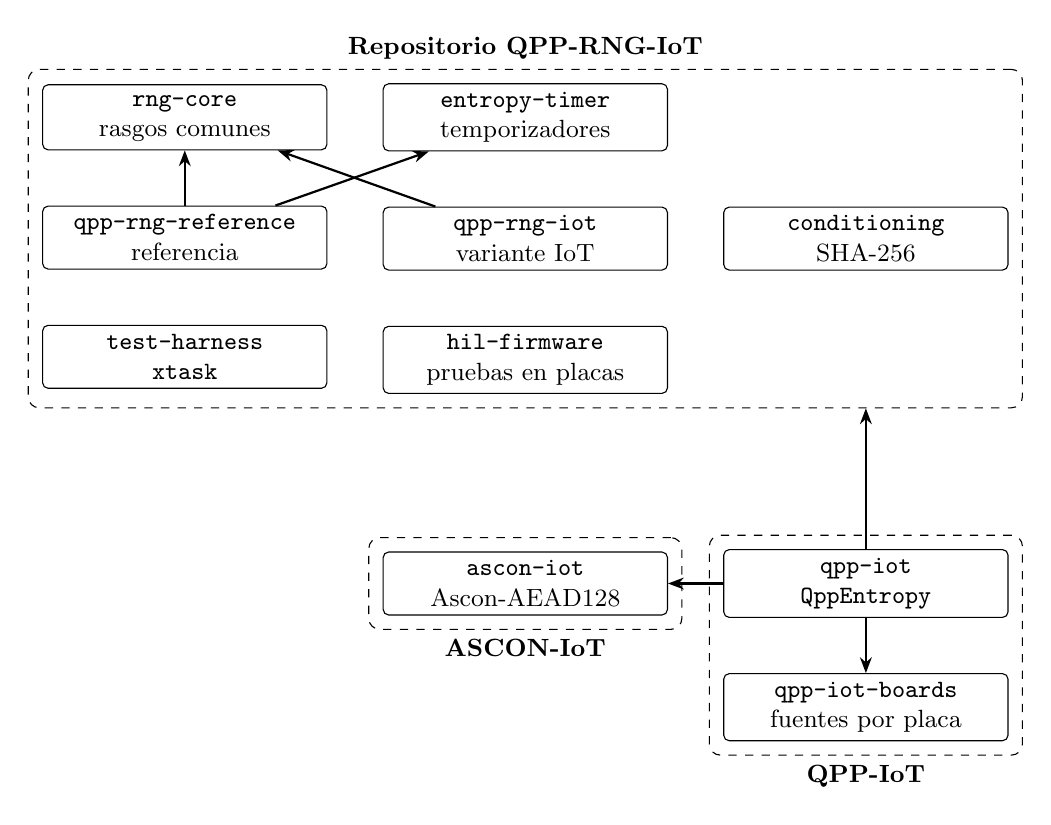
\begin{tikzpicture}[
    font=\small,
    caja/.style={draw, rounded corners=2pt, align=center, minimum height=8mm, inner sep=3pt, text width=34mm},
    repo/.style={draw, dashed, rounded corners=4pt, inner sep=5pt},
    flecha/.style={-{Stealth[length=2mm]}, thick}
]
\node[caja] (core) {\texttt{rng-core}\\rasgos comunes};
\node[caja, right=7mm of core] (timer) {\texttt{entropy-timer}\\temporizadores};
\node[caja, below=7mm of core] (ref) {\texttt{qpp-rng-reference}\\referencia};
\node[caja, below=7mm of timer] (iot) {\texttt{qpp-rng-iot}\\variante IoT};
\node[caja, right=7mm of iot] (cond) {\texttt{conditioning}\\SHA-256};
\node[caja, below=7mm of ref] (harness) {\texttt{test-harness}\\\texttt{xtask}};
\node[caja, below=7mm of iot] (hil) {\texttt{hil-firmware}\\pruebas en placas};
\node[repo, fit=(core)(timer)(ref)(iot)(cond)(harness)(hil), label={[font=\small\bfseries]above:Repositorio QPP-RNG-IoT}] (r1) {};

\node[caja, below=20mm of hil] (ascon) {\texttt{ascon-iot}\\Ascon-AEAD128};
\node[repo, fit=(ascon), label={[font=\small\bfseries]below:ASCON-IoT}] (r2) {};

\node[caja, right=7mm of ascon] (fachada) {\texttt{qpp-iot}\\\texttt{QppEntropy}};
\node[caja, below=7mm of fachada] (boards) {\texttt{qpp-iot-boards}\\fuentes por placa};
\node[repo, fit=(fachada)(boards), label={[font=\small\bfseries]below:QPP-IoT}] (r3) {};

\draw[flecha] (ref) -- (core);
\draw[flecha] (ref) -- (timer);
\draw[flecha] (iot) -- (core);
\draw[flecha] (fachada) -- (ascon);
\draw[flecha] (fachada.north) -- (fachada.north |- r1.south);
\draw[flecha] (fachada) -- (boards);
\end{tikzpicture}
\caption{Repositorios y \textit{crates} de la solución. Las flechas indican las principales dependencias.}
\label{fig:arquitectura}
\end{figure}

La Tabla~\ref{tab:crates} describe cada componente. Todos los que forman parte del camino de generación, es decir, todos salvo el arnés, el orquestador y los ejecutables de medición y de pruebas, compilan sin la biblioteca estándar y sin memoria dinámica.

\begin{table}[H]
\centering
\caption{Componentes de la solución}
\label{tab:crates}
\begin{tabularx}{\textwidth}{@{}L{0.30\textwidth}Y@{}}
\toprule
\textbf{Componente} & \textbf{Responsabilidad} \\
\midrule
\texttt{rng-core} & Rasgo \texttt{QppRngSource}, que extiende \texttt{rand\_core::Rng} con diagnósticos internos del último byte generado. \\
\texttt{entropy-timer} & Lectura del contador de alta resolución de cada plataforma mediante rutinas en C, y calibración de su resolución real. \\
\texttt{qpp-rng-reference} & Implementación fiel de QPP-RNG según Vrana et al.\ \cite{Vrana2025RawEvaluation}. \\
\texttt{qpp-rng-iot} & Variante para microcontroladores: fuente física independiente, pruebas de salud continuas, generación de permutaciones de bajo costo. \\
\texttt{conditioning} & Acondicionador SHA-256 con compresión 2:1. \\
\texttt{qpp-rng-firmware} & Un ejecutable por candidato, para medir la huella de cada uno por separado. \\
\texttt{test-harness} & Arnés de evaluación: \texttt{candidates}, \texttt{stats}, \texttt{bench}, \texttt{footprint}, \texttt{differential} y \texttt{report}. \\
\texttt{xtask} & Orquestador que ejecuta la comparación completa (\texttt{cargo xtask compare}). \\
\texttt{hil-firmware} & \textit{Firmware} de prueba para AVR, nRF52840 y ESP32, y herramientas de captura y análisis en el anfitrión. \\
\texttt{ascon-iot} & Ascon-AEAD128 (NIST SP 800-232) sobre la implementación de RustCrypto, con generación de claves y \textit{nonces} desde cualquier \texttt{rand\_core::Rng}. \\
\texttt{qpp-iot}, \texttt{qpp-iot-boards} & Fachada \texttt{QppEntropy} (fuente $\rightarrow$ QPP-RNG $\rightarrow$ SHA-256 $\rightarrow$ \texttt{Rng}) y una fuente física por placa. \\
\bottomrule
\end{tabularx}
\end{table}

\section{Rasgos comunes}

Los generadores de referencia y el acondicionador implementan el rasgo \texttt{Rng} del ecosistema \texttt{rand\_core} (versión 0.10), de modo que pueden usarse en cualquier librería de Rust que reciba un generador, incluida \texttt{ascon-iot}. La variante IoT implementa \texttt{TryRng} y se adapta a \texttt{Rng} mediante un envoltorio, como se describe más adelante. Sobre ese rasgo, \texttt{rng-core} define \texttt{QppRngSource}, que agrega una sola operación: \texttt{diagnostics()}, la cual expone el ancho de la permutación en bits, el último valor de $n_p$ y la última medición de tiempo. El arnés usa estos diagnósticos para reconstruir el comportamiento interno del generador sin modificar su camino de ejecución. Como ninguno de los dos rasgos tiene métodos genéricos, ambos admiten objetos de rasgo (\texttt{Box<dyn QppRngSource>}), lo que permite que el arnés recorra una lista heterogénea de candidatos.

Ningún generador implementa todavía el rasgo marcador \texttt{rand\_core::CryptoRng}. Ese marcador es una afirmación de seguridad hacia el código que lo consume y se reservó para cuando cada variante supere todas las pruebas de validación.

\section{Temporizadores de alta resolución}

El \textit{crate} \texttt{entropy-timer} encapsula, detrás del rasgo \texttt{HighResTimer}, el contador más barato y de mayor resolución que ofrece cada plataforma (Tabla~\ref{tab:temporizadores}). La lectura se realiza en C, con una rutina por plataforma que se selecciona en tiempo de compilación, de modo que el binario contiene exactamente una.

\begin{table}[H]
\centering
\caption{Contadores utilizados por plataforma}
\label{tab:temporizadores}
\begin{tabularx}{\textwidth}{@{}L{0.30\textwidth}Y@{}}
\toprule
\textbf{Plataforma} & \textbf{Contador} \\
\midrule
Windows & \texttt{QueryPerformanceCounter} \\
macOS en Apple Silicon & \texttt{mach\_absolute\_time} \\
Linux o macOS en x86 & \texttt{RDTSC} si el TSC es invariante; si no, \texttt{clock\_gettime} \\
Linux en ARM64 (Raspberry Pi 4) & Registro \texttt{CNTVCT\_EL0} del temporizador genérico (54 MHz en la Pi 4) \\
Linux en ARM32 & Contador de ciclos de la PMU, con respaldo a \texttt{clock\_gettime} \\
ESP32 (Xtensa LX6) & Registro especial \texttt{CCOUNT}, contador de ciclos de la CPU \\
AVR (ATmega328P, ATmega2560) & Timer1 sin preescalador, extendido a 32 bits por la interrupción de desbordamiento \\
Cortex-M (nRF52840) & \texttt{CYCCNT} de la unidad DWT \\
Otros sistemas Unix & \texttt{clock\_gettime(CLOCK\_MONOTONIC)} \\
\bottomrule
\end{tabularx}
\end{table}

\paragraph{Resolución adaptativa.} El artículo de referencia presenta como una de sus contribuciones un mecanismo de resolución de reloj adaptativa, que compensa las distintas granularidades de los temporizadores \cite{Vrana2025RawEvaluation}. La normalización que describe es
\begin{equation}
    \delta = \left\lfloor \frac{\Delta t}{k} \right\rfloor \bmod 256,
    \label{eq:normalizacion}
\end{equation}
donde $\Delta t$ es la diferencia entre dos lecturas del contador y $k$ es su resolución nativa. Una primera versión fijó $k$ como una constante por plataforma, y falló en la práctica: en un computador con Windows, la constante ($k = 100$, pensada para nanosegundos) se aplicaba a diferencias de ticks de \texttt{QueryPerformanceCounter}. En el equipo evaluado ese contador avanza a 10 MHz, de modo que un ciclo de aproximadamente 1 \textmu s equivale a unos 11 ticks y el cociente resultaba casi siempre cero, con lo que la salida colapsó sobre un único byte dominante. No se descarta que la granularidad efectiva del contador varíe entre equipos, pues una misma interfaz del sistema operativo puede estar respaldada por contadores físicos distintos. Por ello, la implementación mide $k$ empíricamente al construir el generador: toma 256 pares de lecturas consecutivas, tras un breve calentamiento, y usa la menor diferencia no nula, acotada al intervalo $[1, 255]$. Solo si el contador no avanza durante la calibración recurre a la constante nominal. En la Raspberry Pi 4 y en el computador con Windows, la calibración produjo $k = 1$, frente a valores nominales de 34 y 100.

\section{Implementación de referencia de QPP-RNG}
\label{sec:referencia}

\subsection{Mecanismo}

El \textit{crate} \texttt{qpp-rng-reference} implementa el generador descrito por Vrana, Lou y Kuang \cite{Vrana2025RawEvaluation}. El generador mantiene una semilla de 128 bits, $s$, y repite el siguiente ciclo de convergencia (Figura~\ref{fig:ciclo_referencia}):

\begin{enumerate}
    \item Se reinicializa el generador interno $P$ con la semilla $s$.
    \item Partiendo de la permutación identidad de un arreglo de $N$ elementos, se genera repetidamente un \textit{pad} de permutación con el algoritmo de Fisher--Yates \cite{Durstenfeld1964Algorithm235}, usando $P$, y se compone con el estado actual, hasta que el estado vuelve a ser la identidad. El número de \textit{pads} generados es $n_p$.
    \item Se mide con el temporizador el tiempo $\Delta t$ de todo el ciclo, se normaliza según la Ecuación~\eqref{eq:normalizacion} y se incorpora a la semilla: $s \leftarrow (s \ll 8) \,\|\, \delta$.
    \item El valor crudo del ciclo es $n_p \bmod 256$.
\end{enumerate}

Para $N = 5$, el valor por defecto del artículo, $\log_2 5! \approx 6.9$ bits, menos de un byte. Por ello, el artículo prescribe repetir el ciclo $m \geq 4$ veces por byte de salida. La configuración por defecto usa $m = 5$.

\begin{figure}[H]
\centering
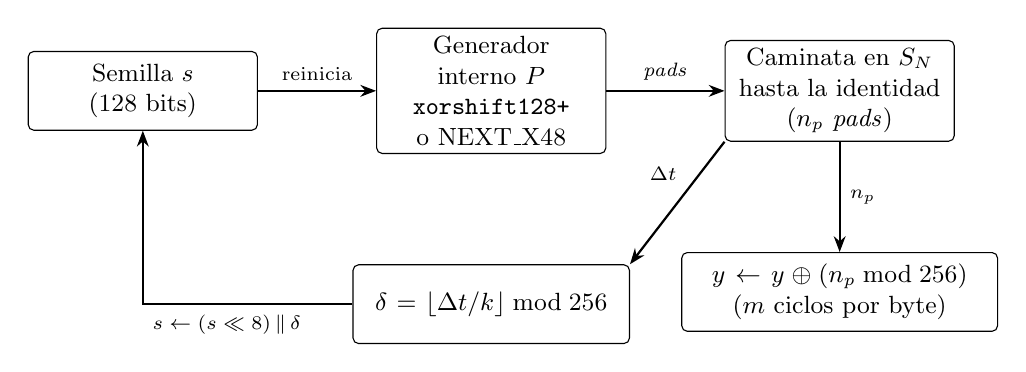
\begin{tikzpicture}[
    font=\small,
    caja/.style={draw, rounded corners=2pt, align=center, minimum height=10mm, inner sep=3pt, text width=27mm},
    etiqueta/.style={font=\scriptsize},
    flecha/.style={-{Stealth[length=2mm]}, thick}
]
\node[caja] (seed) {Semilla $s$\\(128 bits)};
\node[caja, right=15mm of seed] (prng) {Generador interno $P$\\\texttt{xorshift128+}\\o NEXT\_X48};
\node[caja, right=15mm of prng] (walk) {Caminata en $S_N$\\hasta la identidad\\($n_p$ \textit{pads})};
\node[caja, below=14mm of walk, text width=38mm] (out) {$y \leftarrow y \oplus (n_p \bmod 256)$\\($m$ ciclos por byte)};
\node[caja, below=14mm of prng, text width=33mm] (dt) {$\delta = \lfloor \Delta t / k \rfloor \bmod 256$};
\draw[flecha] (seed) -- node[etiqueta, above]{reinicia} (prng);
\draw[flecha] (prng) -- node[etiqueta, above]{\textit{pads}} (walk);
\draw[flecha] (walk) -- node[etiqueta, right]{$n_p$} (out);
\draw[flecha] (walk.south west) -- node[etiqueta, above left, pos=0.4]{$\Delta t$} (dt.north east);
\draw[flecha] (dt.west) -| node[etiqueta, below, pos=0.3]{$s \leftarrow (s \ll 8)\,\|\,\delta$} (seed.south);
\end{tikzpicture}
\caption{Ciclo de convergencia de la implementación de referencia.}
\label{fig:ciclo_referencia}
\end{figure}

El Listado~\ref{lst:ciclo} muestra el núcleo del ciclo de convergencia, en una versión simplificada del código.

\begin{lstlisting}[language=Rust, caption={Ciclo de convergencia de la referencia (simplificado)}, label={lst:ciclo}]
fn run_convergence_cycle(&mut self) -> (u64, u64) {
    self.prng.seed(self.seed);
    let identity: [u8; N] = core::array::from_fn(|i| i as u8);
    let mut current = identity;
    let mut n_p: u64 = 0;
    let t0 = self.timer.tick();
    loop {
        n_p += 1;
        let pad = generate_permutation::<P, N>(&mut self.prng);
        current = apply_permutation(&current, &pad);
        core::hint::black_box(&current); // impide colapsar el bucle
        if current == identity { break; }
    }
    let t1 = self.timer.tick();
    (n_p, t1.wrapping_sub(t0))
}
\end{lstlisting}

\subsection{Decisiones de fidelidad}

El artículo describe el mecanismo en prosa, con algunas fórmulas, pero no publica pseudocódigo ni código fuente. Las decisiones que deja abiertas se tomaron así:

\begin{itemize}
    \item \textbf{Caminata de convergencia.} Se implementó como una caminata aleatoria en el grupo simétrico $S_N$: desde la identidad, se multiplica a la derecha por permutaciones independientes y uniformes hasta volver a la identidad. Como el producto de un estado cualquiera por una permutación uniforme independiente es uniforme, cada paso regresa a la identidad con probabilidad $1/N!$, y $n_p$ sigue una distribución geométrica de parámetro $q = 1/N!$, con media $N!$. Esto es coherente con la contabilidad de entropía $e = \log_2 N!$ del artículo.
    \item \textbf{Combinación del sobremuestreo.} El artículo no especifica cómo se combinan los $m$ ciclos por byte. Se eligió el XOR de los $m$ valores $n_p \bmod 256$, porque el XOR de muestras independientes es al menos tan impredecible como cualquiera de ellas.
    \item \textbf{Evolución de la semilla.} El desplazamiento $s \leftarrow (s \ll 8) + \delta$ se aplicó a la semilla completa de 128 bits, como un registro de desplazamiento único, y el generador interno se reinicia antes de \emph{cada} ciclo, de acuerdo con la propiedad de independencia que describe el artículo.
    \item \textbf{Generadores internos.} \texttt{Xorshift128Plus} sigue la construcción de Vigna \cite{Vigna2017FurtherGenerators}. \texttt{NextX48} sigue el generador congruencial lineal de 48 bits de \texttt{java.util.Random} (multiplicador \texttt{0x5DEECE66D}, incremento \texttt{0xB}), que el artículo cita para NEXT\_X48. Los índices de Fisher--Yates se obtienen con la reducción de Lemire sobre 64 bits \cite{Lemire2019FastInterval}.
\end{itemize}

\subsection{Sensibilidad a la optimización del compilador}

La fuente de entropía de la referencia es el tiempo de ejecución de su propio bucle, de modo que un compilador optimizador puede destruirla. Esto se comprobó experimentalmente: con el perfil de compilación de la librería (optimización completa, LTO y una sola unidad de generación de código), el compilador demostró que los efectos del bucle sobre la memoria eran locales, lo redujo a una ejecución casi sin variación temporal y el registro de la semilla quedó atrapado en un punto fijo. En una muestra de 5\,000 bytes, un único valor apareció en más del 70\,\% de las posiciones. El artículo evita este problema compilando con \texttt{-O0} \cite{Vrana2025RawEvaluation}. En la librería se aplicaron dos medidas: se fijó el nivel de optimización 0 para \texttt{qpp-rng-reference} y \texttt{entropy-timer} en todos los perfiles, y se insertó una barrera \texttt{core::hint::black\_box} en cada iteración del bucle. Una prueba de regresión verifica, con el temporizador real, que ningún valor ocupe más del 10\,\% de una muestra de 2\,000 bytes.

\subsection{Sesgo estructural de la extracción}
\label{sec:sesgo}

La extracción $n_p \bmod 256$ tiene un sesgo que no depende del temporizador. Como $n_p \sim \text{Geom}(q)$ con $q = 1/N!$, la probabilidad de que el bit 7 del valor extraído valga 1 es
\begin{equation}
    p_7 = \Pr\left[(n_p \bmod 256) \geq 128\right] = \frac{r^{127} - r^{255}}{1 - r^{256}}, \qquad r = 1 - q.
    \label{eq:sesgo_bit7}
\end{equation}
Para $N = 5$, la media de $n_p$ es 120, menor que 256: la cola geométrica decae antes de dar una vuelta completa al módulo, y $p_7 = 0.2573$. El XOR de $m$ valores independientes reduce el sesgo de forma geométrica:
\begin{equation}
    \Pr[\text{bit 7 del XOR} = 1] = \frac{1}{2} - \frac{1}{2}\,(1 - 2p_7)^m.
    \label{eq:sesgo_xor}
\end{equation}
Con $m = 5$, la probabilidad resultante es $0.48654$, todavía detectable con un millón de bytes. La Tabla~\ref{tab:sesgo} resume los valores exactos. Este análisis motivó dos decisiones de diseño: acondicionar siempre la salida cruda antes de usarla como material de clave (Sección~\ref{sec:acondicionamiento}) y usar $N = 6$ en la variante IoT (Sección~\ref{sec:variante_iot}).

\begin{table}[H]
\centering
\caption{Probabilidad exacta de que el bit 7 valga 1, según las Ecuaciones~\eqref{eq:sesgo_bit7} y~\eqref{eq:sesgo_xor}}
\label{tab:sesgo}
\begin{tabular}{@{}cccc@{}}
\toprule
$N$ & Media de $n_p$ & Un ciclo & XOR de $m$ ciclos \\
\midrule
5 & 120 & 0.2573 & 0.4723 ($m = 4$), 0.48654 ($m = 5$) \\
6 & 720 & 0.4563 & 0.49997 ($m = 4$) \\
\bottomrule
\end{tabular}
\end{table}

\section{Acondicionamiento con SHA-256}
\label{sec:acondicionamiento}

El \textit{crate} \texttt{conditioning} implementa un componente de acondicionamiento en el sentido de SP 800-90B: \texttt{Sha256Conditioner} acumula 64 bytes crudos de la fuente que envuelve, los comprime con SHA-256 \cite{NIST2015SecureHashStandard} y entrega los 32 bytes del resumen antes de solicitar el siguiente bloque. La relación de compresión 2:1 (512 bits de entrada nominales para 256 bits de salida) busca dejar holgura sobre el margen habitual de 64 bits por encima del tamaño de la salida ($256 + 64 = 320$ bits). En la variante IoT, cada byte crudo se produce a partir de muestras físicas a las que se acreditan al menos 8 bits de min-entropía. Esa cifra es un límite superior de la entropía que llega al acondicionador, no una garantía, porque la caminata de QPP-RNG es una transformación determinista que no puede aumentar la entropía y podría reducirla (en particular, la semilla de 64 bits se reduce a 32 bits antes de cada caminata). Demostrar una cota inferior requiere analizar la conservación de entropía a través de la caminata, lo que se deja como trabajo futuro. En la referencia ejecutada en computadores, donde cada ciclo aporta unos 1.9 bits frescos por byte (experimento E4), 64 bytes crudos no alcanzan los 256 bits, por lo que el acondicionamiento no basta para respaldar su uso criptográfico.

El acondicionador se mantuvo en un \textit{crate} propio por la misma razón que separa la referencia de la variante IoT: la fuente cruda sigue disponible sin modificaciones para su evaluación y el arnés puede registrar cada candidato en forma cruda y acondicionada. Su documentación advierte que no debe estimarse la entropía de la salida acondicionada con \texttt{ea\_non\_iid}: un buen \textit{hash} borra los patrones de corto alcance que esos estimadores buscan, en ambas direcciones.

\section{Variante para microcontroladores: \texttt{qpp-rng-iot}}
\label{sec:variante_iot}

\subsection{Motivación}

El experimento E1 (Sección~\ref{sec:res_determinismo}) mostró que la referencia no tiene entropía en los cuatro microcontroladores: desde un reinicio, cada placa reproduce exactamente la misma traza $(n_p, \Delta t)$. En un núcleo sin sistema operativo y sin otros maestros de bus, cada instrucción tarda un número de ciclos que depende solo del estado del propio programa y el temporizador cuenta el mismo reloj que la CPU, de modo que $\Delta t$ es una función determinística de la semilla. La caché de la Flash de la ESP32 no cambia esta conclusión: su contenido también es una función determinística del programa ejecutado desde el reinicio. La variante IoT conserva la estructura de QPP-RNG, pero cambia la fuente de entropía y, de paso, el costo de cómputo. La Tabla~\ref{tab:cambios_iot} resume las diferencias.

\begin{table}[H]
\centering
\caption{Diferencias entre la referencia y la variante IoT}
\label{tab:cambios_iot}
\begin{tabularx}{\textwidth}{@{}L{0.17\textwidth}L{0.25\textwidth}L{0.27\textwidth}Y@{}}
\toprule
\textbf{Aspecto} & \textbf{Referencia} & \textbf{Variante IoT} & \textbf{Motivo} \\
\midrule
Fuente & Tiempo del propio bucle, medido con el reloj de la CPU & Rasgo \texttt{JitterSource}: un oscilador independiente medido en ciclos de la CPU & El tiempo del propio bucle es determinístico en microcontroladores \\
Pruebas de salud & Ninguna & RCT y APT de SP 800-90B sobre cada muestra & Una fuente degradada debe fallar de forma explícita \\
Generador de \textit{pads} & \texttt{xorshift128+}, semilla de 128 bits, Lemire de 64 bits & \texttt{xorshift32} sembrado con \texttt{fmix32}, Lemire de 8 bits con tabla de umbrales & La aritmética de 64 y 128 bits es costosa en un núcleo de 8 bits \\
Caminata & Generar \textit{pad}, componer en un arreglo nuevo, comparar & Intercambios de Fisher--Yates aplicados sobre el estado, con salida temprana & La misma caminata con la mitad del tráfico de memoria \\
$N$ & 5 (media de $n_p$: 120) & 6 (media: 720) & Elimina el sesgo estructural (Tabla~\ref{tab:sesgo}) \\
Contabilidad & Una medición por ciclo, 5 ciclos por byte & $\lceil 8/H \rceil$ muestras por byte, repartidas en 4 caminatas fijas & Separa ``suficiente entropía'' de ``suficiente cómputo'' \\
Interfaz & \texttt{Rng} (infalible) & \texttt{TryRng<Error = HealthError>} & Los errores son reportables en el dispositivo \\
\bottomrule
\end{tabularx}
\end{table}

\subsection{Fuente de entropía}

El rasgo \texttt{JitterSource} tiene un único método, \texttt{sample()}, que bloquea hasta la siguiente medición y la retorna como un entero de 32 bits con la entropía en los bits de menor orden. La documentación del rasgo establece la condición que una implementación debe cumplir: medir algo cuyo reloj sea físicamente independiente de la CPU (un oscilador RC separado, un oscilador de anillo o un evento externo), en unidades de un contador síncrono con la CPU. Medir trabajo de la propia CPU con un contador de la propia CPU no es una implementación válida en estos dispositivos.

\subsection{Pruebas de salud continuas}

Cada muestra cruda pasa por las dos pruebas continuas de SP 800-90B \cite{Turan2018RecommendationGeneration}: la prueba de conteo de repeticiones (RCT) y la prueba de proporción adaptativa (APT). Ambas se configuran a partir de la min-entropía $H$ acreditada a la fuente, con una tasa de falsos positivos $\alpha = 2^{-20}$:
\begin{equation}
    C_{\text{RCT}} = 1 + \left\lceil \frac{20}{H} \right\rceil, \qquad
    C_{\text{APT}} = 1 + \operatorname{CRITBINOM}\!\left(W,\, 2^{-H},\, 1 - 2^{-20}\right), \quad W = 512.
\end{equation}
La RCT falla si un mismo valor se repite $C_{\text{RCT}}$ veces seguidas. La APT falla si, en una ventana de $W$ muestras, el primer valor aparece $C_{\text{APT}}$ veces o más. Para $H = 1$, los umbrales son 21 y 311. Para $H = 4$, 6 y 62, el mayor valor tabulado: un valor acreditado mayor que 4 se trata como 4. Una falla se reporta como \texttt{HealthError} en lugar de producir bytes de baja entropía en silencio. Estas pruebas detectan una fuente atascada o degradada, pero no pueden detectar una fuente que varía de forma completamente determinística, como la referencia en un microcontrolador: ese modo de falla tiene que eliminarse en el diseño, eligiendo una fuente físicamente independiente.

\subsection{Contabilidad de entropía}

En la referencia, una medición de tiempo equivale a un ciclo de convergencia, de modo que una fuente pobre obliga a ejecutar muchas caminatas costosas por byte. En la variante IoT, ambas cantidades se separan. El número de muestras por byte se deriva de la min-entropía acreditada, de modo que cada byte quede respaldado por al menos 8 bits acreditados:
\begin{equation}
    \text{muestras por caminata} = \max\!\left(1,\; \left\lceil \frac{\lceil 8 / H \rceil}{4} \right\rceil \right),
\end{equation}
mientras que el número de caminatas por byte se fija en 4, lo justo para aplanar el sesgo de la extracción con $N = 6$ (Tabla~\ref{tab:sesgo}). Con $H = 1$ (AVR), cada byte absorbe 8 muestras, con $H = 4$ (RNG del nRF52840 o de la ESP32), 4. Cada muestra se incorpora a una semilla de 64 bits como $s \leftarrow (s \ll 8) \oplus x$. Antes del primer byte, el generador absorbe 8 muestras adicionales para que la salida inicial no dependa de la semilla nula.

\subsection{Generación de permutaciones de bajo costo}

En el ATmega2560, la referencia gasta en promedio unos 1\,090 ciclos por índice de Fisher--Yates, casi todos en aritmética de 64 y 128 bits emulada por un núcleo de 8 bits. La variante IoT reduce ese costo en tres pasos:

\begin{itemize}
    \item \textbf{Generador más estrecho.} El generador de \textit{pads} no es la fuente de entropía; solamente expande la semilla en índices. Por eso se reemplazó \texttt{xorshift128+} por \texttt{xorshift32} de Marsaglia \cite{Marsaglia2003XorshiftRNGs}, sembrado con la función de mezcla \texttt{fmix32} aplicada a la semilla de 64 bits. Un paso de \texttt{xorshift32} produce cuatro bytes.
    \item \textbf{Reducción de Lemire de 8 bits.} Para $N \leq 8$, cada índice está acotado por 8, de modo que un byte aleatorio y una multiplicación de $8 \times 8 \rightarrow 16$ bits (una sola instrucción \texttt{mul} en AVR) bastan para una reducción de Lemire exactamente insesgada \cite{Lemire2019FastInterval}. El umbral de rechazo $256 \bmod b$ se toma de una tabla, porque AVR no tiene instrucción de división y la operación módulo en software consumía cerca del 85\,\% del tiempo de la caminata.
    \item \textbf{Caminata fusionada.} En lugar de generar un \textit{pad} completo y luego componerlo en un arreglo nuevo, los intercambios de Fisher--Yates se aplican directamente sobre el estado, y la comparación con la identidad termina en la primera diferencia. Una prueba unitaria verifica que esta caminata es la misma, con los mismos índices, que la composición explícita.
\end{itemize}

\subsection{Interfaz}

\texttt{QppRngIot} implementa \texttt{TryRng<Error = HealthError>}, de modo que una falla de salud es un valor de retorno. Para las interfaces que exigen un generador infalible, el envoltorio \texttt{PanicOnHealthFailure} convierte la falla en un pánico e implementa \texttt{QppRngSource}. La salida de la variante IoT es salida cruda de una fuente de entropía y, al igual que la de la referencia, debe acondicionarse antes de usarse como material de clave.

\section{Fuentes físicas por plataforma}
\label{sec:fuentes}

\paragraph{AVR: perro guardián contra Timer1.} El perro guardián de los ATmega se alimenta de un oscilador RC interno de 128 kHz, independiente del cristal de 16 MHz que alimenta la CPU y el Timer1. La fuente configura el perro guardián en modo de solo interrupción con su periodo más corto (alrededor de 16 ms) y, en cada interrupción, guarda la lectura del Timer1 en un búfer circular de 16 posiciones. La muestra es la diferencia entre dos marcas de tiempo, es decir, el periodo del oscilador RC medido en ciclos del cristal. El ruido de fase térmico del oscilador RC se acumula durante el periodo y aparece en los bits bajos de la medición.

\paragraph{nRF52840: generador en hardware.} El nRF52840 incluye un periférico RNG basado en ruido térmico, con corrección de sesgo. Se evaluó también una fuente análoga a la de AVR (el RTC alimentado por el oscilador LFRC de 32.768 kHz contra el contador de ciclos), pero su min-entropía resultó baja (Sección~\ref{sec:res_fuentes}), y se prefirió el periférico RNG, que la variante IoT usa como \texttt{JitterSource}.

\paragraph{ESP32: generador en hardware con su fuente de ruido activa.} La ESP32 también incluye un periférico RNG. Según la documentación del fabricante, su salida solo es verdaderamente aleatoria mientras está activa alguna fuente de ruido física, la radio o el ruido del ADC de aproximaciones sucesivas (SAR); con ambas apagadas, debe considerarse pseudoaleatoria. Como los \textit{firmwares} de este trabajo no usan la radio, la fuente de la ESP32 toma posesión del ADC1 al construirse y deja la fuente de ruido del ADC activada durante toda la ejecución, de modo que la precondición queda garantizada por el tipo y no por la disciplina de quien integra la librería. Cada muestra es el byte bajo de una palabra del RNG. Se evaluó también una fuente análoga a la de AVR: el reloj lento del dominio RTC, un oscilador RC de unos 156 kHz, cuyo periodo acumulado durante 256 ciclos mide en ciclos del cristal de 40 MHz la unidad de calibración del grupo de temporizadores 0. Esa fuente resultó utilizable, pero más débil que el RNG (Sección~\ref{sec:res_fuentes}), y no se usa. El \textit{firmware} se ejecuta en el núcleo 0, con el núcleo 1 detenido y la radio apagada.

\section{Arnés de evaluación}
\label{sec:arnes}

El arnés se construyó antes de cualquier optimización, con una premisa: una variante más rápida que pierde entropía de forma silenciosa es peor que no tener variante. Su núcleo es el registro \texttt{candidates}, una lista de todas las configuraciones bajo prueba. Hoy contiene cuatro: la referencia con \texttt{xorshift128+} y con NEXT\_X48, cada una en forma cruda y acondicionada con SHA-256. Cinco \textit{crates} responden, cada uno, a una pregunta sobre todos los candidatos, y escriben su respuesta en JSON:

\begin{itemize}
    \item \texttt{stats} genera muestras de al menos 1\,000\,000 de bytes y ejecuta el nivel 1 (cinco pruebas nativas, con funciones matemáticas verificadas contra los ejemplos resueltos de SP 800-22) y el nivel 2 (ENT, \texttt{ea\_iid}, \texttt{ea\_non\_iid} y \texttt{assess}). Para SP 800-22, el número de flujos se deriva del tamaño real de la muestra (8 flujos de $10^6$ bits por cada megabyte).
    \item \texttt{bench} mide con \textit{Criterion} el rendimiento sostenido, la latencia por llamada y el tiempo hasta el primer byte.
    \item \texttt{footprint} mide ciclos por llamada, y el tamaño de cada ejecutable de \texttt{qpp-rng-firmware} con \texttt{cargo size} y \texttt{cargo bloat}. Hay un ejecutable por candidato para que el enlazador elimine el código de los demás.
    \item \texttt{differential} verifica el determinismo de cada configuración frente a un reloj simulado, la paridad de comportamiento entre candidatos y la ausencia de pánicos mediante \textit{proptest} para $N \in \{1, 2, 5, 6, 8\}$ con \texttt{xorshift128+} y $N \in \{1, 5, 6\}$ con NEXT\_X48.
    \item \texttt{report} une los resultados por nombre de candidato y genera una tabla comparativa en Markdown y CSV.
\end{itemize}

El orquestador \texttt{xtask} ejecuta la secuencia completa con \texttt{cargo xtask compare}. Varias fallas del propio arnés se encontraron al probarlo contra las herramientas reales y se corrigieron. Por ejemplo, el orden exacto de las seis respuestas que espera el menú interactivo de \texttt{assess}, la copia de las plantillas que necesita la prueba \textit{NonOverlappingTemplate} y la conservación del veredicto de las pruebas IID de \texttt{ea\_iid}, que antes se descartaba. La suite del espacio de trabajo consta de 118 pruebas, todas superadas, y una adicional que se ignora por defecto.

\section{\textit{Firmware} de pruebas sobre hardware}
\label{sec:hil}

El arnés del anfitrión no puede detectar el modo de falla principal de este trabajo porque la salida determinística de la referencia supera las pruebas estadísticas. Para eso se construyó un \textit{firmware} de pruebas para AVR, para el nRF52840 y para la ESP32 con tres modos seleccionados en tiempo de compilación (Tabla~\ref{tab:modos_hil}). Todos transmiten por UART a 115\,200 baudios una línea de encabezado que comienza con \texttt{QPPHIL}, seguida de registros formados por un byte de sincronización (\texttt{0xA5}) y dos enteros de 32 bits en orden \textit{little-endian}. El código común a todas las placas (el protocolo y el ciclo completo del modo IoT) vive en un \textit{crate} compartido. En la ESP32, la inicialización de relojes y de la UART se delega en \texttt{esp-hal}, y existe un cuarto modo que repite la captura de la fuente cruda con la fuente de ruido del ADC desactivada, como control.

\begin{table}[H]
\centering
\caption{Modos del \textit{firmware} de pruebas}
\label{tab:modos_hil}
\begin{tabularx}{\textwidth}{@{}L{0.20\textwidth}L{0.38\textwidth}Y@{}}
\toprule
\textbf{Modo} & \textbf{Registros transmitidos} & \textbf{Uso} \\
\midrule
Traza de referencia & $n_p$ y $\Delta t$ de cada ciclo de la referencia & Repetibilidad entre reinicios (E1) \\
Fuente cruda & Muestra de la fuente física (y palabra del RNG en el nRF52840 y en la ESP32) & Estimación con SP 800-90B (E2) \\
IoT & 4 bytes de salida de \texttt{qpp-rng-iot} y los ciclos que tomaron & Rendimiento y pruebas de la salida (E3) \\
\bottomrule
\end{tabularx}
\end{table}

En el anfitrión, un programa de captura abre el puerto serie (lo que reinicia una placa Arduino), valida el encabezado y la sincronización de cada registro y escribe los registros y un archivo de metadatos. Un registro solo se acepta si el byte que le sigue es el de sincronización del siguiente, y los rechazos se cuentan en los metadatos. Esta comprobación se añadió después de que, en la ESP32, se perdiera un byte en el enlace serie y un registro desplazado entrara en los datos (Sección~\ref{sec:res_fuentes}). Otro programa convierte los registros en flujos de bytes para las herramientas del NIST. Para las capturas largas se escribió un controlador que captura bloques de 20\,000 registros, reintenta un bloque fallido y se detiene ante una falla de las pruebas de salud.

\section{Cifrado autenticado: ASCON-IoT}
\label{sec:ascon_iot}

El \textit{crate} \texttt{ascon-iot} envuelve, sin modificar su comportamiento criptográfico, la implementación de ASCON-AEAD128 de RustCrypto \cite{RustCryptoAEADs}, fijada en una revisión específica. Expone cifrado y descifrado autenticados en el mismo búfer (sin memoria dinámica), con clave de 128 bits, \textit{nonce} de 128 bits y etiqueta de 128 bits, y dos funciones que obtienen material aleatorio de cualquier \texttt{rand\_core::Rng}: \texttt{generate\_key} y \texttt{generate\_random\_nonce}. El repositorio se mantiene desacoplado del generador, de modo que el cifrado pueda validarse contra los vectores oficiales sin que intervenga QPP-RNG. QPP-RNG solo aparece en una prueba de integración, que lo usa para producir la clave y el \textit{nonce}, cifra un mensaje con datos asociados y verifica el descifrado.

\section{Integración: QPP-IoT}
\label{sec:qpp_iot}

La fachada \texttt{qpp-iot} combina los dos repositorios anteriores en un solo tipo, \texttt{QppEntropy}, que construye la tubería completa de la Figura~\ref{fig:tuberia}. Quien la usa entrega una fuente física y la min-entropía acreditada por muestra, y recibe un \texttt{rand\_core::Rng} listo para generar claves y \textit{nonces}.

\begin{figure}[H]
\centering
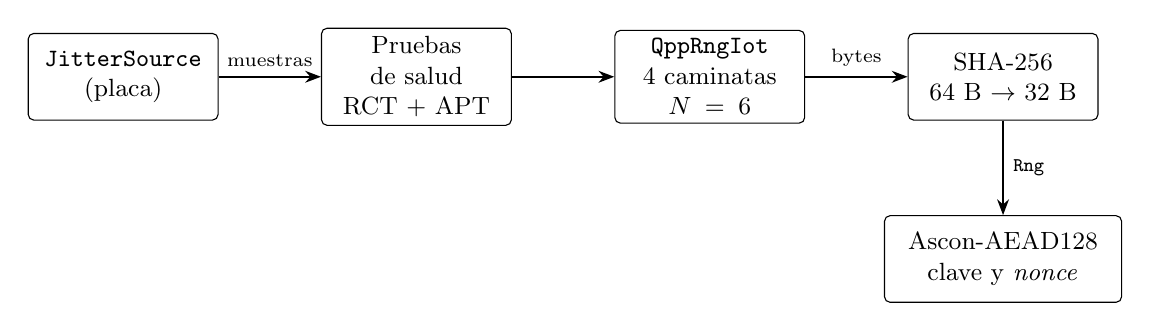
\begin{tikzpicture}[
    font=\small,
    caja/.style={draw, rounded corners=2pt, align=center, minimum height=11mm, inner sep=3pt, text width=22mm},
    etiqueta/.style={font=\scriptsize},
    flecha/.style={-{Stealth[length=2mm]}, thick}
]
\node[caja] (src) {\texttt{JitterSource}\\(placa)};
\node[caja, right=13mm of src] (health) {Pruebas de salud\\RCT + APT};
\node[caja, right=13mm of health] (qpp) {\texttt{QppRngIot}\\4 caminatas\\$N = 6$};
\node[caja, right=13mm of qpp] (sha) {SHA-256\\64 B $\rightarrow$ 32 B};
\node[caja, below=12mm of sha, text width=28mm] (ascon) {Ascon-AEAD128\\clave y \textit{nonce}};
\draw[flecha] (src) -- node[etiqueta, above]{muestras} (health);
\draw[flecha] (health) -- (qpp);
\draw[flecha] (qpp) -- node[etiqueta, above]{bytes} (sha);
\draw[flecha] (sha) -- node[etiqueta, right]{\texttt{Rng}} (ascon);
\end{tikzpicture}
\caption{Tubería de \texttt{QppEntropy}, desde la fuente física hasta Ascon-AEAD128.}
\label{fig:tuberia}
\end{figure}

El \textit{crate} \texttt{qpp-iot-boards} provee una fuente por placa, cada una detrás de una característica de compilación: \texttt{avr-wdt} (Arduino Uno, Nano y Mega 2560), \texttt{nrf52840}, \texttt{esp32} y \texttt{mock}, un generador determinístico \emph{sin entropía}, útil únicamente para probar la tubería en el anfitrión. Activar la característica de una placa al compilar para otra arquitectura produce un error de compilación. Como el acondicionador solo acepta una fuente infalible, \texttt{QppEntropy} usa el envoltorio que entra en pánico ante una falla de salud. Por ello, la configuración recomendada es \texttt{panic = \textquotedbl{}abort\textquotedbl{}} y el pánico debe tratarse como ``reiniciar y volver a sembrar'', nunca como ``continuar''.

En AVR, la tubería completa solo cabe en la memoria Flash si se usan las variantes compactas de los \textit{backends} de SHA-256 y ASCON, que se seleccionan con banderas de compilación (Sección~\ref{sec:res_huella}). Dado que una librería no puede fijar esas banderas por su cuenta, toda aplicación para AVR debe incluirlas en su configuración de compilación. El repositorio incluye un \textit{script} que lo hace y que falla si la imagen deja de caber. Si la aplicación también descifra, debe compilarse además con \texttt{opt-level = \textquotedbl{}z\textquotedbl{}}, de lo contrario, la imagen no cabe en un ATmega328P (Sección~\ref{sec:res_huella}). El repositorio incluye también el \textit{firmware} de la prueba de extremo a extremo y el \textit{script} que verifica su informe contra \texttt{ascon-c} (Sección~\ref{sec:res_e2e}).

%%=============================================================================
%% RESULTADOS
%%=============================================================================
\chapter{Resultados}
\label{cap:resultados}

Este capítulo presenta los resultados de los seis experimentos descritos en la Metodología (Capítulo~\ref{cap:metodologia}). Cada sección corresponde a un experimento. Salvo que se indique lo contrario, las estimaciones de min-entropía provienen de las herramientas oficiales del NIST (\texttt{ea\_non\_iid} y \texttt{ea\_iid}) y las pruebas de SP 800-22, de STS 2.1.2.

\section{E1: la referencia es determinística en microcontroladores}
\label{sec:res_determinismo}

La Tabla~\ref{tab:res_determinismo} resume las capturas de la traza $(n_p, \Delta t)$ de la referencia tras varios reinicios de cada placa, con la misma semilla.

\begin{table}[H]
\centering
\caption{Repetibilidad de la referencia entre reinicios}
\label{tab:res_determinismo}
\begin{tabularx}{\textwidth}{@{}Ycccrr@{}}
\toprule
\textbf{Plataforma} & \textbf{Reinicios} & \textbf{Registros} & \textbf{¿Idénticas?} & \textbf{Ciclos/\textit{pad}} & \textbf{B/s} \\
\midrule
Mega 2560 & 3 & 200--300 & sí, 100\,\% & 4\,374 & 5.95 \\
Nano & 2 & 300 & sí, 100\,\% & 4\,212 & 6.15 \\
Nano, referencia con \texttt{opt-level=\textquotedbl{}s\textquotedbl{}} & 2 & 300 & sí, 100\,\% & 4\,259 & 5.87 \\
nRF52840 & 3 & 2\,000 & sí, 100\,\% & 364 & 287 \\
Apple Silicon (control) & 3 & 64 B & no & -- & -- \\
\bottomrule
\end{tabularx}
\end{table}

En los tres microcontroladores, todas las capturas fueron idénticas bit a bit. La razón es que $\Delta t$ es una función determinística de los valores del generador interno (el número de \textit{pads}, los rechazos de la reducción de Lemire y las interrupciones de desbordamiento del temporizador), todos ellos funciones de la semilla, y la siguiente semilla es a su vez una función de $\Delta t$: no hay ruido independiente en ninguna parte del ciclo. La traza del Nano difiere de la del Mega (otra disposición del código produce otros conteos de ciclos), pero cada placa se repite a sí misma con exactitud. Compilar la referencia con optimización por tamaño en lugar de \texttt{-O0} no cambia el determinismo ni, de forma notable, la velocidad: en un núcleo de 8 bits domina la aritmética de 64 y 128 bits.

Las pruebas estadísticas no detectan esta falla. El byte bajo de $\Delta t$ en la traza del nRF52840 obtiene 4.93 bits por muestra con los estimadores MCV y \textit{t-tuple}, y la salida por defecto reconstruida a partir de la traza supera todas las pruebas de nivel 1 aplicables a 400 bytes. Solamente la comparación entre reinicios revela que la fuente no tiene entropía: la referencia, en estas plataformas, se comporta como un generador pseudoaleatorio cuya clave es la semilla fijada en tiempo de compilación.

\section{E2: fuentes físicas independientes}
\label{sec:res_fuentes}

La Tabla~\ref{tab:res_fuentes} resume la caracterización de las fuentes físicas. Las capturas de 20\,000 muestras tomaron unos 5.5 minutos por AVR y 35 segundos en el nRF52840; las de 1\,000\,001 muestras, del orden de 4.7 horas por AVR y 29 minutos en el nRF52840.

\begin{table}[H]
\centering
\caption{Caracterización de las fuentes físicas (min-entropía por muestra según \texttt{ea\_non\_iid})}
\label{tab:res_fuentes}
\small
\begin{tabularx}{\textwidth}{@{}Y R{0.16\textwidth} R{0.05\textwidth} R{0.10\textwidth} R{0.08\textwidth} R{0.07\textwidth} R{0.12\textwidth}@{}}
\toprule
\textbf{Fuente} & \textbf{Periodo medio (ciclos)} & \textbf{$\sigma$} & \textbf{Autocorr. lag 1} & \textbf{$H$ ($2 \cdot 10^4$)} & \textbf{$H$ ($10^6$)} & \textbf{Acreditado} \\
\midrule
Mega 2560, perro guardián & 271\,514 (16.97~ms) & 18.3 & 0.65 & 2.14 & \textbf{1.62} & 1 \\
Nano, perro guardián & 265\,950 (16.62~ms) & 45.1 & 0.69 & 2.98 & \textbf{2.24} & 1 \\
nRF52840, LFRC $\times 32$ & 111\,514 & 37.0 & $-0.91$ & 0.61 & \textbf{0.60} & no se usa \\
nRF52840, RNG en hardware & -- & -- & -- & 6.89 & \textbf{7.24} & 4 \\
\bottomrule
\end{tabularx}
\end{table}

En ambos AVR, el estimador determinante fue \textit{t-tuple}. Con un millón de muestras, ese estimador encuentra más estructura que con 20\,000, porque el periodo del perro guardián deriva lentamente (autocorrelación de 0.65 a 0.69), y los valores estimados bajaron entre 24 y 25\,\%. La Tabla~\ref{tab:res_estimadores_avr} detalla los estimadores. El valor acreditado de 1 bit por muestra sigue cubierto, con un margen de $1.6\times$ en el Mega y de $2.2\times$ en el Nano. Con 8 muestras por byte, cada byte de salida queda respaldado por al menos 12.9 bits estimados en el Mega y 17.9 en el Nano.

\begin{table}[H]
\centering
\caption{Estimadores de \texttt{ea\_non\_iid} sobre $10^6$ muestras del perro guardián (bits por muestra)}
\label{tab:res_estimadores_avr}
\begin{tabular}{@{}lcccccccc@{}}
\toprule
\textbf{Fuente} & \textbf{MCV} & \textbf{\textit{t-tuple}} & \textbf{LRS} & \textbf{MultiMCW} & \textbf{Lag} & \textbf{MultiMMC} & \textbf{LZ78Y} & \textbf{Estimado} \\
\midrule
Mega 2560 & 4.56 & \textbf{1.62} & 1.86 & 3.30 & 2.01 & 2.31 & 3.78 & \textbf{1.62} \\
Nano & 4.91 & \textbf{2.24} & 3.38 & 2.93 & 3.30 & 2.92 & 2.93 & \textbf{2.24} \\
\bottomrule
\end{tabular}
\end{table}

La fuente LFRC del nRF52840 presentó solo 42 valores distintos y una fuerte correlación negativa entre muestras consecutivas. El oscilador de 32.768 kHz es mucho más estable que el del perro guardián de AVR, y lo que varía es principalmente la cuantización de la lectura del contador del RTC: una marca de tiempo que llega tarde en un flanco llega temprano en el siguiente. Como el chip tiene un generador en hardware, esta fuente se descartó.

El periférico RNG del nRF52840, con un millón de muestras, obtuvo 7.24 bits por byte con \texttt{ea\_non\_iid} (MCV 7.88, \textit{t-tuple} 7.35, LRS 7.72, predictores entre 7.91 y 7.95; el valor determinante proviene de la evaluación por bits, multiplicada por 8) y superó todas las pruebas IID de \texttt{ea\_iid} (independencia por $\chi^2$, $p = 0.94$). Se le acreditaron 4 bits por byte, el mayor valor que cubre la tabla de umbrales de las pruebas de salud, con un margen de más de 3 bits.

Una segunda captura independiente de cada fuente difirió de la primera desde la primera muestra; para el RNG del nRF52840, hubo 79 coincidencias posicionales en 20\,000 muestras, frente a 78 esperadas por azar. Esta es exactamente la propiedad de la que carece la referencia. Como era de esperar, las muestras crudas fallan gravemente las pruebas de nivel 1 ($\chi^2 \approx 10^5$, correlación serial entre 0.4 y 0.65): son una fuente de ruido con deriva lenta, no bytes uniformes, y por eso el generador las procesa y acondiciona.

\section{E3: la variante IoT sobre hardware}
\label{sec:res_iot}

\subsection{Optimización del cómputo}

La Tabla~\ref{tab:res_optimizacion} muestra la evolución del costo de cómputo por byte en el ATmega2560, medida con una fuente sintética para aislar el cómputo de la espera por muestras.

\begin{table}[H]
\centering
\caption{Costo de cómputo por byte de salida en el ATmega2560}
\label{tab:res_optimizacion}
\begin{tabularx}{\textwidth}{@{}Xrr@{}}
\toprule
\textbf{Paso} & \textbf{Ciclos por byte} & \textbf{Mejora} \\
\midrule
Primera versión ($N = 6$, 8 caminatas por byte, $256 \bmod b$ por índice) & 10\,733\,218 & -- \\
Umbral de Lemire tomado de una tabla (AVR no tiene divisor) & 4\,585\,746 & $2.3\times$ \\
Generación y composición fusionadas, salida temprana & 2\,863\,887 & $1.6\times$ \\
4 caminatas por byte, 2 muestras por caminata & \textbf{1\,621\,365} & $1.8\times$ \\
\bottomrule
\end{tabularx}
\end{table}

En total, el cómputo por byte se redujo $6.6\times$. Por índice de Fisher--Yates, el costo pasó de unos 1\,090 ciclos en la referencia a unos 113 en la variante IoT ($9.7\times$), y por \textit{pad} se redujo cerca de $7.8\times$, aunque cada \textit{pad} de la variante IoT tiene un índice más ($N = 6$). Con 1.62 millones de ciclos (101 ms) por byte frente a 8 muestras del perro guardián por byte ($8 \times 17 = 136$ ms), el generador en AVR quedó limitado por la fuente y no por el cómputo: la caminata termina mientras la interrupción del perro guardián todavía está acumulando las siguientes muestras.

\subsection{Divergencia, rendimiento y huella}

La Tabla~\ref{tab:res_iot_hw} resume la ejecución de la variante IoT en las tres placas. En los tres casos, la salida difirió entre reinicios y no hubo fallas de las pruebas de salud.

\begin{table}[H]
\centering
\caption{Variante IoT sobre hardware}
\label{tab:res_iot_hw}
\begin{tabularx}{\textwidth}{@{}L{0.15\textwidth}>{\raggedright\arraybackslash}XL{0.17\textwidth}rcr@{}}
\toprule
\textbf{Placa} & \textbf{Entre reinicios (coincidencias)} & \textbf{Bytes (tiempo)} & \textbf{B/s} & \textbf{Fallas de salud} & \textbf{Flash} \\
\midrule
Mega 2560 & distintas, 0/40 & 10\,000 (22.6 min) & 7.36 & 0 & 6\,470 B \\
Nano & distintas, 0/40 & 10\,000 (22.2 min) & 7.52 & 0 & 6\,330 B \\
nRF52840 & distintas, 0/200 & 50\,000 (8.2 min) & 101 & 0 & 2\,940 B \\
\bottomrule
\end{tabularx}
\end{table}

Los tamaños corresponden al \textit{firmware} completo, que incluye el código de la UART, la medición de cómputo al arranque y dos instancias del generador (con la fuente real y con la sintética). El \textit{firmware} de la referencia, compilado con \texttt{-O0}, ocupa 8\,912, 8\,780 y 3\,292 bytes, respectivamente.

La Tabla~\ref{tab:res_rendimiento} compara el rendimiento de ambas versiones. En AVR, la variante IoT es más rápida que la referencia y, a diferencia de esta, cada byte está respaldado por al menos 8 bits acreditados. En el nRF52840 la variante IoT es más lenta, porque las caminatas con $N = 6$ son seis veces más largas que con $N = 5$, aunque por \textit{pad} sigue siendo $1.5\times$ más barata (236 frente a 364 ciclos).

\begin{table}[H]
\centering
\caption{Rendimiento de la salida (bytes por segundo)}
\label{tab:res_rendimiento}
\begin{tabularx}{\textwidth}{@{}L{0.15\textwidth}L{0.22\textwidth}L{0.22\textwidth}Y@{}}
\toprule
\textbf{Placa} & \textbf{Referencia (0 bits de entropía)} & \textbf{Variante IoT (con respaldo de entropía)} & \textbf{Límite de la variante IoT} \\
\midrule
Mega 2560 & 5.95 & 7.36 & Tasa del perro guardián \\
Nano & 6.15 & 7.52 & Tasa del perro guardián \\
nRF52840 & 287 & 101 & Cómputo: 680\,000 ciclos (10.6 ms) por byte \\
\bottomrule
\end{tabularx}
\end{table}

\subsection{Pruebas estadísticas sobre muestras cortas}

La Tabla~\ref{tab:res_iot_tier1} presenta las pruebas de nivel 1 y ENT sobre la salida. Todas las pruebas se superan en las tres placas. Como comparación, los bytes crudos del RNG del nRF52840 fallan la prueba de rachas ($p = 0.006$), mientras que, después de la caminata de QPP, la salida la supera.

\begin{table}[H]
\centering
\caption{Pruebas de nivel 1 y ENT sobre la salida de la variante IoT}
\label{tab:res_iot_tier1}
\small
\begin{tabularx}{\textwidth}{@{}Ycccccc@{}}
\toprule
\textbf{Flujo} & \textbf{Monobit $p$} & \textbf{Rachas $p$} & \textbf{$\chi^2$ ($p$)} & \textbf{Corr.\ serial} & \textbf{Shannon} & \textbf{Error de $\pi$} \\
\midrule
Mega 2560 (10 kB) & 0.91 & 0.45 & 277.4 (0.16) & $-0.0025$ & 7.980 & 0.27\,\% \\
Nano (10 kB) & 0.87 & 0.99 & 243.5 (0.69) & $-0.0020$ & 7.982 & 0.27\,\% \\
nRF52840 (50 kB) & 0.17 & 0.80 & 239.8 (0.74) & $-0.0010$ & 7.997 & 0.45\,\% \\
\textit{RNG crudo del nRF52840 (20 kB)} & 0.26 & \textbf{0.006} & 294.6 (0.045) & $-0.0005$ & 7.989 & 0.74\,\% \\
\bottomrule
\end{tabularx}
\end{table}

En la vía IID de SP 800-90B, las 19 pruebas de permutación y la prueba LRS se superaron en todas las salidas. La prueba de independencia por $\chi^2$ falló en los dos AVR (estadístico de 951 y 946 con 735 grados de libertad), pero falló de la misma manera en tres muestras de 10 kB de \texttt{/dev/urandom} y en dos fragmentos de 10 kB de la salida del nRF52840, que sí la supera con 50 kB. Con 256 símbolos y 10\,000 muestras, el conteo esperado por par de símbolos es de aproximadamente 0.15, de modo que la prueba agrupa casi todos los pares en pocas clases y su valor $p$ no está calibrado (SP 800-90B especifica al menos un millón de muestras). Una verificación directa sobre las salidas AVR (pares de nibbles altos y bajos y de los bits 0 y 7, con desfases de 1 a 5 y 8) no encontró dependencia consistente. Por lo tanto, se trata de un artefacto del tamaño de muestra y no de una propiedad del generador.

En la vía no IID, \texttt{ea\_non\_iid} estimó 5.81 bits por byte para el Mega, 5.75 para el Nano y 6.47 para el nRF52840. Estas cifras deben leerse junto a los controles: doce muestras de 10 kB de \texttt{/dev/urandom} obtuvieron entre 5.69 y 6.64, y una de 50 kB, 6.48. Con estos tamaños de muestra, el estimador no puede asignar más de unos 6.5 bits por byte ni siquiera a una fuente perfecta, y las salidas AVR quedan dentro de la dispersión de \texttt{/dev/urandom}. Las cifras no indican nada en contra del generador, pero tampoco pueden confirmar 8 bits por byte: para la salida, la afirmación de entropía se apoya en la evaluación de la fuente cruda de la Sección~\ref{sec:res_fuentes}, como prevé SP 800-90B.

\subsection{Batería completa sobre 1\,000\,000 de bytes}

Se capturó 1\,000\,000 de bytes de salida de la variante IoT en cada placa, con el mismo \textit{firmware} y los mismos valores acreditados de las secciones anteriores. En el nRF52840, la captura tomó 2.75 horas a 101 B/s. En los AVR, se dividió en 13 bloques (12 de 80\,000 bytes y uno de 40\,000), cada uno iniciado con un reinicio de la placa, y tomó 37.7 horas en el Mega 2560 (7.37 B/s) y 36.9 horas en el Nano (7.53 B/s). Ningún bloque presentó errores de sincronización ni fallas de las pruebas de salud. Los 13 bloques de cada placa son independientes entre sí: en los primeros 4\,000 bytes de cada uno de los 78 pares de bloques, la tasa de coincidencias posicionales fue de 0.398\,\% en el Mega y de 0.394\,\% en el Nano, frente al $1/256$ (0.391\,\%) esperado por azar, y ningún par compartió siquiera los primeros 4 bytes. La Tabla~\ref{tab:res_iot_1mb} presenta la batería completa sobre las tres salidas.

\begin{table}[H]
\centering
\caption{Batería completa sobre 1\,000\,000 de bytes de la variante IoT}
\label{tab:res_iot_1mb}
\small
\begin{tabularx}{\textwidth}{@{}L{0.20\textwidth}YYY@{}}
\toprule
\textbf{Prueba} & \textbf{Mega 2560} & \textbf{Nano} & \textbf{nRF52840} \\
\midrule
Nivel 1 & Todas superadas: monobit $p = 0.80$, rachas $p = 0.14$, $\chi^2$ $p = 0.67$, corr.\ serial $-0.0012$ & Todas superadas: monobit $p = 0.015$, rachas $p = 0.23$, $\chi^2$ $p = 0.23$, corr.\ serial 0.0017 & Todas superadas: monobit $p = 0.37$, rachas $p = 0.61$, $\chi^2$ $p = 0.50$, corr.\ serial 0.0009 \\
ENT (bits por byte; $\chi^2$ superado; error de $\pi$) & 7.999823; 66.58\,\%; 0.11\,\% & 7.999804; 23.31\,\%; 0.01\,\% & 7.999817; 49.98\,\%; 0.02\,\% \\
\texttt{ea\_iid} & Todas las pruebas IID superadas; $H = 7.889$ & Todas las pruebas IID superadas; $H = 7.870$ & Todas las pruebas IID superadas; $H = 7.866$ \\
\texttt{ea\_non\_iid} (bits por byte) & 7.358 & 7.261 & 7.277 \\
SP 800-22 (8 flujos de 1 Mbit) & 1\,419 de 1\,426 (99.51\,\%) & 1\,392 de 1\,400 (99.43\,\%) & 1\,440 de 1\,452 (99.17\,\%) \\
\bottomrule
\end{tabularx}
\end{table}

Las tres salidas superan todas las pruebas. En SP 800-22, el total de combinaciones varía porque las pruebas de excursiones aleatorias solo se aplican a los flujos con ciclos suficientes (5 de 8 en el Mega, 4 en el Nano y 6 en el nRF52840). Con $\alpha = 0.01$, se esperan por azar unas 14 fallas por placa, y se observaron 7, 8 y 12. Cada falla corresponde a un único flujo de los 8 que falla una subprueba: en el Mega, 6 plantillas de \textit{NonOverlappingTemplate} y la prueba \textit{Serial}; en el Nano, 7 plantillas y la prueba \textit{Universal}; en el nRF52840, 10 plantillas y 2 variantes de \textit{RandomExcursions}. Ninguna subprueba falla en más de un flujo. El valor de monobit del Nano ($p = 0.015$) supera el umbral de 0.01, y los 8 flujos del Nano superan la prueba \textit{Frequency} de SP 800-22, que mide la misma propiedad.

En \texttt{ea\_non\_iid}, el valor determinante en las tres placas proviene de la evaluación por bits, multiplicada por 8 (en el Mega, la estimación por símbolos fue de 7.889; en el Nano, de 7.334 por \textit{t-tuple}). Las tres cifras quedan entre 7.26 y 7.36 bits por byte, del mismo orden que la del RNG crudo del nRF52840 (7.24). En el nRF52840, el valor de la salida (7.28) es cercano al del RNG crudo, lo que indica que la caminata de QPP no añadió ni destruyó sesgo medible. En los AVR, la fuente cruda tiene solo entre 1.6 y 2.2 bits por muestra; las 8 muestras por byte respaldan al menos 12.9 bits evaluados por byte en el Mega y 17.9 en el Nano, de los cuales se acreditan 8, y la salida no muestra el sesgo de la fuente. Como en las muestras cortas, estas cifras son compatibles con una salida de entropía completa, pero no la demuestran: la afirmación de entropía de la variante IoT descansa en la evaluación de la fuente cruda de la Sección~\ref{sec:res_fuentes} y en las pruebas de salud continuas, no en la salida.

\section{E4: la referencia en anfitriones rápidos}
\label{sec:res_anfitriones}

La Tabla~\ref{tab:res_anfitriones} describe los dos anfitriones. En ambos, la calibración de la resolución del temporizador produjo $k = 1$. En la Raspberry Pi, la suite completa del espacio de trabajo pasó (118 pruebas superadas, ninguna fallida, una ignorada).

\begin{table}[H]
\centering
\caption{Anfitriones utilizados en E4}
\label{tab:res_anfitriones}
\begin{tabularx}{\textwidth}{@{}L{0.25\textwidth}XY@{}}
\toprule
& \textbf{Raspberry Pi 4 Model B} & \textbf{Computador de escritorio} \\
\midrule
CPU y sistema & Cortex-A72 ×4 (0.6--1.5 GHz), Debian 13 & Intel Core Ultra 7 265KF, Windows 11 \\
Temporizador & \texttt{CNTVCT\_EL0}, 54 MHz (18.5 ns por tick) & \texttt{QueryPerformanceCounter}, 10 MHz \\
$k$ nominal $\rightarrow$ calibrado & 34 $\rightarrow$ 1 & 100 $\rightarrow$ 1 \\
Ciclos por segundo & 349\,000 & 921\,000 \\
Salida por defecto & 69.8 kB/s & 184 kB/s \\
\bottomrule
\end{tabularx}
\end{table}

\paragraph{La referencia no es determinística en estos anfitriones.} Tres capturas de 20\,000 ciclos en la Pi empiezan con el mismo $n_p = 211$, determinado por la semilla, pero con $\Delta t$ de 303, 292 y 293 ticks, y divergen desde ahí. Las coincidencias posicionales de $n_p$ entre capturas fueron entre 73 y 89 de 20\,000, frente a unas 83 esperadas por azar. El modo de falla de E1 no se presenta.

\paragraph{El sesgo estructural se reproduce exactamente.} La salida de 1 MB reconstruida a partir de la traza falla las pruebas monobit, de rachas y de $\chi^2$ ($p \leq 10^{-24}$). El bit 7 vale 1 con frecuencia 0.48621, frente a 0.48654 calculado con la Ecuación~\eqref{eq:sesgo_xor} ($\sigma \approx 0.0005$); los bits 0 a 5 están en 0.5 dentro del ruido. El fallo es, entonces, el sesgo de la Sección~\ref{sec:sesgo}, y no un efecto de la plataforma.

\paragraph{Entropía fresca por ciclo.} En cada ciclo, la semilla absorbe $\Delta t \bmod 256$, pero $n_p$ ya está fijado por la semilla, de modo que la entrada nueva es $\Delta t$ \emph{dado} $n_p$. En la Pi, $\Delta t \approx 1.10 + 1.262\, n_p$ ticks: el 98\,\% de los ciclos cae entre $-1.5$ y $+0.7$ ticks de esa recta, y el percentil 99.9 está en $+4.7$ ticks. Un ciclo es una caminata de unos 2~$\mu$s medida con un reloj de 18.5 ns, de modo que lo que varía es, sobre todo, a qué lado de un flanco del reloj termina el ciclo. Por ejemplo, para $n_p = 3$, 35\,131 de 40\,976 ciclos tienen $\Delta t = 5$. La Tabla~\ref{tab:res_plugin} presenta la min-entropía condicional por estimación directa,
\begin{equation}
    H_\infty(\tau \mid n_p) = -\log_2 \sum_n \Pr[n_p = n]\, \max_t \Pr[\tau = t \mid n_p = n], \qquad \tau = \Delta t \bmod 256,
\end{equation}
bajo distintas condiciones de carga. La carga en los otros núcleos no cambia el resultado.

\begin{table}[H]
\centering
\caption{Min-entropía condicional por ciclo (estimación directa)}
\label{tab:res_plugin}
\begin{tabularx}{\textwidth}{@{}Xr@{}}
\toprule
\textbf{Condición} & \textbf{Bits por ciclo} \\
\midrule
Pi, en reposo, 5\,000\,000 de ciclos & 0.422 \\
Pi, fijada al núcleo 3, en reposo (2\,000\,000) & 0.437 \\
Pi, fijada al núcleo 3, núcleos 0--2 con carga (2\,000\,000) & 0.422 \\
Pi, sin fijar, núcleos 0--2 con carga (2\,000\,000) & 0.421 \\
Pi, condicionando además en 1 o 2 residuos previos & 0.406 / 0.404 \\
Computador con Windows (2\,000\,000) & 0.467 \\
\bottomrule
\end{tabularx}
\end{table}

La Tabla~\ref{tab:res_nist_ciclo} confirma estas cifras con \texttt{ea\_non\_iid}, aplicado al residuo $\Delta t - \operatorname{moda}(\Delta t \mid n_p) + 128$ de cada ciclo. Una entrada anterior, el residuo respecto de una única recta ajustada a todos los datos, obtuvo 0.565 en la Pi, pero es inválida: el desplazamiento fraccionario de la recta varía con $n_p$, de modo que el residuo redondeado todavía contiene información determinada por la semilla.

\begin{table}[H]
\centering
\caption{Min-entropía por ciclo según \texttt{ea\_non\_iid}}
\label{tab:res_nist_ciclo}
\small
\begin{tabular}{@{}lccccccc@{}}
\toprule
\textbf{Anfitrión} & \textbf{MCV} & \textbf{\textit{t-tuple}} & \textbf{MultiMMC} & \textbf{LZ78Y} & \textbf{$8 H_{\text{bits}}$} & \textbf{Estimado} & \textbf{Por byte} \\
\midrule
Raspberry Pi 4 & 0.419 & 0.408 & 0.419 & 0.420 & \textbf{0.375} & \textbf{0.375} & $\approx 1.9$ \\
Windows & 0.461 & 0.415 & 0.461 & 0.463 & \textbf{0.407} & \textbf{0.407} & $\approx 2.0$ \\
\bottomrule
\end{tabular}
\end{table}

Así, los anfitriones rápidos no son determinísticos, pero cada ciclo aporta entre 0.375 y 0.407 bits de min-entropía fresca según el NIST, es decir, unos 2 bits por byte de salida con la configuración por defecto, frente a los 8 bits por byte que contabiliza el diseño. Para respaldar 8 bits por byte a 0.375 bits por ciclo, la referencia necesitaría unos 22 ciclos por byte (unos 16 kB/s en la Pi), o bien la contabilidad explícita de la variante IoT aplicada al temporizador del anfitrión.

\paragraph{La batería completa no lo detecta.} La Tabla~\ref{tab:res_bateria_pi} presenta la batería completa sobre muestras de 1\,000\,000 de bytes de los cuatro candidatos de la librería, generadas en la Pi. SP 800-22 se ejecutó sobre los mismos archivos en WSL, con un directorio de trabajo por candidato y sin pruebas abortadas, y los valores de SP 800-90B coincidieron con los de la Pi en todos los dígitos.

\begin{table}[H]
\centering
\caption{Batería completa sobre 1\,000\,000 de bytes de los candidatos de la librería (Raspberry Pi 4)}
\label{tab:res_bateria_pi}
\begin{tabularx}{\textwidth}{@{}Yccccc@{}}
\toprule
\textbf{Candidato} & \textbf{Nivel 1} & \textbf{ENT $\chi^2$} & \textbf{\texttt{ea\_iid}} & \textbf{\texttt{ea\_non\_iid}} & \textbf{SP 800-22} \\
\midrule
Referencia \texttt{xorshift128+} & falla & 0.01\,\% & 7.85 & 7.42 & 1\,256/1\,296 \\
Referencia NEXT\_X48 & falla & 0.01\,\% & 7.85 & 7.19 & 1\,353/1\,374 \\
\texttt{xorshift128+} + SHA-256 & supera & 77.7\,\% & 7.89 & 7.23 & 1\,436/1\,452 \\
NEXT\_X48 + SHA-256 & supera & 78.8\,\% & 7.89 & 7.17 & 1\,332/1\,348 \\
\bottomrule
\end{tabularx}
\end{table}

Los totales de SP 800-22 difieren porque las pruebas \textit{RandomExcursions} solamente aplican a los flujos con suficientes ciclos. Los candidatos acondicionados fallan 16 combinaciones cada uno, frente a unas 14.5 y 13.5 esperadas por azar, y ninguna prueba falla en la proporción de flujos, salvo una plantilla de \textit{NonOverlappingTemplate} en el candidato NEXT\_X48 acondicionado (6 de 8 flujos), compatible con el azar entre 148 plantillas. Los crudos fallan justamente las pruebas que el sesgo del bit 7 debe romper: \textit{Frequency} y las dos \textit{CumulativeSums} en ambos, además de \textit{Runs} y \textit{Universal} en \texttt{xorshift128+}; la referencia \texttt{xorshift128+} falla 40 combinaciones, unas tres veces lo esperado por azar. Pero la conclusión central es otra: SP 800-90B asigna incluso a la salida \emph{cruda} entre 7.2 y 7.4 bits por byte, y la salida acondicionada supera todas las pruebas, aunque, según la evaluación por ciclo, contiene unos 1.9 bits de entropía fresca por byte. Estas herramientas miden cómo se ve la salida, no cuánta entrada impredecible la produjo. Solo la traza de la fuente revela el déficit, igual que solo la comparación entre reinicios reveló el determinismo de E1.

Durante este experimento se detectó y corrigió un error de procedimiento que vale la pena registrar. En la Pi, el ejecutable \texttt{assess} de STS se había instalado como un enlace simbólico; el arnés copia las plantillas de STS desde el directorio del ejecutable que encuentra en la ruta, que era el del enlace y no el de STS. Las plantillas no se copiaron, todas las ejecuciones de \textit{NonOverlappingTemplate} abortaron y el informe final contenía 148 filas residuales sin sentido, con totales de entre 1\,300 y 1\,450 combinaciones. El error se detectó porque la misma instalación no reproducía un informe conocido. Los resultados de la Tabla~\ref{tab:res_bateria_pi} provienen de la ejecución corregida, validada previamente contra ese informe.

\section{E5: validación de Ascon-AEAD128}
\label{sec:res_ascon}

La Tabla~\ref{tab:res_ascon_validacion} resume la validación de \texttt{ascon-iot}. Ninguna prueba utilizó QPP-RNG ni la aleatoriedad del sistema operativo: las entradas de las pruebas diferenciales se derivaron de forma determinística con SHAKE256.

\begin{table}[H]
\centering
\caption{Validación de \texttt{ascon-iot}}
\label{tab:res_ascon_validacion}
\begin{tabularx}{\textwidth}{@{}L{0.33\textwidth}Xr@{}}
\toprule
\textbf{Prueba} & \textbf{Detalle} & \textbf{Resultado} \\
\midrule
Vectores KAT & 1\,089 casos de Ascon-AEAD128, cifrado y descifrado; archivo KAT reproducido de forma independiente con \texttt{ascon-c} & 1\,089/1\,089 \\
ACVP (local, de extremo a extremo) & 60 casos de cifrado, 60 de descifrado (30 válidos aceptados, 30 inválidos rechazados), validados con GenVal & 120/120 \\
Diferencial contra \texttt{ascon-c} & Cifrado idéntico, y descifrado cruzado en ambas direcciones, con longitudes de borde hasta 1\,024 bytes & 3\,000/3\,000 \\
Autenticación negativa interna & Etiqueta, texto cifrado o datos asociados modificados; \textit{nonce} o clave incorrectos & 1\,280 rechazos, 0 aceptaciones \\
Autenticación negativa cruzada & Las mismas manipulaciones, enviadas a Rust y a C & 2\,560 rechazos, 0 aceptaciones \\
\bottomrule
\end{tabularx}
\end{table}

En total se ejecutaron 6\,840 verificaciones dirigidas, además de 768 descifrados válidos de control, sin discrepancias ni aceptaciones inesperadas. Estas pruebas aportan evidencia local y reproducible de equivalencia con la implementación de referencia y de rechazo ante fallas de autenticación, pero no constituyen una validación CAVP ni una certificación del NIST. La prueba de integración que usa QPP-RNG para generar la clave y el \textit{nonce} se superó.

\section{E6: desempeño y huella}
\label{sec:res_huella}

\subsection{Ascon-AEAD128 en el anfitrión}

La Tabla~\ref{tab:res_ascon_bench} presenta la línea base de desempeño de Ascon-AEAD128 en el computador portátil (Intel Core i5-1135G7, WSL2), sin datos asociados. Cada valor es la mediana de cinco ejecuciones independientes, y cada ejecución reporta la mediana de siete muestras, con el proceso fijado a un núcleo lógico.

\begin{table}[H]
\centering
\caption{Desempeño de Ascon-AEAD128 en el anfitrión (sin datos asociados)}
\label{tab:res_ascon_bench}
\begin{tabular}{@{}rrrrr@{}}
\toprule
\textbf{Mensaje} & \textbf{Cifrado (ns)} & \textbf{Descifrado (ns)} & \textbf{Cifrado (MiB/s)} & \textbf{Descifrado (MiB/s)} \\
\midrule
0 B & 121.57 & 129.01 & -- & -- \\
16 B & 165.72 & 170.25 & 92.1 & 89.6 \\
64 B & 294.04 & 289.03 & 207.6 & 211.2 \\
256 B & 822.16 & 740.37 & 296.9 & 329.8 \\
1\,024 B & 2\,875.23 & 2\,487.20 & 339.6 & 392.6 \\
4\,096 B & 11\,112.74 & 9\,469.40 & 351.5 & 412.5 \\
\bottomrule
\end{tabular}
\end{table}

El costo fijo por operación domina en los mensajes cortos, que son los habituales en IoT. Los datos asociados añaden un costo casi independiente del tamaño del mensaje, del orden de 42 a 44 ns por bloque de 16 bytes absorbido, y se observan saltos al cruzar los límites de 16 y 32 bytes, de acuerdo con la tasa de 16 bytes de Ascon-AEAD128. Construir el objeto de cifrado a partir de una clave ya disponible es despreciable frente a una operación AEAD. Estas cifras no son extrapolables a los microcontroladores.

\subsection{Huella de la pila completa en AVR}

La Tabla~\ref{tab:res_huella_avr} muestra el tamaño en Flash de la pila completa (fuente del perro guardián, \texttt{qpp-rng-iot}, SHA-256 y Ascon-AEAD128) en AVR, según los \textit{backends} de RustCrypto y el nivel de optimización. La imagen mínima genera la clave y el \textit{nonce} y cifra un mensaje; la segunda columna corresponde al \textit{firmware} de la prueba de extremo a extremo, que además descifra.

\begin{table}[H]
\centering
\caption{Flash de la pila completa en AVR}
\label{tab:res_huella_avr}
\small
\begin{tabularx}{\textwidth}{@{}>{\raggedright\arraybackslash}XL{0.27\textwidth}L{0.24\textwidth}@{}}
\toprule
\textbf{Compilación} & \textbf{Imagen mínima} & \textbf{Con descifrado} \\
\midrule
Por defecto (ATmega2560) & 136 KB (SHA-256: 79 KB; permutación de Ascon: 30 KB) & -- \\
+ \textit{backend} compacto de SHA-256 (ATmega2560) & 59 KB & -- \\
+ \textit{backend} compacto de Ascon, \texttt{opt-level = \textquotedbl{}s\textquotedbl{}} (ATmega328P) & 16.1 KB & 34.7 KB (no cabe) \\
+ \texttt{opt-level = \textquotedbl{}z\textquotedbl{}} (ATmega328P) & \textbf{15.7 KB} (48\,\%) & \textbf{21.0 KB} (64\,\%) \\
\bottomrule
\end{tabularx}
\end{table}

En RustCrypto, los \textit{backends} compactos se seleccionan con dos opciones de compilación: \texttt{sha2\_backend\_soft} para SHA-256 y \texttt{ascon\_backend} para Ascon. El camino de entropía de QPP-RNG ocupa menos de 3 KB. Con \texttt{opt-level = \textquotedbl{}s\textquotedbl{}}, el compilador replica la permutación de Ascon en cada función que la invoca (inicialización, datos asociados, finalización, cifrado y descifrado), con entre 3 y 5.5 KB por copia en AVR, de modo que una imagen que también descifra supera los 32 KB del ATmega328P. Con \texttt{opt-level = \textquotedbl{}z\textquotedbl{}}, la permutación queda en una sola función de 3 KB y ambas imágenes caben con holgura.

La RAM estática incluye las constantes del programa: en AVR, Rust las ubica en la sección \texttt{.data}, que se copia de la Flash a la RAM al arranque, entre ellas la tabla de 256 bytes de constantes de SHA-256. La imagen mínima usa así 366 bytes de RAM estática (298 de constantes y 68 de variables) y el \textit{firmware} de extremo a extremo, 662, por sus cadenas de texto del informe.

En el anfitrión, \texttt{cargo bloat} atribuye a \texttt{qpp-rng-reference} exactamente 732 bytes en los dos ejecutables con \texttt{xorshift128+} (crudo y acondicionado) y 628 bytes en los dos con NEXT\_X48, lo que confirma que el enlazador elimina el código de los candidatos que no se usan.

\subsection{Ejecución de extremo a extremo en las placas}
\label{sec:res_e2e}

Para verificar la integración en el dispositivo, se ejecutó la pila completa en las tres placas con un \textit{firmware} de prueba. Este construye \texttt{QppEntropy} sobre la fuente física de la placa, genera una clave de 128 bits y un \textit{nonce} inicial aleatorio, y luego cifra y descifra tres mensajes de 0, 16 y 64 bytes con 16 bytes de datos asociados, usando como \textit{nonce} de cada mensaje el inicial más su índice. Cada mensaje se cifra de nuevo con un bit alterado (en el texto cifrado o, en el mensaje vacío, en la etiqueta), y el descifrado debe rechazarlo. Un \textit{script} en el anfitrión reinicia la placa, lee el informe y recalcula cada texto cifrado y cada etiqueta con la implementación de referencia \texttt{ascon-c}, que antes se verificó contra los 1\,089 vectores KAT. El consumo de pila se midió pintando la RAM libre antes de ejecutar la tubería y buscando, al final, el byte más bajo sobrescrito, lo que incluye las interrupciones. Cada placa se reinició tres veces.

\begin{table}[H]
\centering
\caption{Ejecución de extremo a extremo de la pila completa (AVR a 16 MHz; nRF52840 a 64 MHz)}
\label{tab:res_e2e}
\small
\begin{tabularx}{\textwidth}{@{}>{\raggedright\arraybackslash}XL{0.2\textwidth}L{0.2\textwidth}L{0.2\textwidth}@{}}
\toprule
& \textbf{Nano (ATmega328P)} & \textbf{Mega 2560 (ATmega2560)} & \textbf{nRF52840} \\
\midrule
Reinicios con clave y \textit{nonce} distintos & 3 de 3 & 3 de 3 & 3 de 3 \\
Textos cifrados y etiquetas iguales a \texttt{ascon-c} & 9 de 9 & 9 de 9 & 9 de 9 \\
Descifrados correctos; alteraciones rechazadas & 9 de 9; 9 de 9 & 9 de 9; 9 de 9 & 9 de 9; 9 de 9 \\
Clave de 128 bits y su \textit{nonce} & 8.70 a 8.77~s & 8.82 a 8.85~s & 0.69 a 0.72~s \\
Cifrado de 0, 16 y 64 bytes (ms) & 4.38, 5.25 y 7.83 & 4.36, 5.23 y 7.81 & 0.13, 0.15 y 0.23 \\
Costo adicional por byte de mensaje & $\approx 860$ ciclos & $\approx 860$ ciclos & $\approx 103$ ciclos \\
Flash & 21\,016 B (64\,\%) & 21\,156 B (8\,\%) & 21\,664 B \\
RAM estática & 662 B & 662 B & 0 B \\
Pila máxima & 975 a 1\,029 B & 982 a 1\,039 B & 1\,032 B \\
RAM nunca usada & 357 B de 2\,048 (17\,\%) & 6\,491 B de 8\,192 & 261\,112 B de 262\,144 \\
\bottomrule
\end{tabularx}
\end{table}

Los tres reinicios de cada placa produjeron claves y \textit{nonces} distintos, los 27 textos cifrados y etiquetas coincidieron con \texttt{ascon-c}, todos los mensajes se descifraron correctamente y todas las alteraciones se rechazaron. El descifrado cuesta prácticamente lo mismo que el cifrado, a lo sumo un 3.1\,\% más. Con los \textit{backends} compactos, Ascon-AEAD128 tarda en los AVR 4.4~ms para un mensaje vacío con 16 bytes de datos asociados, más unos 860 ciclos por byte de mensaje, unas 34 veces más que en el nRF52840; los dos AVR coinciden dentro del 1\,\%, como corresponde al mismo núcleo a la misma frecuencia. En RAM, el Nano usa como máximo 1\,691 de sus 2\,048 bytes (662 estáticos y hasta 1\,029 de pila), de modo que a una aplicación real le quedan unos 350 bytes; en el nRF52840 el consumo es irrelevante frente a sus 256 KB.

\subsection{Tiempo para sembrar}

El acondicionador entrega su salida en bloques de 32 bytes, y cada bloque requiere 64 bytes crudos. Por eso, la primera salida tarda lo mismo sea una clave de 128 bits o una semilla de 256 bits: en la ejecución de extremo a extremo, la clave y su \textit{nonce}, que provienen del mismo bloque, estuvieron listos en 8.7~s en el Nano y 8.8~s en el Mega 2560, a unos 7.4 B/s de salida cruda, y en 0.7~s en el nRF52840. Cada bloque adicional de 32 bytes cuesta otros 64 bytes crudos, es decir, unos 3.7 B/s de salida acondicionada en AVR. Este tiempo de arranque es aceptable para generar la clave de un dispositivo, pero no para producir un \textit{nonce} aleatorio por mensaje; de ahí la recomendación de usar un contador o un DRBG sembrado al arranque.

\section{Síntesis de resultados}

La Tabla~\ref{tab:sintesis_resultados} resume los resultados frente a las preguntas de investigación.

\begin{table}[H]
\centering
\caption{Síntesis de resultados}
\label{tab:sintesis_resultados}
\begin{tabularx}{\textwidth}{@{}L{0.30\textwidth}Y@{}}
\toprule
\textbf{Pregunta} & \textbf{Resultado} \\
\midrule
¿Reproduce la referencia el comportamiento publicado? & Sí en lo estadístico: la salida cruda obtiene entre 7.2 y 7.4 bits por byte en SP 800-90B, y la acondicionada supera todas las pruebas. Además, se identificó un sesgo estructural del bit 7, que se predice con exactitud. \\
¿Hay entropía en el \textit{jitter} de ejecución en microcontroladores? & No. En las tres placas, la salida es idéntica bit a bit tras cada reinicio. En anfitriones rápidos sí la hay, pero solo unos 2 bits por byte, frente a los 8 contabilizados. \\
¿Qué fuente física la sustituye y a qué costo? & El perro guardián frente al Timer1 en AVR (1.62 y 2.24 bits por muestra; se acreditó 1) y el RNG en hardware del nRF52840 (7.24 bits por byte; se acreditaron 4). La variante IoT alcanza 7.4 B/s en AVR y 101 B/s en el nRF52840, con 2.9 a 6.5 KB de \textit{firmware}, y su salida supera la batería completa sobre 1\,000\,000 de bytes en las tres placas. \\
¿Se integra con Ascon-AEAD128 en un microcontrolador de 8 bits? & Sí. La pila completa ocupa entre 15.7 y 21.0 KB de Flash con los \textit{backends} compactos y cabe en un ATmega328P. En las tres placas generó una clave distinta en cada reinicio y cifró y descifró de forma idéntica a \texttt{ascon-c}; la primera clave tarda 8.7 a 8.8~s en AVR y 0.7~s en el nRF52840, y cifrar 64 bytes, 7.8 y 0.23~ms. Ascon supera KAT, ACVP y las pruebas diferenciales. \\
\bottomrule
\end{tabularx}
\end{table}

%%=============================================================================
%% DISCUSION
%%=============================================================================
\chapter{Discusión}
\label{cap:discusion}

Este capítulo interpreta los resultados del Capítulo~\ref{cap:resultados}, los contrasta con la literatura revisada en el Estado del arte y discute sus implicaciones para el uso de QPP-RNG en dispositivos IoT críticos.

\section{Lo que las pruebas estadísticas pueden y no pueden ver}

El hallazgo más importante de este trabajo es metodológico. En dos escenarios distintos, la salida de QPP-RNG superó las pruebas estadísticas estándar mientras su fuente aportaba mucha menos entropía de la que el diseño contabiliza. En los microcontroladores (E1), la fuente no aportó nada: la salida es idéntica tras cada reinicio y, aun así, supera el nivel 1 y obtiene casi 5 bits por muestra con los estimadores de SP 800-90B. En los anfitriones rápidos (E4), la fuente aporta unos 2 bits por byte, pero la salida obtiene entre 7.2 y 7.4 bits por byte en SP 800-90B y, acondicionada, supera todas las pruebas.

La explicación es la misma en ambos casos. QPP-RNG es un sistema con realimentación: la medición de tiempo se convierte en semilla, la semilla determina los \textit{pads} y los \textit{pads} determinan la siguiente medición. Un sistema así puede producir una secuencia de aspecto aleatorio aunque la entrada externa sea nula o escasa, del mismo modo que un generador pseudoaleatorio produce una secuencia de aspecto aleatorio a partir de una semilla fija. Las pruebas de SP 800-22, ENT e incluso los estimadores de SP 800-90B aplicados a la salida miden cómo se ve la secuencia, no cuánta información impredecible entró en ella. Esto es coherente con lo que el propio SP 800-90B establece: la estimación de entropía debe hacerse sobre la fuente de ruido, antes de cualquier procesamiento determinístico \cite{Turan2018RecommendationGeneration}.

Estos resultados matizan los de la evaluación publicada de QPP-RNG \cite{Vrana2025RawEvaluation}, que reporta valores de min-entropía cercanos al máximo sobre la secuencia de salida en múltiples plataformas. La reproducción de este trabajo coincide con esas cifras cuando se mide lo mismo: la salida cruda de la referencia obtiene entre 7.2 y 7.4 bits por byte. La diferencia aparece al medir otra cosa, la entropía fresca de $\Delta t$ condicionada a $n_p$. No es posible afirmar que la implementación original de los autores se comporte exactamente igual, porque su código no está publicado. Sin embargo, la propiedad que explica el déficit es estructural y no depende de detalles de implementación: el tiempo de una caminata de $n_p$ pasos es, en primera aproximación, proporcional a $n_p$, y $n_p$ está determinado por la semilla. Cualquier implementación que mida su propio bucle hereda esa relación, y solamente el residuo respecto de ella es entrada nueva.

La consecuencia práctica es una regla de diseño: en un generador basado en \textit{jitter}, la entropía debe estimarse en la fuente, con el estado previo como condición, y la evaluación de la salida debe tratarse como una verificación necesaria, pero nunca suficiente. La comparación entre reinicios desde el mismo estado inicial es una prueba barata y de alto valor que las baterías estándar no incluyen.

\section{Por qué la referencia falla en microcontroladores}

La literatura atribuye la entropía de QPP-RNG a fenómenos como la caché, la predicción de saltos, la planificación del sistema operativo y la contención por recursos \cite{Kuang2025IID-BasedJitter,Vrana2025RawEvaluation}. Ninguno de ellos existe en un AVR o en un Cortex-M4 que ejecuta desde Flash sin sistema operativo: cada instrucción tarda un número fijo de ciclos, y el temporizador cuenta el mismo reloj que la CPU. Por lo tanto, el resultado de E1 no es una anomalía de las placas evaluadas, sino la consecuencia esperable del modelo de ejecución de esta clase de procesadores, que es precisamente la que domina en el IoT restringido.

Este modo de falla es especialmente peligroso porque es silencioso. Las pruebas de salud continuas de SP 800-90B no lo detectan, pues la fuente varía de una muestra a otra; las pruebas estadísticas tampoco. Un dispositivo desplegado con la referencia generaría, tras cada reinicio, la misma secuencia de claves, que cualquiera que conozca el \textit{firmware} podría reproducir. Dada la importancia de la unicidad del \textit{nonce} en los esquemas AEAD (Sección~\ref{sec:aead}), esto equivale a reutilizar claves y \textit{nonces} entre dispositivos y entre reinicios.

La solución que se propone no consiste en más cómputo, sino en un reloj físicamente independiente. El perro guardián de los ATmega, alimentado por su propio oscilador RC, ofrece entre 1.6 y 2.2 bits por muestra sin hardware adicional, y el RNG del nRF52840 ofrece 7.24 bits por byte. Ambos cambian la naturaleza del problema: la entropía proviene de un fenómeno físico, el ruido de fase de un oscilador o el ruido térmico, y no de la complejidad de la microarquitectura.

\section{El papel de la estructura de QPP en la variante IoT}

En la variante IoT, la caminata de QPP deja de ser la fuente de entropía y pasa a ser una etapa determinística de mezcla. Los resultados lo confirman: en el nRF52840, la min-entropía estimada pasa de 7.24 bits por byte en el RNG crudo a 7.28 en la salida, es decir, la caminata no añade entropía medible ni la destruye. Su efecto observable es estadístico: los bytes crudos del RNG fallan la prueba de rachas y la salida la supera. En los AVR ocurre lo mismo con una fuente mucho más pobre: las muestras del perro guardián, con 1.6 a 2.2 bits cada una y una deriva lenta que las hace fallar gravemente las pruebas de nivel 1, se convierten en una salida que supera la batería completa sobre 1\,000\,000 de bytes con 7.26 a 7.36 bits por byte en \texttt{ea\_non\_iid}. Esa mejora no proviene de la caminata, sino de que cada byte de salida reúne 8 muestras, es decir, al menos 12.9 bits evaluados; la caminata solo distribuye esa entropía de manera uniforme sobre los 8 bits del byte.

Esto obliga a una conclusión honesta. Desde el punto de vista de la entropía, una tubería formada solamente por la fuente física, las pruebas de salud y el acondicionador SHA-256 ofrecería las mismas garantías, a menor costo. En el nRF52840, la caminata limita el rendimiento a 101 B/s, mientras que el periférico RNG por sí solo entrega del orden de un kilobyte por segundo. En AVR, en cambio, la caminata optimizada termina antes de que llegue la siguiente muestra del perro guardián, de modo que su costo no reduce el rendimiento. La estructura de QPP se conservó porque es el objeto de estudio de esta tesis y porque, con $N = 6$ y cuatro caminatas por byte, es barata en las plataformas donde la fuente es lenta. Pero su conservación es una decisión de diseño, no un requisito de seguridad, y debería reconsiderarse en plataformas con una fuente rápida.

\section{Contabilidad de entropía y márgenes}

La variante IoT hace explícito lo que la referencia deja implícito: cuántos bits de min-entropía se acreditan a cada muestra y, por lo tanto, cuántas muestras se necesitan por byte. Ese número controla tanto la tasa de salida como los umbrales de las pruebas de salud, y su correcta elección es, en la práctica, la principal decisión de seguridad de quien integra la librería. El experimento E2 mostró por qué los márgenes importan: las estimaciones con un millón de muestras fueron entre 24 y 25\,\% menores que con 20\,000, porque la deriva lenta del oscilador solo se hace visible en capturas largas. Un valor acreditado a partir de capturas cortas habría quedado demasiado cerca de la estimación final. El valor de 1 bit por muestra en AVR conserva un margen de $1.6\times$ en el peor de los dos ejemplares evaluados, pero ese margen corresponde a un ejemplar y a unas condiciones de temperatura y tensión; un despliegue real debe reevaluar la fuente en el modelo de dispositivo concreto.

\section{Rendimiento suficiente para sembrar, no para todo}

Con 3.7 B/s de salida acondicionada, la tubería en AVR no está pensada para producir un \textit{nonce} aleatorio por mensaje. Su uso adecuado es sembrar, al arranque, un generador determinístico criptográficamente seguro, por ejemplo un DRBG de SP 800-90A \cite{Barker2015RecommendationGenerators} o una construcción basada en la función de salida extensible de Ascon \cite{Turan2025Ascon-BasedFunctions}, del que luego se derivan claves y \textit{nonces}. Una semilla de 256 bits toma unos 9 segundos, un costo aceptable en el arranque de un sensor, pero no en cada operación. Para los \textit{nonces} de Ascon-AEAD128 en particular, un contador persistente que sobreviva a los cortes de energía ofrece una garantía de unicidad que ningún generador aleatorio de 128 bits puede dar por sí solo.

\section{Rust para fuentes de entropía}

Rust cumplió su papel en la mayor parte de la librería: el mismo código \texttt{no\_std} compila para el anfitrión, para Cortex-M y para AVR; los genéricos con parámetros constantes ($N$, el generador interno y el temporizador) no tienen costo en tiempo de ejecución; y el sistema de tipos permitió expresar como un valor de retorno (\texttt{HealthError}) una falla de la fuente que en otras implementaciones pasa inadvertida. Sin embargo, el trabajo también mostró un conflicto entre un compilador optimizador y una fuente de entropía que depende del tiempo de su propio código: la optimización completa colapsó el generador de referencia en un punto fijo. La mitigación (fijar el nivel de optimización de dos \textit{crates} y usar barreras \texttt{black\_box}) funciona, pero depende de una configuración que el usuario de la librería podría alterar sin advertirlo. La variante IoT elimina este conflicto de raíz, porque su entropía no depende del tiempo de ejecución de su propio código.

\section{Lecciones sobre el proceso de validación}

Dos episodios del trabajo muestran que la validación de una fuente de entropía también puede fallar por causas externas al generador. El primero fue la falla de la prueba de independencia por $\chi^2$ en las muestras cortas de AVR: sin los controles de \texttt{/dev/urandom} del mismo tamaño, habría sido fácil atribuirla al generador. El segundo fue la instalación de STS mediante un enlace simbólico, que produjo informes de SP 800-22 sin sentido pero de apariencia plausible. Ambos se detectaron porque se aplicó la misma regla: comparar cada herramienta y cada tamaño de muestra contra un caso de resultado conocido antes de interpretar el caso nuevo. En una evaluación de seguridad, la cadena de herramientas forma parte de lo que hay que validar.

%%=============================================================================
%% CONCLUSIONES Y RECOMENDACIONES
%%=============================================================================
\chapter{Conclusiones y recomendaciones}
\label{cap:conclusiones}

\section{Conclusiones}

Esta tesis evaluó QPP-RNG como fuente de entropía para criptografía ligera en dispositivos IoT críticos, mediante el diseño, la implementación en Rust y la evaluación experimental de una librería que integra el generador con ASCON-AEAD128. Las conclusiones principales son las siguientes.

\begin{enumerate}
        \item \textbf{La implementación de referencia reproduce la min-entropía IID publicada, pero no el comportamiento estadístico de la salida cruda.} Su min-entropía IID es de 7.85 bits por byte y SP 800-90B (vía no IID) le asigna entre 7.2 y 7.4 bits por byte. Sin embargo, su salida cruda no supera las pruebas SP 800-22 y ENT por un sesgo estructural en el bit más significativo, consecuencia de extraer $n_p \bmod 256$ cuando $n_p$ es geométrico con media $5! = 120$, que la evaluación publicada no reporta. Ese sesgo se predice con exactitud ($0.48654$ frente a $0.48621$ medido) y obliga a acondicionar la salida antes de usarla. Acondicionada con SHA-256, supera NIST SP 800-22, ENT y las pruebas IID de SP 800-90B a la tasa esperada por azar.

    \item \textbf{En microcontroladores, el \textit{jitter} de ejecución de QPP-RNG no aporta entropía.} En un Arduino Mega 2560, un Arduino Nano, un nRF52840 y una ESP32, la salida de la referencia es idéntica bit a bit tras cada reinicio, y aun así supera las pruebas estadísticas. En procesadores sin sistema operativo ni otros maestros de bus, el tiempo de la caminata es una función determinística de la semilla, incluso cuando, como en la ESP32, el código se ejecuta desde Flash a través de una caché.

    \item \textbf{En anfitriones rápidos, la entropía existe, pero es menor que la contabilizada.} En una Raspberry Pi 4 y en un computador con Windows, la referencia no es determinística, pero cada ciclo aporta entre 0.375 y 0.407 bits de min-entropía fresca según NIST, unos 2 bits por byte de salida frente a los 8 que contabiliza el diseño. Ninguna prueba aplicada a la salida detecta este déficit.

    \item \textbf{Una fuente física independiente resuelve el problema en microcontroladores.} El perro guardián de los ATmega, medido con el Timer1, aporta 1.62 y 2.24 bits por muestra en los dos ejemplares evaluados, y los RNG del nRF52840 y de la ESP32 aportan 7.24 y 7.15 bits por byte, todos estimados con un millón de muestras. En la ESP32, el RNG requiere mantener activa la fuente de ruido del ADC, y su reloj lento, con 2.57 bits por muestra, ofrece una alternativa del mismo tipo que la de AVR. La variante \texttt{qpp-rng-iot}, que toma su entropía de esas fuentes, aplica las pruebas de salud continuas de SP 800-90B y contabiliza explícitamente la entropía, produce salidas distintas tras cada reinicio y presenta resultados estadísticos globalmente favorables. En las cuatro placas superó la batería completa sobre 1\,000\,000 de bytes, con entre 7.26 y 7.36 bits por byte en \texttt{ea\_non\_iid}, todas las pruebas IID de \texttt{ea\_iid} superadas y entre el 99.17\,\% y el 99.51\,\% de las combinaciones de SP 800-22 superadas, por encima de lo esperado por azar.

    \item \textbf{La variante IoT es viable en un microcontrolador de 8 bits.} El cómputo por byte en el ATmega2560 se redujo $6.6\times$, de modo que el generador quedó limitado por la fuente: 7.4 B/s de salida cruda con al menos 8 bits acreditados por byte, en 6.3 a 6.5 KB de \textit{firmware}. La pila completa (fuente, QPP-RNG, SHA-256 y ASCON-AEAD128) ocupa entre 15.7 y 21.0 KB de Flash con los \textit{backends} compactos y funciona de extremo a extremo en las cuatro placas. Además, cada reinicio produjo una clave distinta, y todos los textos cifrados y etiquetas coincidieron con la implementación de referencia. En el ATmega328P, la pila usa como máximo 1\,691 de los 2\,048 bytes de RAM, y la primera clave está lista 8.7~s después del arranque; en las placas con RNG en hardware, en 0.7~s (nRF52840) y 0.2~s (ESP32).

    \item \textbf{La implementación base de ASCON-AEAD128 es correcta y está desacoplada del generador.} Supera los 1\,089 vectores KAT, una validación local de ACVP de 120 casos y 6\,840 verificaciones diferenciales y negativas contra la implementación de referencia en C, sin discrepancias.
\end{enumerate}

En respuesta a la hipótesis de la investigación, QPP-RNG \emph{en su forma original} no es una fuente de entropía viable para dispositivos IoT con microcontroladores sin sistema operativo, y en anfitriones de propósito general su contabilidad de entropía es optimista por un factor cercano a cuatro. La hipótesis se confirma solo en parte: la variante propuesta es viable en microcontroladores, pero conserva únicamente la estructura de QPP-RNG, en otras palabras, su entropía proviene de una fuente física independiente y no del \textit{jitter} de ejecución de la caminata. Una adaptación que conserva la estructura de QPP, pero toma su entropía de un oscilador físicamente independiente y la contabiliza de forma explícita, sí es viable, con la condición de que el valor acreditado provenga de una evaluación de la fuente en el dispositivo concreto. En esa adaptación, la caminata de QPP actúa como etapa de mezcla y no como fuente de entropía.

\section{Recomendaciones y trabajo futuro}

\paragraph{Para completar la validación.}
\begin{itemize}
    \item En AVR, ubicar las constantes en la memoria Flash en lugar de copiarlas a la RAM, empezando por la tabla de SHA-256, para ampliar el margen de unos 350 bytes que hoy le queda a una aplicación en el ATmega328P.
    \item Medir el consumo energético por byte generado y por operación de cifrado, una métrica que el Marco teórico contempla y que este trabajo no llegó a medir.
    \item Evaluar más ejemplares de cada placa y distintas condiciones de temperatura y tensión, para estimar la variación del valor acreditado entre dispositivos.
    \item Repetir la comparación entre reinicios con ciclos completos de alimentación, y no solo con la línea de reinicio, en particular en la ESP32.
    \item Medir en la ESP32 el desempeño de Ascon-AEAD128 con la caché caliente, repitiendo cada operación, para obtener cifras comparables con las demás placas.
    \item Evaluar con un millón de muestras el RNG de la ESP32 con la fuente de ruido del ADC desactivada, para cuantificar cuánto depende su entropía de esa fuente.
\end{itemize}

\paragraph{Para completar el diseño.}
\begin{itemize}
    \item Hacer que el acondicionador acepte una fuente falible, de modo que \texttt{QppEntropy} retorne un error ante una falla de salud en lugar de entrar en pánico.
    \item Definir una estrategia de \textit{nonces} con unicidad garantizada entre reinicios, por ejemplo un contador persistente, y una política de resiembra tras una falla de salud o un tiempo prolongado de operación.
    \item Usar la tubería para sembrar un DRBG al arranque, en lugar de producir directamente cada clave y \textit{nonce}.
    \item Ofrecer constantes de valor acreditado por placa, para que quien integra la librería no tenga que introducir valores sin justificación.
    \item Implementar \texttt{rand\_core::CryptoRng} solamente cuando todas las validaciones anteriores se hayan completado.
\end{itemize}

\paragraph{Para la referencia en anfitriones.}
\begin{itemize}
    \item Aumentar el sobremuestreo a unos 22 ciclos por byte, o aplicar la contabilidad explícita de la variante IoT al temporizador del anfitrión.
    \item Estudiar si el hecho de que el reloj de la CPU y el temporizador genérico de la Raspberry Pi provengan del mismo cristal hace parcialmente predecible la fase del flanco, lo que reduciría aún más las cifras de E4.
\end{itemize}

\paragraph{Para la metodología.}
\begin{itemize}
    \item Incorporar al arnés la comparación entre reinicios y la estimación de la entropía de la fuente condicionada al estado, como pruebas de primer nivel.
    \item Endurecer la integración con STS, es decir, resolver la ruta real del ejecutable antes de buscar sus plantillas, y reportar como no válido cualquier informe en el que una prueba haya abortado o en el que SP 800-22 no haya llegado a ejecutarse.
    \item Extender la evaluación a RISC-V, otra arquitectura común en IoT, para la cual aún no existe un temporizador específico en la librería; las variantes más recientes de la familia ESP32 (por ejemplo, ESP32-C3 y ESP32-C6) usan núcleos RISC-V y permitirían reutilizar buena parte del trabajo hecho para la ESP32.
\end{itemize}



%%=============================================================================
%% ANEXOS
%%=============================================================================
\iniciarAnexos
%%=============================================================================
%% ANEXO A
%%=============================================================================
\chapter{Anexo: Reproducibilidad de los experimentos}
\label{anexo:reproducibilidad}

Este anexo reúne la información necesaria para reproducir los experimentos del Capítulo~\ref{cap:resultados}.

\section{Repositorios}

\begin{table}[H]
\centering
\caption{Repositorios del proyecto}
\label{tab:repositorios}
\begin{tabularx}{\textwidth}{@{}L{0.20\textwidth}L{0.42\textwidth}Y@{}}
\toprule
\textbf{Repositorio} & \textbf{URL} & \textbf{Contenido} \\
\midrule
QPP-RNG-IoT & \url{https://github.com/QPP-IoT-Lib/QPP-RNG-IoT} & Generador, arnés, \textit{firmware} de pruebas, resultados \\
ASCON-IoT & \url{https://github.com/QPP-IoT-Lib/ASCON-IoT} & Ascon-AEAD128, vectores, validación y desempeño \\
QPP-IoT & \url{https://github.com/QPP-IoT-Lib/qpp-iot} & Fachada \texttt{QppEntropy} y fuentes por placa \\
\bottomrule
\end{tabularx}
\end{table}

Los resultados detallados, con las salidas completas de las herramientas del NIST, se encuentran en el directorio \texttt{hil-results} del repositorio QPP-RNG-IoT. Los archivos hexadecimales del \textit{firmware} usado en las capturas largas de AVR se distribuyen precompilados, con sus sumas SHA-256, en \texttt{hil-firmware/portable}.

\section{Comandos principales}

\paragraph{Pruebas y comparación en el anfitrión.}
\begin{lstlisting}
cargo test --workspace --release
cargo xtask compare
cargo run --release -p stats --bin stats-cli -- full \
    --dir <directorio-con-muestras> --out stats.json
\end{lstlisting}

\paragraph{Programación y captura en las placas} (placa: \texttt{mega2560}, \texttt{nano}, \texttt{nrf52840} o \texttt{esp32}; modo: \texttt{ref}, \texttt{rawsrc} o \texttt{iot}, y en la ESP32 también \texttt{rawsrc-noadc}). En la ESP32, el programa de captura reinicia la placa con \texttt{--reset-rts}.
\begin{lstlisting}
hil-firmware/tools/run.sh nano iot
uv run hil-firmware/tools/capture.py --port <puerto> \
    --records 2500 --out hil-results/raw/nano-iot
python3 hil-firmware/tools/extract.py iot \
    hil-results/raw/nano-iot.bin hil-results/samples/nano-iot.bin
hil-firmware/tools/smoke.sh nano
\end{lstlisting}

\paragraph{Estimación de min-entropía.}
\begin{lstlisting}
ea_non_iid -v <archivo> 8
ea_iid -v <archivo> 8
ea_non_iid -v -l 0,1000000 <residuos> 8    # E4, por ciclo
\end{lstlisting}

\paragraph{Traza por ciclo de la referencia en un anfitrión (E4).}
\begin{lstlisting}
cargo run --release -p qpp-rng-firmware --example pi_trace -- \
    <ciclos> <salida.bin>
\end{lstlisting}

\paragraph{Ascon-AEAD128.}
\begin{lstlisting}
cargo test --workspace --all-targets      # repositorio ASCON-IoT
scripts/build-avr.sh atmega328p           # repositorio QPP-IoT
\end{lstlisting}

\paragraph{Pila completa de extremo a extremo en las placas (repositorio QPP-IoT).}
\begin{lstlisting}
scripts/build-e2e.sh atmega328p           # AVR; grabar el ELF con avrdude
(cd firmware/e2e && cargo build --release --target thumbv7em-none-eabihf)
scripts/build-e2e.sh esp32                # ESP32; grabar con espflash
uv run scripts/e2e-check.py --port <puerto> --runs 3 \
    --ascon-c <ascon_c_driver>   # nRF52840: --reset break; ESP32: --reset rts
\end{lstlisting}

\section{Formato de los registros}

Cada \textit{firmware} de pruebas transmite por UART, a 115\,200 baudios, una línea ASCII de encabezado que empieza con \texttt{QPPHIL} y describe el modo y los parámetros (por ejemplo, \texttt{QPPHIL avr iot-wdt N=6 credit=1 samples\_per\_byte=8}), seguida de registros de 9 bytes: \texttt{0xA5} y dos enteros de 32 bits en orden \textit{little-endian}. El programa de captura descarta el byte de sincronización y guarda 8 bytes por registro; solo acepta un registro si el byte siguiente es el de sincronización del próximo, y cuenta los rechazos en el archivo de metadatos. En el modo de traza, los dos enteros son $n_p$ y $\Delta t$; en el modo de fuente cruda, la muestra de la fuente (y, en el nRF52840 y la ESP32, una palabra del RNG); en el modo IoT, cuatro bytes de salida y los ciclos que tomaron.

\section{Configuración de las herramientas del NIST}

La batería SP 800-22 del arnés copia el directorio \texttt{templates} de STS desde el directorio del ejecutable \texttt{assess}. Por eso, el directorio de STS debe estar en la ruta de búsqueda del sistema; no basta con un enlace simbólico al ejecutable. Antes de interpretar un informe, conviene comprobar que el archivo \texttt{stats.txt} de cada prueba no contenga la palabra \texttt{ABORTED}, y que el resultado de SP 800-22 en el JSON del arnés esté marcado como interpretado (\texttt{parsed}): si \texttt{assess} no está en la ruta de búsqueda, la batería puede reportar un veredicto global favorable sin haber ejecutado SP 800-22. La instalación usada en WSL se validó reproduciendo, fila por fila, el informe de SP 800-22 de la salida de 1\,MB del nRF52840 obtenido en macOS (1\,440 de 1\,452 combinaciones).

%%=============================================================================
%% ANEXO B
%%=============================================================================
\chapter{Anexo: Nombrar el anexo B de acuerdo con su contenido}

A final del documento es opcional incluir índices o glosarios. Éstos son listas
detalladas y especializadas de los términos, nombres, autores, temas, etc., que
aparecen en el trabajo. Sirven para facilitar su localización en el texto. Los
índices pueden ser alfabéticos, cronológicos, numéricos, analíticos, entre
otros. Luego de cada palabra, término, etc., se pone coma y el número de la
página donde aparece esta información.


%%=============================================================================
%% BIBLIOGRAFIA
%%=============================================================================
%%=============================================================================
%% BIBLIOGRAFIA
%%=============================================================================
\cleardoublepage
\tituloPreliminar{Bibliografía}

La bibliografía es la relación de las fuentes documentales consultadas por el
investigador para sustentar sus trabajos. Su inclusión es obligatoria en todo
trabajo de investigación. Cada referencia bibliográfica se inicia contra el
margen izquierdo.

Existen múltiples formatos de citación y bibliografía por lo cual se está en
libertad de usar cualquier norma bibliográfica de acuerdo con lo acostumbrado
por cada disciplina del conocimiento. En esta medida es necesario que la norma
seleccionada se aplique con rigurosidad. Se recomienda el uso de gestores
bibliográficos como JabRef, KBibTeX, Mendeley o Zotero.

A continuación se lista algunas instituciones que brindan parámetros para el
manejo de las referencias bibliográficas:

{\interlineadoSencillo\small
\begin{longtable}{|p{3.0cm}|p{3.4cm}|p{6.6cm}|}
\hline
\textbf{Institución} & \textbf{Disciplina de aplicación} & \textbf{Vínculos y ejemplos}\\
\hline
\endfirsthead
\hline
\textbf{Institución} & \textbf{Disciplina de aplicación} & \textbf{Vínculos y ejemplos}\\
\hline
\endhead
Modern Language Association (MLA) & Literatura, artes y humanidades. &
  \url{http://www.mla.org/}\newline
  \url{http://biblioteca.udg.es/info_general/Guies/Cites/MLA.asp} (reglamento).\newline
  \url{http://www.liunet.edu/cwis/cwp/library/workshop/citmla.htm} (ejemplos).\\
\hline
American Psychological Association (APA) & Ámbito de la salud (psicología,
  medicina) y en general en todas las ciencias sociales. &
  \url{http://www.apastyle.org/}\newline
  \url{http://biblioteca.udg.es/info_general/Guies/Cites/citar_llibres.asp} (reglamento).\newline
  \url{http://www.liunet.edu/cwis/cwp/library/workshop/citapa.htm} (ejemplos).\\
\hline
Universidad de Chicago/Turabian & Periodismo, historia y humanidades. &
  \url{http://www.chicagomanualofstyle.org/}\newline
  \url{http://www.bedfordstmartins.com/hacker/resdoc/history/footnotes.htm} (Reglamento I)\newline
  \url{http://www.bedfordstmartins.com/online/cite7.html} (Reglamento II).\newline
  \url{http://www.liunet.edu/cwis/cwp/library/workshop/citchi.htm} (ejemplos).\\
\hline
AMA (Asociación Médica de los Estados Unidos) & Ámbito de la salud (psicología,
  medicina) &
  \url{http://healthlinks.washington.edu/hsl/styleguides/ama.htm} (manual de
  estilo de la AMA, que sirve de estándar para las disciplinas que se ocupan de
  medicina, salud y ciencias biológicas).\newline
  \url{http://www.liunet.edu/cwis/cwp/library/workshop/citama.htm} (ejemplos).\\
\hline
Vancouver & Todas las disciplinas &
  \url{http://www.fisterra.com/recursos_web/mbe/vancouver.asp} (estilo de
  Vancouver 2000).\\
\hline
Council of Science Editors (CSE) & En la actualidad abarca diversas ciencias. &
  Scientific Style and Format: The CSE Manual for Authors, Editors, and
  Publishers. 7th ed. 2008. The Ohio State University Libraries. (ejemplos del
  estilo)\\
\hline
National Library of Medicine (NLM) (Biblioteca Nacional de Medicina) & En el
  ámbito médico y, por extensión, en ciencias. &
  \url{http://www.nlm.nih.gov}\newline
  \url{http://www.nlm.nih.gov/pubs/formats/recommendedformats.html} (formatos
  recomendados)\\
\hline
Manual & Todas las disciplinas &
  Patrias, K.: National Library of Medicine recommended formats for
  bibliographic citation. Bethesda (Maryland, EE. UU.): National Library of
  Medicine (Reference Section), 1991.\\
\hline
Pequeño manual sobre fichas bibliográficas & Todas las disciplinas &
  \url{http://www.nuevamuseologia.com.ar/fichasbiblio.htm}\\
\hline
Harvard System of Referencing Guide & Todas las disciplinas &
  Disponibles en: \url{http://libweb.anglia.ac.uk/referencing/harvard.htm}\\
\hline
JabRef y KBibTeX & Todas las disciplinas &
  Herramientas de \LaTeX{} para la gestión de referencias bibliográficas.\\
\hline
\end{longtable}
\par}

\bibliographystyle{unsrt}
\bibliography{referencias}


\end{document}
